%\pdfoutput=1
% Uncomment line above if submitting to arXiv and using pdflatex

% $Id: main.tex 67452 2015-02-10 11:22:35Z roldeman $
% ============================================================================
% Purpose: Template for LHCb documents
% Authors: Tomasz Skwarnicki, Roger Forty, Ulrik Egede
% Created on: 2010-09-24
% ============================================================================
\documentclass[12pt,a4paper]{article}
% For two column text, add "twocolumn" as an option to the document
% class. Also uncomment the two "onecolumn" and "twocolumn" lines
% around the title page below.

% Variables that controls behaviour
\usepackage{ifthen} % for conditional statements
\newboolean{pdflatex}
\setboolean{pdflatex}{true} % False for eps figures 

\newboolean{articletitles}
\setboolean{articletitles}{true} % False removes titles in references

\newboolean{uprightparticles}
\setboolean{uprightparticles}{false} %True for upright particle symbols

\newboolean{inbibliography}
\setboolean{inbibliography}{false} %True once you enter the bibliography

%use footref in title
\usepackage{footmisc}

\usepackage{multirow}

%nice tables
\usepackage{booktabs}

%units
\usepackage[multi-part-units=brackets,,exponent-product={\cdot}, separate-uncertainty=true]{siunitx}

%figure
\usepackage{subfigure}

%tikz
\usepackage{tikz}
\usepackage{tikzscale}
\usetikzlibrary{patterns}
\usetikzlibrary{plotmarks}

%has to be the last
% THis file contains all the default packages and modifications for
% LHCb formatting

%% %%%%%%%%%%%%%%%%%%
%%  Page formatting
%% %%%%%%%%%%%%%%%%%%
\textheight=230mm
\textwidth=160mm
\oddsidemargin=7mm
\evensidemargin=-10mm
\topmargin=-10mm
\headsep=20mm
\columnsep=5mm
\addtolength{\belowcaptionskip}{0.5em}

\renewcommand{\textfraction}{0.01}
\renewcommand{\floatpagefraction}{0.99}
\renewcommand{\topfraction}{0.9}
\renewcommand{\bottomfraction}{0.9}


\setlength{\hoffset}{-2cm}
\setlength{\voffset}{-2cm}
% Page defaults ...
\topmargin=0.5cm
\oddsidemargin=2.5cm
\textwidth=16cm
\textheight=22cm
% Allow the page size to vary a bit ...
\raggedbottom
% To avoid Latex to be too fussy with line breaking ...
\sloppy

%% %%%%%%%%%%%%%%%%%%%%%%%
%% Packages to be used
%% %%%%%%%%%%%%%%%%%%%%%%% 
\usepackage{microtype}
\usepackage{lineno}  % for line numbering during review
\usepackage{xspace} % To avoid problems with missing or double spaces after
                    % predefined symbold
\usepackage{caption} %these three command get the figure and table captions automatically small
\renewcommand{\captionfont}{\small}
\renewcommand{\captionlabelfont}{\small}

%% Graphics
\usepackage{graphicx}  % to include figures (can also use other packages)
\usepackage{color}
\usepackage{colortbl}
\graphicspath{{./figs/}} % Make Latex search fig subdir for figures

%% Math
\usepackage{amsmath} % Adds a large collection of math symbols
\usepackage{amssymb}
\usepackage{amsfonts}
\usepackage{upgreek} % Adds in support for greek letters in roman typeset

%% fix to allow peaceful coexistence of line numbering and
%% mathematical objects
%% http://www.latex-community.org/forum/viewtopic.php?f=5&t=163
%%
\newcommand*\patchAmsMathEnvironmentForLineno[1]{%
\expandafter\let\csname old#1\expandafter\endcsname\csname #1\endcsname
\expandafter\let\csname oldend#1\expandafter\endcsname\csname
end#1\endcsname
 \renewenvironment{#1}%
   {\linenomath\csname old#1\endcsname}%
   {\csname oldend#1\endcsname\endlinenomath}%
}
\newcommand*\patchBothAmsMathEnvironmentsForLineno[1]{%
  \patchAmsMathEnvironmentForLineno{#1}%
  \patchAmsMathEnvironmentForLineno{#1*}%
}
\AtBeginDocument{%
\patchBothAmsMathEnvironmentsForLineno{equation}%
\patchBothAmsMathEnvironmentsForLineno{align}%
\patchBothAmsMathEnvironmentsForLineno{flalign}%
\patchBothAmsMathEnvironmentsForLineno{alignat}%
\patchBothAmsMathEnvironmentsForLineno{gather}%
\patchBothAmsMathEnvironmentsForLineno{multline}%
\patchBothAmsMathEnvironmentsForLineno{eqnarray}%
}

% Get hyperlinks to captions and in references.
% These do not work with revtex. Use "hypertext" as class option instead.
\usepackage{hyperref}    % Hyperlinks in references
\usepackage[all]{hypcap} % Internal hyperlinks to floats.

%%% $Id: lhcb-symbols-def.tex 63329 2014-11-12 11:17:04Z pkoppenb $
%%% ======================================================================
%%% Purpose: Standard LHCb aliases
%%% Author: Originally Ulrik Egede, adapted by Tomasz Skwarnicki for templates,
%%% rewritten by Chris Parkes
%%% Maintainer : Ulrik Egede (2010 - 2012)
%%% Maintainer : Rolf Oldeman (2012 - 2014)
%%% =======================================================================

%%% To use this file outside the normal LHCb document environment, the
%%% following should be added in a preamble (before \begin{document}
%%%
%%%\usepackage{ifthen} 
%%%\newboolean{uprightparticles}
%%%\setboolean{uprightparticles}{false} %Set true for upright particle symbols
%%% \usepackage{xspace} 
%%% \usepackage{upgreek}

%%%%%%%%%%%%%%%%%%%%%%%%%%%%%%%%%%%%%%%%%%%%%%%%%%%%%%%%%%%%
%%%
%%% The following is to ensure that the template automatically can process
%%% this file.
%%%
%%% Add comments with at least three %%% preceding.
%%% Add new sections with one % preceding
%%% Add new subsections with two %% preceding
%%%%%%%%%%%%%%%%%%%%%%%%%%%%%%%%%%%%%%%%%%%%%%%%%%%%%%%%%%%%

%%%%%%%%%%%%%
% Experiments
%%%%%%%%%%%%%
\def\lhcb {\mbox{LHCb}\xspace}
\def\atlas  {\mbox{ATLAS}\xspace}
\def\cms    {\mbox{CMS}\xspace}
\def\alice  {\mbox{ALICE}\xspace}
\def\babar  {\mbox{BaBar}\xspace}
\def\belle  {\mbox{Belle}\xspace}
\def\cleo   {\mbox{CLEO}\xspace}
\def\cdf    {\mbox{CDF}\xspace}
\def\dzero  {\mbox{D0}\xspace}
\def\aleph  {\mbox{ALEPH}\xspace}
\def\delphi {\mbox{DELPHI}\xspace}
\def\opal   {\mbox{OPAL}\xspace}
\def\lthree {\mbox{L3}\xspace}
\def\sld    {\mbox{SLD}\xspace}
%%%\def\argus  {\mbox{ARGUS}\xspace}
%%%\def\uaone  {\mbox{UA1}\xspace}
%%%\def\uatwo  {\mbox{UA2}\xspace}
%%%\def\ux85 {\mbox{UX85}\xspace}
\def\cern {\mbox{CERN}\xspace}
\def\lhc    {\mbox{LHC}\xspace}
\def\lep    {\mbox{LEP}\xspace}
\def\tevatron {Tevatron\xspace}

%% LHCb sub-detectors and sub-systems

%%%\def\pu     {PU\xspace}
\def\velo   {VELO\xspace}
\def\rich   {RICH\xspace}
\def\richone {RICH1\xspace}
\def\richtwo {RICH2\xspace}
\def\ttracker {TT\xspace}
\def\intr   {IT\xspace}
\def\st     {ST\xspace}
\def\ot     {OT\xspace}
%%%\def\Tone   {T1\xspace}
%%%\def\Ttwo   {T2\xspace}
%%%\def\Tthree {T3\xspace}
%%%\def\Mone   {M1\xspace}
%%%\def\Mtwo   {M2\xspace}
%%%\def\Mthree {M3\xspace}
%%%\def\Mfour  {M4\xspace}
%%%\def\Mfive  {M5\xspace}
\def\spd    {SPD\xspace}
\def\presh  {PS\xspace}
\def\ecal   {ECAL\xspace}
\def\hcal   {HCAL\xspace}
%%%\def\bcm    {BCM\xspace}
\def\MagUp {\mbox{\em Mag\kern -0.05em Up}\xspace}
\def\MagDown {\mbox{\em MagDown}\xspace}

%%%\def\ode    {ODE\xspace}
%%%\def\daq    {DAQ\xspace}
%%%\def\tfc    {TFC\xspace}
%%%\def\ecs    {ECS\xspace}
%%%\def\lone   {L0\xspace}
%%%\def\hlt    {HLT\xspace}
%%%\def\hltone {HLT1\xspace}
%%%\def\hlttwo {HLT2\xspace}

%%% Upright (not slanted) Particles

\ifthenelse{\boolean{uprightparticles}}%
{\def\Palpha      {\ensuremath{\upalpha}\xspace}
 \def\Pbeta       {\ensuremath{\upbeta}\xspace}
 \def\Pgamma      {\ensuremath{\upgamma}\xspace}                 
 \def\Pdelta      {\ensuremath{\updelta}\xspace}                 
 \def\Pepsilon    {\ensuremath{\upepsilon}\xspace}                 
 \def\Pvarepsilon {\ensuremath{\upvarepsilon}\xspace}                 
 \def\Pzeta       {\ensuremath{\upzeta}\xspace}                 
 \def\Peta        {\ensuremath{\upeta}\xspace}                 
 \def\Ptheta      {\ensuremath{\uptheta}\xspace}                 
 \def\Pvartheta   {\ensuremath{\upvartheta}\xspace}                 
 \def\Piota       {\ensuremath{\upiota}\xspace}                 
 \def\Pkappa      {\ensuremath{\upkappa}\xspace}                 
 \def\Plambda     {\ensuremath{\uplambda}\xspace}                 
 \def\Pmu         {\ensuremath{\upmu}\xspace}                 
 \def\Pnu         {\ensuremath{\upnu}\xspace}                 
 \def\Pxi         {\ensuremath{\upxi}\xspace}                 
 \def\Ppi         {\ensuremath{\uppi}\xspace}                 
 \def\Pvarpi      {\ensuremath{\upvarpi}\xspace}                 
 \def\Prho        {\ensuremath{\uprho}\xspace}                 
 \def\Pvarrho     {\ensuremath{\upvarrho}\xspace}                 
 \def\Ptau        {\ensuremath{\uptau}\xspace}                 
 \def\Pupsilon    {\ensuremath{\upupsilon}\xspace}                 
 \def\Pphi        {\ensuremath{\upphi}\xspace}                 
 \def\Pvarphi     {\ensuremath{\upvarphi}\xspace}                 
 \def\Pchi        {\ensuremath{\upchi}\xspace}                 
 \def\Ppsi        {\ensuremath{\uppsi}\xspace}                 
 \def\Pomega      {\ensuremath{\upomega}\xspace}                 

 \def\PDelta      {\ensuremath{\Delta}\xspace}                 
 \def\PXi      {\ensuremath{\Xi}\xspace}                 
 \def\PLambda      {\ensuremath{\Lambda}\xspace}                 
 \def\PSigma      {\ensuremath{\Sigma}\xspace}                 
 \def\POmega      {\ensuremath{\Omega}\xspace}                 
 \def\PUpsilon      {\ensuremath{\Upsilon}\xspace}                 
 
 %\mathchardef\Deltares="7101
 %\mathchardef\Xi="7104
 %\mathchardef\Lambda="7103
 %\mathchardef\Sigma="7106
 %\mathchardef\Omega="710A


 \def\PA      {\ensuremath{\mathrm{A}}\xspace}                 
 \def\PB      {\ensuremath{\mathrm{B}}\xspace}                 
 \def\PC      {\ensuremath{\mathrm{C}}\xspace}                 
 \def\PD      {\ensuremath{\mathrm{D}}\xspace}                 
 \def\PE      {\ensuremath{\mathrm{E}}\xspace}                 
 \def\PF      {\ensuremath{\mathrm{F}}\xspace}                 
 \def\PG      {\ensuremath{\mathrm{G}}\xspace}                 
 \def\PH      {\ensuremath{\mathrm{H}}\xspace}                 
 \def\PI      {\ensuremath{\mathrm{I}}\xspace}                 
 \def\PJ      {\ensuremath{\mathrm{J}}\xspace}                 
 \def\PK      {\ensuremath{\mathrm{K}}\xspace}                 
 \def\PL      {\ensuremath{\mathrm{L}}\xspace}                 
 \def\PM      {\ensuremath{\mathrm{M}}\xspace}                 
 \def\PN      {\ensuremath{\mathrm{N}}\xspace}                 
 \def\PO      {\ensuremath{\mathrm{O}}\xspace}                 
 \def\PP      {\ensuremath{\mathrm{P}}\xspace}                 
 \def\PQ      {\ensuremath{\mathrm{Q}}\xspace}                 
 \def\PR      {\ensuremath{\mathrm{R}}\xspace}                 
 \def\PS      {\ensuremath{\mathrm{S}}\xspace}                 
 \def\PT      {\ensuremath{\mathrm{T}}\xspace}                 
 \def\PU      {\ensuremath{\mathrm{U}}\xspace}                 
 \def\PV      {\ensuremath{\mathrm{V}}\xspace}                 
 \def\PW      {\ensuremath{\mathrm{W}}\xspace}                 
 \def\PX      {\ensuremath{\mathrm{X}}\xspace}                 
 \def\PY      {\ensuremath{\mathrm{Y}}\xspace}                 
 \def\PZ      {\ensuremath{\mathrm{Z}}\xspace}                 
 \def\Pa      {\ensuremath{\mathrm{a}}\xspace}                 
 \def\Pb      {\ensuremath{\mathrm{b}}\xspace}                 
 \def\Pc      {\ensuremath{\mathrm{c}}\xspace}                 
 \def\Pd      {\ensuremath{\mathrm{d}}\xspace}                 
 \def\Pe      {\ensuremath{\mathrm{e}}\xspace}                 
 \def\Pf      {\ensuremath{\mathrm{f}}\xspace}                 
 \def\Pg      {\ensuremath{\mathrm{g}}\xspace}                 
 \def\Ph      {\ensuremath{\mathrm{h}}\xspace}                 
 \def\Pi      {\ensuremath{\mathrm{i}}\xspace}                 
 \def\Pj      {\ensuremath{\mathrm{j}}\xspace}                 
 \def\Pk      {\ensuremath{\mathrm{k}}\xspace}                 
 \def\Pl      {\ensuremath{\mathrm{l}}\xspace}                 
 \def\Pm      {\ensuremath{\mathrm{m}}\xspace}                 
 \def\Pn      {\ensuremath{\mathrm{n}}\xspace}                 
 \def\Po      {\ensuremath{\mathrm{o}}\xspace}                 
 \def\Pp      {\ensuremath{\mathrm{p}}\xspace}                 
 \def\Pq      {\ensuremath{\mathrm{q}}\xspace}                 
 \def\Pr      {\ensuremath{\mathrm{r}}\xspace}                 
 \def\Ps      {\ensuremath{\mathrm{s}}\xspace}                 
 \def\Pt      {\ensuremath{\mathrm{t}}\xspace}                 
 \def\Pu      {\ensuremath{\mathrm{u}}\xspace}                 
 \def\Pv      {\ensuremath{\mathrm{v}}\xspace}                 
 \def\Pw      {\ensuremath{\mathrm{w}}\xspace}                 
 \def\Px      {\ensuremath{\mathrm{x}}\xspace}                 
 \def\Py      {\ensuremath{\mathrm{y}}\xspace}                 
 \def\Pz      {\ensuremath{\mathrm{z}}\xspace}                 
}
{\def\Palpha      {\ensuremath{\alpha}\xspace}
 \def\Pbeta       {\ensuremath{\beta}\xspace}
 \def\Pgamma      {\ensuremath{\gamma}\xspace}                 
 \def\Pdelta      {\ensuremath{\delta}\xspace}                 
 \def\Pepsilon    {\ensuremath{\epsilon}\xspace}                 
 \def\Pvarepsilon {\ensuremath{\varepsilon}\xspace}                 
 \def\Pzeta       {\ensuremath{\zeta}\xspace}                 
 \def\Peta        {\ensuremath{\eta}\xspace}                 
 \def\Ptheta      {\ensuremath{\theta}\xspace}                 
 \def\Pvartheta   {\ensuremath{\vartheta}\xspace}                 
 \def\Piota       {\ensuremath{\iota}\xspace}                 
 \def\Pkappa      {\ensuremath{\kappa}\xspace}                 
 \def\Plambda     {\ensuremath{\lambda}\xspace}                 
 \def\Pmu         {\ensuremath{\mu}\xspace}                 
 \def\Pnu         {\ensuremath{\nu}\xspace}                 
 \def\Pxi         {\ensuremath{\xi}\xspace}                 
 \def\Ppi         {\ensuremath{\pi}\xspace}                 
 \def\Pvarpi      {\ensuremath{\varpi}\xspace}                 
 \def\Prho        {\ensuremath{\rho}\xspace}                 
 \def\Pvarrho     {\ensuremath{\varrho}\xspace}                 
 \def\Ptau        {\ensuremath{\tau}\xspace}                 
 \def\Pupsilon    {\ensuremath{\upsilon}\xspace}                 
 \def\Pphi        {\ensuremath{\phi}\xspace}                 
 \def\Pvarphi     {\ensuremath{\varphi}\xspace}                 
 \def\Pchi        {\ensuremath{\chi}\xspace}                 
 \def\Ppsi        {\ensuremath{\psi}\xspace}                 
 \def\Pomega      {\ensuremath{\omega}\xspace}                 
 \mathchardef\PDelta="7101
 \mathchardef\PXi="7104
 \mathchardef\PLambda="7103
 \mathchardef\PSigma="7106
 \mathchardef\POmega="710A
 \mathchardef\PUpsilon="7107
 \def\PA      {\ensuremath{A}\xspace}                 
 \def\PB      {\ensuremath{B}\xspace}                 
 \def\PC      {\ensuremath{C}\xspace}                 
 \def\PD      {\ensuremath{D}\xspace}                 
 \def\PE      {\ensuremath{E}\xspace}                 
 \def\PF      {\ensuremath{F}\xspace}                 
 \def\PG      {\ensuremath{G}\xspace}                 
 \def\PH      {\ensuremath{H}\xspace}                 
 \def\PI      {\ensuremath{I}\xspace}                 
 \def\PJ      {\ensuremath{J}\xspace}                 
 \def\PK      {\ensuremath{K}\xspace}                 
 \def\PL      {\ensuremath{L}\xspace}                 
 \def\PM      {\ensuremath{M}\xspace}                 
 \def\PN      {\ensuremath{N}\xspace}                 
 \def\PO      {\ensuremath{O}\xspace}                 
 \def\PP      {\ensuremath{P}\xspace}                 
 \def\PQ      {\ensuremath{Q}\xspace}                 
 \def\PR      {\ensuremath{R}\xspace}                 
 \def\PS      {\ensuremath{S}\xspace}                 
 \def\PT      {\ensuremath{T}\xspace}                 
 \def\PU      {\ensuremath{U}\xspace}                 
 \def\PV      {\ensuremath{V}\xspace}                 
 \def\PW      {\ensuremath{W}\xspace}                 
 \def\PX      {\ensuremath{X}\xspace}                 
 \def\PY      {\ensuremath{Y}\xspace}                 
 \def\PZ      {\ensuremath{Z}\xspace}                 
 \def\Pa      {\ensuremath{a}\xspace}                 
 \def\Pb      {\ensuremath{b}\xspace}                 
 \def\Pc      {\ensuremath{c}\xspace}                 
 \def\Pd      {\ensuremath{d}\xspace}                 
 \def\Pe      {\ensuremath{e}\xspace}                 
 \def\Pf      {\ensuremath{f}\xspace}                 
 \def\Pg      {\ensuremath{g}\xspace}                 
 \def\Ph      {\ensuremath{h}\xspace}                 
 \def\Pi      {\ensuremath{i}\xspace}                 
 \def\Pj      {\ensuremath{j}\xspace}                 
 \def\Pk      {\ensuremath{k}\xspace}                 
 \def\Pl      {\ensuremath{l}\xspace}                 
 \def\Pm      {\ensuremath{m}\xspace}                 
 \def\Pn      {\ensuremath{n}\xspace}                 
 \def\Po      {\ensuremath{o}\xspace}                 
 \def\Pp      {\ensuremath{p}\xspace}                 
 \def\Pq      {\ensuremath{q}\xspace}                 
 \def\Pr      {\ensuremath{r}\xspace}                 
 \def\Ps      {\ensuremath{s}\xspace}                 
 \def\Pt      {\ensuremath{t}\xspace}                 
 \def\Pu      {\ensuremath{u}\xspace}                 
 \def\Pv      {\ensuremath{v}\xspace}                 
 \def\Pw      {\ensuremath{w}\xspace}                 
 \def\Px      {\ensuremath{x}\xspace}                 
 \def\Py      {\ensuremath{y}\xspace}                 
 \def\Pz      {\ensuremath{z}\xspace}                 
}

%%%%%%%%%%%%%%%%%%%%%%%%%%%%%%%%%%%%%%%%%%%%%%%
% Particles
\makeatletter
\ifcase \@ptsize \relax% 10pt
  \newcommand{\miniscule}{\@setfontsize\miniscule{4}{5}}% \tiny: 5/6
\or% 11pt
  \newcommand{\miniscule}{\@setfontsize\miniscule{5}{6}}% \tiny: 6/7
\or% 12pt
  \newcommand{\miniscule}{\@setfontsize\miniscule{5}{6}}% \tiny: 6/7
\fi
\makeatother


\DeclareRobustCommand{\optbar}[1]{\shortstack{{\miniscule (\rule[.5ex]{1.25em}{.18mm})}
  \\ [-.7ex] $#1$}}


%% Leptons

\let\emi\en
\def\electron   {{\ensuremath{\Pe}}\xspace}
\def\en         {{\ensuremath{\Pe^-}}\xspace}   % electron negative (\em is taken)
\def\ep         {{\ensuremath{\Pe^+}}\xspace}
\def\epm        {{\ensuremath{\Pe^\pm}}\xspace} 
\def\epem       {{\ensuremath{\Pe^+\Pe^-}}\xspace}
%%%\def\ee         {\ensuremath{\Pe^-\Pe^-}\xspace}

\def\muon       {{\ensuremath{\Pmu}}\xspace}
\def\mup        {{\ensuremath{\Pmu^+}}\xspace}
\def\mun        {{\ensuremath{\Pmu^-}}\xspace} % muon negative (\mum is taken)
\def\mumu       {{\ensuremath{\Pmu^+\Pmu^-}}\xspace}

\def\tauon      {{\ensuremath{\Ptau}}\xspace}
\def\taup       {{\ensuremath{\Ptau^+}}\xspace}
\def\taum       {{\ensuremath{\Ptau^-}}\xspace}
\def\tautau     {{\ensuremath{\Ptau^+\Ptau^-}}\xspace}

\def\lepton     {{\ensuremath{\ell}}\xspace}
\def\ellm       {{\ensuremath{\ell^-}}\xspace}
\def\ellp       {{\ensuremath{\ell^+}}\xspace}
%%%\def\ellell     {\ensuremath{\ell^+ \ell^-}\xspace}

\def\neu        {{\ensuremath{\Pnu}}\xspace}
\def\neub       {{\ensuremath{\overline{\Pnu}}}\xspace}
%%%\def\nuenueb    {\ensuremath{\neu\neub}\xspace}
\def\neue       {{\ensuremath{\neu_e}}\xspace}
\def\neueb      {{\ensuremath{\neub_e}}\xspace}
%%%\def\neueneueb  {\ensuremath{\neue\neueb}\xspace}
\def\neum       {{\ensuremath{\neu_\mu}}\xspace}
\def\neumb      {{\ensuremath{\neub_\mu}}\xspace}
%%%\def\neumneumb  {\ensuremath{\neum\neumb}\xspace}
\def\neut       {{\ensuremath{\neu_\tau}}\xspace}
\def\neutb      {{\ensuremath{\neub_\tau}}\xspace}
%%%\def\neutneutb  {\ensuremath{\neut\neutb}\xspace}
\def\neul       {{\ensuremath{\neu_\ell}}\xspace}
\def\neulb      {{\ensuremath{\neub_\ell}}\xspace}
%%%\def\neulneulb  {\ensuremath{\neul\neulb}\xspace}

%% Gauge bosons and scalars

\def\g      {{\ensuremath{\Pgamma}}\xspace}
\def\H      {{\ensuremath{\PH^0}}\xspace}
\def\Hp     {{\ensuremath{\PH^+}}\xspace}
\def\Hm     {{\ensuremath{\PH^-}}\xspace}
\def\Hpm    {{\ensuremath{\PH^\pm}}\xspace}
\def\W      {{\ensuremath{\PW}}\xspace}
\def\Wp     {{\ensuremath{\PW^+}}\xspace}
\def\Wm     {{\ensuremath{\PW^-}}\xspace}
\def\Wpm    {{\ensuremath{\PW^\pm}}\xspace}
\def\Z      {{\ensuremath{\PZ}}\xspace}

%% Quarks

\def\quark     {{\ensuremath{\Pq}}\xspace}
\def\quarkbar  {{\ensuremath{\overline \quark}}\xspace}
\def\qqbar     {{\ensuremath{\quark\quarkbar}}\xspace}
\def\uquark    {{\ensuremath{\Pu}}\xspace}
\def\uquarkbar {{\ensuremath{\overline \uquark}}\xspace}
\def\uubar     {{\ensuremath{\uquark\uquarkbar}}\xspace}
\def\dquark    {{\ensuremath{\Pd}}\xspace}
\def\dquarkbar {{\ensuremath{\overline \dquark}}\xspace}
\def\ddbar     {{\ensuremath{\dquark\dquarkbar}}\xspace}
\def\squark    {{\ensuremath{\Ps}}\xspace}
\def\squarkbar {{\ensuremath{\overline \squark}}\xspace}
\def\ssbar     {{\ensuremath{\squark\squarkbar}}\xspace}
\def\cquark    {{\ensuremath{\Pc}}\xspace}
\def\cquarkbar {{\ensuremath{\overline \cquark}}\xspace}
\def\ccbar     {{\ensuremath{\cquark\cquarkbar}}\xspace}
\def\bquark    {{\ensuremath{\Pb}}\xspace}
\def\bquarkbar {{\ensuremath{\overline \bquark}}\xspace}
\def\bbbar     {{\ensuremath{\bquark\bquarkbar}}\xspace}
\def\tquark    {{\ensuremath{\Pt}}\xspace}
\def\tquarkbar {{\ensuremath{\overline \tquark}}\xspace}
\def\ttbar     {{\ensuremath{\tquark\tquarkbar}}\xspace}

%% Light mesons

\def\hadron {{\ensuremath{\Ph}}\xspace}
\def\pion   {{\ensuremath{\Ppi}}\xspace}
\def\piz    {{\ensuremath{\pion^0}}\xspace}
\def\pizs   {{\ensuremath{\pion^0\mbox\,\rm{s}}}\xspace}
\def\pip    {{\ensuremath{\pion^+}}\xspace}
\def\pim    {{\ensuremath{\pion^-}}\xspace}
\def\pipm   {{\ensuremath{\pion^\pm}}\xspace}
\def\pimp   {{\ensuremath{\pion^\mp}}\xspace}

\def\rhomeson {{\ensuremath{\Prho}}\xspace}
\def\rhoz     {{\ensuremath{\rhomeson^0}}\xspace}
\def\rhop     {{\ensuremath{\rhomeson^+}}\xspace}
\def\rhom     {{\ensuremath{\rhomeson^-}}\xspace}
\def\rhopm    {{\ensuremath{\rhomeson^\pm}}\xspace}
\def\rhomp    {{\ensuremath{\rhomeson^\mp}}\xspace}

\def\kaon    {{\ensuremath{\PK}}\xspace}
%%% do NOT use ensuremath here
  \def\Kbar    {{\kern 0.2em\overline{\kern -0.2em \PK}{}}\xspace}
\def\Kb      {{\ensuremath{\Kbar}}\xspace}
\def\KorKbar    {\kern 0.18em\optbar{\kern -0.18em K}{}\xspace}
\def\Kz      {{\ensuremath{\kaon^0}}\xspace}
\def\Kzb     {{\ensuremath{\Kbar{}^0}}\xspace}
\def\Kp      {{\ensuremath{\kaon^+}}\xspace}
\def\Km      {{\ensuremath{\kaon^-}}\xspace}
\def\Kpm     {{\ensuremath{\kaon^\pm}}\xspace}
\def\Kmp     {{\ensuremath{\kaon^\mp}}\xspace}
\def\KS      {{\ensuremath{\kaon^0_{\rm\scriptscriptstyle S}}}\xspace}
\def\KL      {{\ensuremath{\kaon^0_{\rm\scriptscriptstyle L}}}\xspace}
\def\Kstarz  {{\ensuremath{\kaon^{*0}}}\xspace}
\def\Kstarzb {{\ensuremath{\Kbar{}^{*0}}}\xspace}
\def\Kstar   {{\ensuremath{\kaon^*}}\xspace}
\def\Kstarb  {{\ensuremath{\Kbar{}^*}}\xspace}
\def\Kstarp  {{\ensuremath{\kaon^{*+}}}\xspace}
\def\Kstarm  {{\ensuremath{\kaon^{*-}}}\xspace}
\def\Kstarpm {{\ensuremath{\kaon^{*\pm}}}\xspace}
\def\Kstarmp {{\ensuremath{\kaon^{*\mp}}}\xspace}

\newcommand{\etaz}{\ensuremath{\Peta}\xspace}
\newcommand{\etapr}{\ensuremath{\Peta^{\prime}}\xspace}
\newcommand{\phiz}{\ensuremath{\Pphi}\xspace}
\newcommand{\omegaz}{\ensuremath{\Pomega}\xspace}

%% Heavy mesons

%%% do NOT use ensuremath here
  \def\Dbar    {{\kern 0.2em\overline{\kern -0.2em \PD}{}}\xspace}
\def\D       {{\ensuremath{\PD}}\xspace}
\def\Db      {{\ensuremath{\Dbar}}\xspace}
\def\DorDbar    {\kern 0.18em\optbar{\kern -0.18em D}{}\xspace}
\def\Dz      {{\ensuremath{\D^0}}\xspace}
\def\Dzb     {{\ensuremath{\Dbar{}^0}}\xspace}
\def\Dp      {{\ensuremath{\D^+}}\xspace}
\def\Dm      {{\ensuremath{\D^-}}\xspace}
\def\Dpm     {{\ensuremath{\D^\pm}}\xspace}
\def\Dmp     {{\ensuremath{\D^\mp}}\xspace}
\def\Dstar   {{\ensuremath{\D^*}}\xspace}
\def\Dstarb  {{\ensuremath{\Dbar{}^*}}\xspace}
\def\Dstarz  {{\ensuremath{\D^{*0}}}\xspace}
\def\Dstarzb {{\ensuremath{\Dbar{}^{*0}}}\xspace}
\def\Dstarp  {{\ensuremath{\D^{*+}}}\xspace}
\def\Dstarm  {{\ensuremath{\D^{*-}}}\xspace}
\def\Dstarpm {{\ensuremath{\D^{*\pm}}}\xspace}
\def\Dstarmp {{\ensuremath{\D^{*\mp}}}\xspace}
\def\Ds      {{\ensuremath{\D^+_\squark}}\xspace}
\def\Dsp     {{\ensuremath{\D^+_\squark}}\xspace}
\def\Dsm     {{\ensuremath{\D^-_\squark}}\xspace}
\def\Dspm    {{\ensuremath{\D^{\pm}_\squark}}\xspace}
\def\Dsmp    {{\ensuremath{\D^{\mp}_\squark}}\xspace}
\def\Dss     {{\ensuremath{\D^{*+}_\squark}}\xspace}
\def\Dssp    {{\ensuremath{\D^{*+}_\squark}}\xspace}
\def\Dssm    {{\ensuremath{\D^{*-}_\squark}}\xspace}
\def\Dsspm   {{\ensuremath{\D^{*\pm}_\squark}}\xspace}
\def\Dssmp   {{\ensuremath{\D^{*\mp}_\squark}}\xspace}

\def\B       {{\ensuremath{\PB}}\xspace}
%%% do NOT use ensuremath here
\def\Bbar    {{\ensuremath{\kern 0.18em\overline{\kern -0.18em \PB}{}}}\xspace}
\def\Bb      {{\ensuremath{\Bbar}}\xspace}
\def\BorBbar    {\kern 0.18em\optbar{\kern -0.18em B}{}\xspace}
\def\Bz      {{\ensuremath{\B^0}}\xspace}
\def\Bzb     {{\ensuremath{\Bbar{}^0}}\xspace}
\def\Bu      {{\ensuremath{\B^+}}\xspace}
\def\Bub     {{\ensuremath{\B^-}}\xspace}
\def\Bp      {{\ensuremath{\Bu}}\xspace}
\def\Bm      {{\ensuremath{\Bub}}\xspace}
\def\Bpm     {{\ensuremath{\B^\pm}}\xspace}
\def\Bmp     {{\ensuremath{\B^\mp}}\xspace}
\def\Bd      {{\ensuremath{\B^0}}\xspace}
\def\Bs      {{\ensuremath{\B^0_\squark}}\xspace}
\def\Bsb     {{\ensuremath{\Bbar{}^0_\squark}}\xspace}
\def\Bdb     {{\ensuremath{\Bbar{}^0}}\xspace}
\def\Bc      {{\ensuremath{\B_\cquark^+}}\xspace}
\def\Bcp     {{\ensuremath{\B_\cquark^+}}\xspace}
\def\Bcm     {{\ensuremath{\B_\cquark^-}}\xspace}
\def\Bcpm    {{\ensuremath{\B_\cquark^\pm}}\xspace}

%% Onia

\def\jpsi     {{\ensuremath{{\PJ\mskip -3mu/\mskip -2mu\Ppsi\mskip 2mu}}}\xspace}
\def\psitwos  {{\ensuremath{\Ppsi{(2S)}}}\xspace}
\def\psiprpr  {{\ensuremath{\Ppsi(3770)}}\xspace}
\def\etac     {{\ensuremath{\Peta_\cquark}}\xspace}
\def\chiczero {{\ensuremath{\Pchi_{\cquark 0}}}\xspace}
\def\chicone  {{\ensuremath{\Pchi_{\cquark 1}}}\xspace}
\def\chictwo  {{\ensuremath{\Pchi_{\cquark 2}}}\xspace}
  %\mathchardef\Upsilon="7107
  \def\Y#1S{\ensuremath{\PUpsilon{(#1S)}}\xspace}% no space before {...}!
\def\OneS  {{\Y1S}}
\def\TwoS  {{\Y2S}}
\def\ThreeS{{\Y3S}}
\def\FourS {{\Y4S}}
\def\FiveS {{\Y5S}}

\def\chic  {{\ensuremath{\Pchi_{c}}}\xspace}

%% Baryons

\def\proton      {{\ensuremath{\Pp}}\xspace}
\def\antiproton  {{\ensuremath{\overline \proton}}\xspace}
\def\neutron     {{\ensuremath{\Pn}}\xspace}
\def\antineutron {{\ensuremath{\overline \neutron}}\xspace}
\def\Deltares    {{\ensuremath{\PDelta}}\xspace}
\def\Deltaresbar {{\ensuremath{\overline \Deltares}}\xspace}
\def\Xires       {{\ensuremath{\PXi}}\xspace}
\def\Xiresbar    {{\ensuremath{\overline \Xires}}\xspace}
\def\Lz          {{\ensuremath{\PLambda}}\xspace}
\def\Lbar        {{\ensuremath{\kern 0.1em\overline{\kern -0.1em\PLambda}}}\xspace}
\def\LorLbar    {\kern 0.18em\optbar{\kern -0.18em \PLambda}{}\xspace}
\def\Lambdares   {{\ensuremath{\PLambda}}\xspace}
\def\Lambdaresbar{{\ensuremath{\Lbar}}\xspace}
\def\Sigmares    {{\ensuremath{\PSigma}}\xspace}
\def\Sigmaresbar {{\ensuremath{\overline \Sigmares}}\xspace}
\def\Omegares    {{\ensuremath{\POmega}}\xspace}
\def\Omegaresbar {{\ensuremath{\overline \POmega}}\xspace}

%%% do NOT use ensuremath here
 % \def\Deltabar{\kern 0.25em\overline{\kern -0.25em \Deltares}{}\xspace}
 % \def\Sigbar{\kern 0.2em\overline{\kern -0.2em \Sigma}{}\xspace}
 % \def\Xibar{\kern 0.2em\overline{\kern -0.2em \Xi}{}\xspace}
 % \def\Obar{\kern 0.2em\overline{\kern -0.2em \Omega}{}\xspace}
 % \def\Nbar{\kern 0.2em\overline{\kern -0.2em N}{}\xspace}
 % \def\Xb{\kern 0.2em\overline{\kern -0.2em X}{}\xspace}

\def\Lb      {{\ensuremath{\Lz^0_\bquark}}\xspace}
\def\Lbbar   {{\ensuremath{\Lbar{}^0_\bquark}}\xspace}
\def\Lc      {{\ensuremath{\Lz^+_\cquark}}\xspace}
\def\Lcbar   {{\ensuremath{\Lbar{}^-_\cquark}}\xspace}
\def\Xib     {{\ensuremath{\Xires_\bquark}}\xspace}
\def\Xibz    {{\ensuremath{\Xires^0_\bquark}}\xspace}
\def\Xibm    {{\ensuremath{\Xires^-_\bquark}}\xspace}
\def\Xibbar  {{\ensuremath{\Xiresbar{}_\bquark}}\xspace}
\def\Xibbarz {{\ensuremath{\Xiresbar{}_\bquark^0}}\xspace}
\def\Xibbarp {{\ensuremath{\Xiresbar{}_\bquark^+}}\xspace}
\def\Xic     {{\ensuremath{\Xires_\cquark}}\xspace}
\def\Xicz    {{\ensuremath{\Xires^0_\cquark}}\xspace}
\def\Xicp    {{\ensuremath{\Xires^+_\cquark}}\xspace}
\def\Xicbar  {{\ensuremath{\Xiresbar{}_\cquark}}\xspace}
\def\Xicbarz {{\ensuremath{\Xiresbar{}_\cquark^0}}\xspace}
\def\Xicbarm {{\ensuremath{\Xiresbar{}_\cquark^-}}\xspace}
\def\Omegac    {{\ensuremath{\Omegares^0_\cquark}}\xspace}
\def\Omegacbar {{\ensuremath{\Omegaresbar{}_\cquark^0}}\xspace}
\def\Omegab    {{\ensuremath{\Omegares^-_\bquark}}\xspace}
\def\Omegabbar {{\ensuremath{\Omegaresbar{}_\bquark^+}}\xspace}

%%%%%%%%%%%%%%%%%%
% Physics symbols
%%%%%%%%%%%%%%%%%

%% Decays
\def\BF         {{\ensuremath{\cal B}}\xspace}
\def\BRvis      {{\ensuremath{\BR_{\rm{vis}}}}}
\def\BR         {\BF}
\newcommand{\decay}[2]{\ensuremath{#1\!\to #2}\xspace}         % {\Pa}{\Pb \Pc}
\def\ra                 {\ensuremath{\rightarrow}\xspace}
\def\to                 {\ensuremath{\rightarrow}\xspace}

%% Lifetimes
\newcommand{\tauBs}{{\ensuremath{\tau_{\Bs}}}\xspace}
\newcommand{\tauBd}{{\ensuremath{\tau_{\Bd}}}\xspace}
\newcommand{\tauBz}{{\ensuremath{\tau_{\Bz}}}\xspace}
\newcommand{\tauBu}{{\ensuremath{\tau_{\Bp}}}\xspace}
\newcommand{\tauDp}{{\ensuremath{\tau_{\Dp}}}\xspace}
\newcommand{\tauDz}{{\ensuremath{\tau_{\Dz}}}\xspace}
\newcommand{\tauL}{{\ensuremath{\tau_{\rm L}}}\xspace}
\newcommand{\tauH}{{\ensuremath{\tau_{\rm H}}}\xspace}

%% Masses
\newcommand{\mBd}{{\ensuremath{m_{\Bd}}}\xspace}
\newcommand{\mBp}{{\ensuremath{m_{\Bp}}}\xspace}
\newcommand{\mBs}{{\ensuremath{m_{\Bs}}}\xspace}
\newcommand{\mBc}{{\ensuremath{m_{\Bc}}}\xspace}
\newcommand{\mLb}{{\ensuremath{m_{\Lb}}}\xspace}

%% EW theory, groups
\def\grpsuthree {{\ensuremath{\mathrm{SU}(3)}}\xspace}
\def\grpsutw    {{\ensuremath{\mathrm{SU}(2)}}\xspace}
\def\grpuone    {{\ensuremath{\mathrm{U}(1)}}\xspace}

\def\ssqtw   {{\ensuremath{\sin^{2}\!\theta_{\mathrm{W}}}}\xspace}
\def\csqtw   {{\ensuremath{\cos^{2}\!\theta_{\mathrm{W}}}}\xspace}
\def\stw     {{\ensuremath{\sin\theta_{\mathrm{W}}}}\xspace}
\def\ctw     {{\ensuremath{\cos\theta_{\mathrm{W}}}}\xspace}
\def\ssqtwef {{\ensuremath{{\sin}^{2}\theta_{\mathrm{W}}^{\mathrm{eff}}}}\xspace}
\def\csqtwef {{\ensuremath{{\cos}^{2}\theta_{\mathrm{W}}^{\mathrm{eff}}}}\xspace}
\def\stwef   {{\ensuremath{\sin\theta_{\mathrm{W}}^{\mathrm{eff}}}}\xspace}
\def\ctwef   {{\ensuremath{\cos\theta_{\mathrm{W}}^{\mathrm{eff}}}}\xspace}
\def\gv      {{\ensuremath{g_{\mbox{\tiny V}}}}\xspace}
\def\ga      {{\ensuremath{g_{\mbox{\tiny A}}}}\xspace}

\def\order   {{\ensuremath{\mathcal{O}}}\xspace}
\def\ordalph {{\ensuremath{\mathcal{O}(\alpha)}}\xspace}
\def\ordalsq {{\ensuremath{\mathcal{O}(\alpha^{2})}}\xspace}
\def\ordalcb {{\ensuremath{\mathcal{O}(\alpha^{3})}}\xspace}

%% QCD parameters
\newcommand{\as}{{\ensuremath{\alpha_s}}\xspace}
\newcommand{\MSb}{{\ensuremath{\overline{\mathrm{MS}}}}\xspace}
\newcommand{\lqcd}{{\ensuremath{\Lambda_{\mathrm{QCD}}}}\xspace}
\def\qsq       {{\ensuremath{q^2}}\xspace}

%% CKM, CP violation

\def\eps   {{\ensuremath{\varepsilon}}\xspace}
\def\epsK  {{\ensuremath{\varepsilon_K}}\xspace}
\def\epsB  {{\ensuremath{\varepsilon_B}}\xspace}
\def\epsp  {{\ensuremath{\varepsilon^\prime_K}}\xspace}

\def\CP                {{\ensuremath{C\!P}}\xspace}
\def\CPT               {{\ensuremath{C\!PT}}\xspace}

\def\rhobar {{\ensuremath{\overline \rho}}\xspace}
\def\etabar {{\ensuremath{\overline \eta}}\xspace}

\def\Vud  {{\ensuremath{V_{\uquark\dquark}}}\xspace}
\def\Vcd  {{\ensuremath{V_{\cquark\dquark}}}\xspace}
\def\Vtd  {{\ensuremath{V_{\tquark\dquark}}}\xspace}
\def\Vus  {{\ensuremath{V_{\uquark\squark}}}\xspace}
\def\Vcs  {{\ensuremath{V_{\cquark\squark}}}\xspace}
\def\Vts  {{\ensuremath{V_{\tquark\squark}}}\xspace}
\def\Vub  {{\ensuremath{V_{\uquark\bquark}}}\xspace}
\def\Vcb  {{\ensuremath{V_{\cquark\bquark}}}\xspace}
\def\Vtb  {{\ensuremath{V_{\tquark\bquark}}}\xspace}
\def\Vuds  {{\ensuremath{V_{\uquark\dquark}^\ast}}\xspace}
\def\Vcds  {{\ensuremath{V_{\cquark\dquark}^\ast}}\xspace}
\def\Vtds  {{\ensuremath{V_{\tquark\dquark}^\ast}}\xspace}
\def\Vuss  {{\ensuremath{V_{\uquark\squark}^\ast}}\xspace}
\def\Vcss  {{\ensuremath{V_{\cquark\squark}^\ast}}\xspace}
\def\Vtss  {{\ensuremath{V_{\tquark\squark}^\ast}}\xspace}
\def\Vubs  {{\ensuremath{V_{\uquark\bquark}^\ast}}\xspace}
\def\Vcbs  {{\ensuremath{V_{\cquark\bquark}^\ast}}\xspace}
\def\Vtbs  {{\ensuremath{V_{\tquark\bquark}^\ast}}\xspace}

%% Oscillations

\newcommand{\dm}{{\ensuremath{\Delta m}}\xspace}
\newcommand{\dms}{{\ensuremath{\Delta m_{\squark}}}\xspace}
\newcommand{\dmd}{{\ensuremath{\Delta m_{\dquark}}}\xspace}
\newcommand{\DG}{{\ensuremath{\Delta\Gamma}}\xspace}
\newcommand{\DGs}{{\ensuremath{\Delta\Gamma_{\squark}}}\xspace}
\newcommand{\DGd}{{\ensuremath{\Delta\Gamma_{\dquark}}}\xspace}
\newcommand{\Gs}{{\ensuremath{\Gamma_{\squark}}}\xspace}
\newcommand{\Gd}{{\ensuremath{\Gamma_{\dquark}}}\xspace}
\newcommand{\MBq}{{\ensuremath{M_{\B_\quark}}}\xspace}
\newcommand{\DGq}{{\ensuremath{\Delta\Gamma_{\quark}}}\xspace}
\newcommand{\Gq}{{\ensuremath{\Gamma_{\quark}}}\xspace}
\newcommand{\dmq}{{\ensuremath{\Delta m_{\quark}}}\xspace}
\newcommand{\GL}{{\ensuremath{\Gamma_{\rm L}}}\xspace}
\newcommand{\GH}{{\ensuremath{\Gamma_{\rm H}}}\xspace}
\newcommand{\DGsGs}{{\ensuremath{\Delta\Gamma_{\squark}/\Gamma_{\squark}}}\xspace}
\newcommand{\Delm}{{\mbox{$\Delta m $}}\xspace}
\newcommand{\ACP}{{\ensuremath{{\cal A}^{\CP}}}\xspace}
\newcommand{\Adir}{{\ensuremath{{\cal A}^{\rm dir}}}\xspace}
\newcommand{\Amix}{{\ensuremath{{\cal A}^{\rm mix}}}\xspace}
\newcommand{\ADelta}{{\ensuremath{{\cal A}^\Delta}}\xspace}
\newcommand{\phid}{{\ensuremath{\phi_{\dquark}}}\xspace}
\newcommand{\sinphid}{{\ensuremath{\sin\!\phid}}\xspace}
\newcommand{\phis}{{\ensuremath{\phi_{\squark}}}\xspace}
\newcommand{\betas}{{\ensuremath{\beta_{\squark}}}\xspace}
\newcommand{\sbetas}{{\ensuremath{\sigma(\beta_{\squark})}}\xspace}
\newcommand{\stbetas}{{\ensuremath{\sigma(2\beta_{\squark})}}\xspace}
\newcommand{\stphis}{{\ensuremath{\sigma(\phi_{\squark})}}\xspace}
\newcommand{\sinphis}{{\ensuremath{\sin\!\phis}}\xspace}

%% Tagging
\newcommand{\edet}{{\ensuremath{\varepsilon_{\rm det}}}\xspace}
\newcommand{\erec}{{\ensuremath{\varepsilon_{\rm rec/det}}}\xspace}
\newcommand{\esel}{{\ensuremath{\varepsilon_{\rm sel/rec}}}\xspace}
\newcommand{\etrg}{{\ensuremath{\varepsilon_{\rm trg/sel}}}\xspace}
\newcommand{\etot}{{\ensuremath{\varepsilon_{\rm tot}}}\xspace}

\newcommand{\mistag}{\ensuremath{\omega}\xspace}
\newcommand{\wcomb}{\ensuremath{\omega^{\rm comb}}\xspace}
\newcommand{\etag}{{\ensuremath{\varepsilon_{\rm tag}}}\xspace}
\newcommand{\etagcomb}{{\ensuremath{\varepsilon_{\rm tag}^{\rm comb}}}\xspace}
\newcommand{\effeff}{\ensuremath{\varepsilon_{\rm eff}}\xspace}
\newcommand{\effeffcomb}{\ensuremath{\varepsilon_{\rm eff}^{\rm comb}}\xspace}
\newcommand{\efftag}{{\ensuremath{\etag(1-2\omega)^2}}\xspace}
\newcommand{\effD}{{\ensuremath{\etag D^2}}\xspace}

\newcommand{\etagprompt}{{\ensuremath{\varepsilon_{\rm tag}^{\rm Pr}}}\xspace}
\newcommand{\etagLL}{{\ensuremath{\varepsilon_{\rm tag}^{\rm LL}}}\xspace}

%% Key decay channels

\def\BdToKstmm    {\decay{\Bd}{\Kstarz\mup\mun}}
\def\BdbToKstmm   {\decay{\Bdb}{\Kstarzb\mup\mun}}

\def\BsToJPsiPhi  {\decay{\Bs}{\jpsi\phi}}
\def\BdToJPsiKst  {\decay{\Bd}{\jpsi\Kstarz}}
\def\BdbToJPsiKst {\decay{\Bdb}{\jpsi\Kstarzb}}

\def\BsPhiGam     {\decay{\Bs}{\phi \g}}
\def\BdKstGam     {\decay{\Bd}{\Kstarz \g}}

\def\BTohh        {\decay{\B}{\Ph^+ \Ph'^-}}
\def\BdTopipi     {\decay{\Bd}{\pip\pim}}
\def\BdToKpi      {\decay{\Bd}{\Kp\pim}}
\def\BsToKK       {\decay{\Bs}{\Kp\Km}}
\def\BsTopiK      {\decay{\Bs}{\pip\Km}}

%% Rare decays
\def\BdKstee  {\decay{\Bd}{\Kstarz\epem}}
\def\BdbKstee {\decay{\Bdb}{\Kstarzb\epem}}
\def\bsll     {\decay{\bquark}{\squark \ell^+ \ell^-}}
\def\AFB      {\ensuremath{A_{\mathrm{FB}}}\xspace}
\def\FL       {\ensuremath{F_{\mathrm{L}}}\xspace}
\def\AT#1     {\ensuremath{A_{\mathrm{T}}^{#1}}\xspace}           % 2
\def\btosgam  {\decay{\bquark}{\squark \g}}
\def\btodgam  {\decay{\bquark}{\dquark \g}}
\def\Bsmm     {\decay{\Bs}{\mup\mun}}
\def\Bdmm     {\decay{\Bd}{\mup\mun}}
\def\ctl       {\ensuremath{\cos{\theta_\ell}}\xspace}
\def\ctk       {\ensuremath{\cos{\theta_K}}\xspace}

%% Wilson coefficients and operators
\def\C#1      {\ensuremath{\mathcal{C}_{#1}}\xspace}                       % 9
\def\Cp#1     {\ensuremath{\mathcal{C}_{#1}^{'}}\xspace}                    % 7
\def\Ceff#1   {\ensuremath{\mathcal{C}_{#1}^{\mathrm{(eff)}}}\xspace}        % 9  
\def\Cpeff#1  {\ensuremath{\mathcal{C}_{#1}^{'\mathrm{(eff)}}}\xspace}       % 7
\def\Ope#1    {\ensuremath{\mathcal{O}_{#1}}\xspace}                       % 2
\def\Opep#1   {\ensuremath{\mathcal{O}_{#1}^{'}}\xspace}                    % 7

%% Charm

\def\xprime     {\ensuremath{x^{\prime}}\xspace}
\def\yprime     {\ensuremath{y^{\prime}}\xspace}
\def\ycp        {\ensuremath{y_{\CP}}\xspace}
\def\agamma     {\ensuremath{A_{\Gamma}}\xspace}
%%%\def\kpi        {\ensuremath{\PK\Ppi}\xspace}
%%%\def\kk         {\ensuremath{\PK\PK}\xspace}
%%%\def\dkpi       {\decay{\PD}{\PK\Ppi}}
%%%\def\dkk        {\decay{\PD}{\PK\PK}}
\def\dkpicf     {\decay{\Dz}{\Km\pip}}

%% QM
\newcommand{\bra}[1]{\ensuremath{\langle #1|}}             % {a}
\newcommand{\ket}[1]{\ensuremath{|#1\rangle}}              % {b}
\newcommand{\braket}[2]{\ensuremath{\langle #1|#2\rangle}} % {a}{b}

%%%%%%%%%%%%%%%%%%%%%%%%%%%%%%%%%%%%%%%%%%%%%%%%%%
% Units
%%%%%%%%%%%%%%%%%%%%%%%%%%%%%%%%%%%%%%%%%%%%%%%%%%
\newcommand{\unit}[1]{\ensuremath{\rm\,#1}\xspace}          % {kg}

%% Energy and momentum
\newcommand{\tev}{\ifthenelse{\boolean{inbibliography}}{\ensuremath{~T\kern -0.05em eV}\xspace}{\ensuremath{\mathrm{\,Te\kern -0.1em V}}}\xspace}
\newcommand{\gev}{\ensuremath{\mathrm{\,Ge\kern -0.1em V}}\xspace}
\newcommand{\mev}{\ensuremath{\mathrm{\,Me\kern -0.1em V}}\xspace}
\newcommand{\kev}{\ensuremath{\mathrm{\,ke\kern -0.1em V}}\xspace}
\newcommand{\ev}{\ensuremath{\mathrm{\,e\kern -0.1em V}}\xspace}
\newcommand{\gevc}{\ensuremath{{\mathrm{\,Ge\kern -0.1em V\!/}c}}\xspace}
\newcommand{\mevc}{\ensuremath{{\mathrm{\,Me\kern -0.1em V\!/}c}}\xspace}
\newcommand{\gevcc}{\ensuremath{{\mathrm{\,Ge\kern -0.1em V\!/}c^2}}\xspace}
\newcommand{\gevgevcccc}{\ensuremath{{\mathrm{\,Ge\kern -0.1em V^2\!/}c^4}}\xspace}
\newcommand{\mevcc}{\ensuremath{{\mathrm{\,Me\kern -0.1em V\!/}c^2}}\xspace}

%% Distance and area
\def\km   {\ensuremath{\rm \,km}\xspace}
\def\m    {\ensuremath{\rm \,m}\xspace}
\def\ma   {\ensuremath{{\rm \,m}^2}\xspace}
\def\cm   {\ensuremath{\rm \,cm}\xspace}
\def\cma  {\ensuremath{{\rm \,cm}^2}\xspace}
\def\mm   {\ensuremath{\rm \,mm}\xspace}
\def\mma  {\ensuremath{{\rm \,mm}^2}\xspace}
\def\mum  {\ensuremath{{\,\upmu\rm m}}\xspace}
\def\muma {\ensuremath{{\,\upmu\rm m^2}}\xspace}
\def\nm   {\ensuremath{\rm \,nm}\xspace}
\def\fm   {\ensuremath{\rm \,fm}\xspace}
\def\barn{\ensuremath{\rm \,b}\xspace}
%%%\def\barnhyph{\ensuremath{\rm -b}\xspace}
\def\mbarn{\ensuremath{\rm \,mb}\xspace}
\def\mub{\ensuremath{{\rm \,\upmu b}}\xspace}
%%%\def\mbarnhyph{\ensuremath{\rm -mb}\xspace}
\def\nb {\ensuremath{\rm \,nb}\xspace}
\def\invnb {\ensuremath{\mbox{\,nb}^{-1}}\xspace}
\def\pb {\ensuremath{\rm \,pb}\xspace}
\def\invpb {\ensuremath{\mbox{\,pb}^{-1}}\xspace}
\def\fb   {\ensuremath{\mbox{\,fb}}\xspace}
\def\invfb   {\ensuremath{\mbox{\,fb}^{-1}}\xspace}

%% Time 
\def\sec  {\ensuremath{\rm {\,s}}\xspace}
\def\ms   {\ensuremath{{\rm \,ms}}\xspace}
\def\mus  {\ensuremath{{\,\upmu{\rm s}}}\xspace}
\def\ns   {\ensuremath{{\rm \,ns}}\xspace}
\def\ps   {\ensuremath{{\rm \,ps}}\xspace}
\def\fs   {\ensuremath{\rm \,fs}\xspace}

\def\mhz  {\ensuremath{{\rm \,MHz}}\xspace}
\def\khz  {\ensuremath{{\rm \,kHz}}\xspace}
\def\hz   {\ensuremath{{\rm \,Hz}}\xspace}

\def\invps{\ensuremath{{\rm \,ps^{-1}}}\xspace}

\def\yr   {\ensuremath{\rm \,yr}\xspace}
\def\hr   {\ensuremath{\rm \,hr}\xspace}

%% Temperature
\def\degc {\ensuremath{^\circ}{C}\xspace}
\def\degk {\ensuremath {\rm K}\xspace}

%% Material lengths, radiation
\def\Xrad {\ensuremath{X_0}\xspace}
\def\NIL{\ensuremath{\lambda_{int}}\xspace}
\def\mip {MIP\xspace}
\def\neutroneq {\ensuremath{\rm \,n_{eq}}\xspace}
\def\neqcmcm {\ensuremath{\rm \,n_{eq} / cm^2}\xspace}
\def\kRad {\ensuremath{\rm \,kRad}\xspace}
\def\MRad {\ensuremath{\rm \,MRad}\xspace}
\def\ci {\ensuremath{\rm \,Ci}\xspace}
\def\mci {\ensuremath{\rm \,mCi}\xspace}

%% Uncertainties
\def\sx    {\ensuremath{\sigma_x}\xspace}    
\def\sy    {\ensuremath{\sigma_y}\xspace}   
\def\sz    {\ensuremath{\sigma_z}\xspace}    

\newcommand{\stat}{\ensuremath{\mathrm{\,(stat)}}\xspace}
\newcommand{\syst}{\ensuremath{\mathrm{\,(syst)}}\xspace}

%% Maths

\def\order{{\ensuremath{\cal O}}\xspace}
\newcommand{\chisq}{\ensuremath{\chi^2}\xspace}
\newcommand{\chisqndf}{\ensuremath{\chi^2/\mathrm{ndf}}\xspace}
\newcommand{\chisqip}{\ensuremath{\chi^2_{\rm IP}}\xspace}
\newcommand{\chisqvs}{\ensuremath{\chi^2_{\rm VS}}\xspace}
\newcommand{\chisqvtx}{\ensuremath{\chi^2_{\rm vtx}}\xspace}

\def\deriv {\ensuremath{\mathrm{d}}}

\def\gsim{{~\raise.15em\hbox{$>$}\kern-.85em
          \lower.35em\hbox{$\sim$}~}\xspace}
\def\lsim{{~\raise.15em\hbox{$<$}\kern-.85em
          \lower.35em\hbox{$\sim$}~}\xspace}

\newcommand{\mean}[1]{\ensuremath{\left\langle #1 \right\rangle}} % {x}
\newcommand{\abs}[1]{\ensuremath{\left\|#1\right\|}} % {x}
\newcommand{\Real}{\ensuremath{\mathcal{R}e}\xspace}
\newcommand{\Imag}{\ensuremath{\mathcal{I}m}\xspace}

\def\PDF {PDF\xspace}

\def\sPlot{\mbox{\em sPlot}\xspace}
%%%\def\sWeight{\mbox{\em sWeight}\xspace}

%%%%%%%%%%%%%%%%%%%%%%%%%%%%%%%%%%%%%%%%%%%%%%%%%%
% Kinematics
%%%%%%%%%%%%%%%%%%%%%%%%%%%%%%%%%%%%%%%%%%%%%%%%%%

%% Energy, Momenta
\def\Ebeam {\ensuremath{E_{\mbox{\tiny BEAM}}}\xspace}
\def\sqs   {\ensuremath{\protect\sqrt{s}}\xspace}

\def\ptot       {\mbox{$p$}\xspace}
\def\pt         {\mbox{$p_{\rm T}$}\xspace}
\def\et         {\mbox{$E_{\rm T}$}\xspace}
\def\mt         {\mbox{$M_{\rm T}$}\xspace}
\def\dpp        {\ensuremath{\Delta p/p}\xspace}
\def\msq        {\ensuremath{m^2}\xspace}
\newcommand{\dedx}{\ensuremath{\mathrm{d}\hspace{-0.1em}E/\mathrm{d}x}\xspace}

%% PID

\def\dllkpi     {\ensuremath{\mathrm{DLL}_{\kaon\pion}}\xspace}
\def\dllppi     {\ensuremath{\mathrm{DLL}_{\proton\pion}}\xspace}
\def\dllepi     {\ensuremath{\mathrm{DLL}_{\electron\pion}}\xspace}
\def\dllmupi    {\ensuremath{\mathrm{DLL}_{\muon\pi}}\xspace}

%% Geometry
%%%\def\mphi       {\mbox{$\phi$}\xspace}
%%%\def\mtheta     {\mbox{$\theta$}\xspace}
%%%\def\ctheta     {\mbox{$\cos\theta$}\xspace}
%%%\def\stheta     {\mbox{$\sin\theta$}\xspace}
%%%\def\ttheta     {\mbox{$\tan\theta$}\xspace}

\def\degrees{\ensuremath{^{\circ}}\xspace}
\def\krad {\ensuremath{\rm \,krad}\xspace}
\def\mrad{\ensuremath{\rm \,mrad}\xspace}
\def\rad{\ensuremath{\rm \,rad}\xspace}

%% Accelerator
\def\betastar {\ensuremath{\beta^*}}
\newcommand{\lum} {\ensuremath{\mathcal{L}}\xspace}
\newcommand{\intlum}[1]{\ensuremath{\int\lum=#1}\xspace}  % {2 \,\invfb}

%%%%%%%%%%%%%%%%%%%%%%%%%%%%%%%%%%%%%%%%%%%%%%%%%%%%%%%%%%%%%%%%%%%%
% Software
%%%%%%%%%%%%%%%%%%%%%%%%%%%%%%%%%%%%%%%%%%%%%%%%%%%%%%%%%%%%%%%%%%%%

%% Programs
%%%\def\ansys      {\mbox{\textsc{Ansys}}\xspace}
\def\bcvegpy    {\mbox{\textsc{Bcvegpy}}\xspace}
\def\boole      {\mbox{\textsc{Boole}}\xspace}
\def\brunel     {\mbox{\textsc{Brunel}}\xspace}
\def\davinci    {\mbox{\textsc{DaVinci}}\xspace}
\def\dirac      {\mbox{\textsc{Dirac}}\xspace}
%%%\def\erasmus    {\mbox{\textsc{Erasmus}}\xspace}
\def\evtgen     {\mbox{\textsc{EvtGen}}\xspace}
\def\fewz       {\mbox{\textsc{Fewz}}\xspace}
\def\fluka      {\mbox{\textsc{Fluka}}\xspace}
\def\ganga      {\mbox{\textsc{Ganga}}\xspace}
%%%\def\garfield   {\mbox{\textsc{Garfield}}\xspace}
\def\gaudi      {\mbox{\textsc{Gaudi}}\xspace}
\def\gauss      {\mbox{\textsc{Gauss}}\xspace}
\def\geant      {\mbox{\textsc{Geant4}}\xspace}
\def\hepmc      {\mbox{\textsc{HepMC}}\xspace}
\def\herwig     {\mbox{\textsc{Herwig}}\xspace}
\def\moore      {\mbox{\textsc{Moore}}\xspace}
\def\neurobayes {\mbox{\textsc{NeuroBayes}}\xspace}
\def\photos     {\mbox{\textsc{Photos}}\xspace}
\def\powheg     {\mbox{\textsc{Powheg}}\xspace}
%%%\def\pyroot     {\mbox{\textsc{PyRoot}}\xspace}
\def\pythia     {\mbox{\textsc{Pythia}}\xspace}
\def\resbos     {\mbox{\textsc{ResBos}}\xspace}
\def\roofit     {\mbox{\textsc{RooFit}}\xspace}
\def\root       {\mbox{\textsc{Root}}\xspace}
\def\spice      {\mbox{\textsc{Spice}}\xspace}
%%%\def\tosca      {\mbox{\textsc{Tosca}}\xspace}
\def\urania     {\mbox{\textsc{Urania}}\xspace}

%% Languages
\def\cpp        {\mbox{\textsc{C\raisebox{0.1em}{{\footnotesize{++}}}}}\xspace}
%%%\def\python     {\mbox{\textsc{Python}}\xspace}
\def\ruby       {\mbox{\textsc{Ruby}}\xspace}
\def\fortran    {\mbox{\textsc{Fortran}}\xspace}
\def\svn        {\mbox{\textsc{SVN}}\xspace}

%% Data processing
\def\kbytes     {\ensuremath{{\rm \,kbytes}}\xspace}
\def\kbsps      {\ensuremath{{\rm \,kbytes/s}}\xspace}
\def\kbits      {\ensuremath{{\rm \,kbits}}\xspace}
\def\kbsps      {\ensuremath{{\rm \,kbits/s}}\xspace}
\def\mbsps      {\ensuremath{{\rm \,Mbits/s}}\xspace}
\def\mbytes     {\ensuremath{{\rm \,Mbytes}}\xspace}
\def\mbps       {\ensuremath{{\rm \,Mbyte/s}}\xspace}
\def\mbsps      {\ensuremath{{\rm \,Mbytes/s}}\xspace}
\def\gbsps      {\ensuremath{{\rm \,Gbits/s}}\xspace}
\def\gbytes     {\ensuremath{{\rm \,Gbytes}}\xspace}
\def\gbsps      {\ensuremath{{\rm \,Gbytes/s}}\xspace}
\def\tbytes     {\ensuremath{{\rm \,Tbytes}}\xspace}
\def\tbpy       {\ensuremath{{\rm \,Tbytes/yr}}\xspace}

\def\dst        {DST\xspace}

%%%%%%%%%%%%%%%%%%%%%%%%%%%
% Detector related
%%%%%%%%%%%%%%%%%%%%%%%%%%%

%% Detector technologies
\def\nonn {\ensuremath{\rm {\it{n^+}}\mbox{-}on\mbox{-}{\it{n}}}\xspace}
\def\ponn {\ensuremath{\rm {\it{p^+}}\mbox{-}on\mbox{-}{\it{n}}}\xspace}
\def\nonp {\ensuremath{\rm {\it{n^+}}\mbox{-}on\mbox{-}{\it{p}}}\xspace}
\def\cvd  {CVD\xspace}
\def\mwpc {MWPC\xspace}
\def\gem  {GEM\xspace}

%% Detector components, electronics
\def\tell1  {TELL1\xspace}
\def\ukl1   {UKL1\xspace}
\def\beetle {Beetle\xspace}
\def\otis   {OTIS\xspace}
\def\croc   {CROC\xspace}
\def\carioca {CARIOCA\xspace}
\def\dialog {DIALOG\xspace}
\def\sync   {SYNC\xspace}
\def\cardiac {CARDIAC\xspace}
\def\gol    {GOL\xspace}
\def\vcsel  {VCSEL\xspace}
\def\ttc    {TTC\xspace}
\def\ttcrx  {TTCrx\xspace}
\def\hpd    {HPD\xspace}
\def\pmt    {PMT\xspace}
\def\specs  {SPECS\xspace}
\def\elmb   {ELMB\xspace}
\def\fpga   {FPGA\xspace}
\def\plc    {PLC\xspace}
\def\rasnik {RASNIK\xspace}
\def\elmb   {ELMB\xspace}
\def\can    {CAN\xspace}
\def\lvds   {LVDS\xspace}
\def\ntc    {NTC\xspace}
\def\adc    {ADC\xspace}
\def\led    {LED\xspace}
\def\ccd    {CCD\xspace}
\def\hv     {HV\xspace}
\def\lv     {LV\xspace}
\def\pvss   {PVSS\xspace}
\def\cmos   {CMOS\xspace}
\def\fifo   {FIFO\xspace}
\def\ccpc   {CCPC\xspace}

%% Chemical symbols
\def\cfourften     {\ensuremath{\rm C_4 F_{10}}\xspace}
\def\cffour        {\ensuremath{\rm CF_4}\xspace}
\def\cotwo         {\ensuremath{\rm CO_2}\xspace} 
\def\csixffouteen  {\ensuremath{\rm C_6 F_{14}}\xspace} 
\def\mgftwo     {\ensuremath{\rm Mg F_2}\xspace} 
\def\siotwo     {\ensuremath{\rm SiO_2}\xspace} 

%%%%%%%%%%%%%%%
% Special Text 
%%%%%%%%%%%%%%%
\newcommand{\eg}{\mbox{\itshape e.g.}\xspace}
\newcommand{\ie}{\mbox{\itshape i.e.}\xspace}
\newcommand{\etal}{\mbox{\itshape et al.}\xspace}
\newcommand{\etc}{\mbox{\itshape etc.}\xspace}
\newcommand{\cf}{\mbox{\itshape cf.}\xspace}
\newcommand{\ffp}{\mbox{\itshape ff.}\xspace}
\newcommand{\vs}{\mbox{\itshape vs.}\xspace}
 % Add in the predefined LHCb symbols

% Make this the last packages you include before the \begin{document}
\usepackage{cite} % Allows for ranges in citations
\usepackage{mciteplus}



\begin{document}

%%%%%%%%%%%%%%%%%%%%%%%%%
%%%%% Title     %%%%%%%%%
%%%%%%%%%%%%%%%%%%%%%%%%%
\renewcommand{\thefootnote}{\fnsymbol{footnote}}
\setcounter{footnote}{0}

% %%%%%%% CHOOSE TITLE PAGE--------
%\onecolumn
%% $Id: title-LHCb-ANA.tex 39841 2013-07-26 10:31:08Z roldeman $
% ===============================================================================
% Purpose: LHCb-ANA Note title page template
% Author: 
% Created on: 2010-10-05
% ===============================================================================

%%%%%%%%%%%%%%%%%%%%%%%%%
%%%%%  TITLE PAGE  %%%%%%
%%%%%%%%%%%%%%%%%%%%%%%%%
\begin{titlepage}

% Header ---------------------------------------------------
\vspace*{-1.5cm}

\noindent
\begin{tabular*}{\linewidth}{lc@{\extracolsep{\fill}}r@{\extracolsep{0pt}}}
\ifthenelse{\boolean{pdflatex}}% Logo format choice
{\vspace*{-2.7cm}\mbox{\!\!\!
\includegraphics[width=.14\textwidth]{lhcb-logo.pdf}} & &}%
{\vspace*{-1.2cm}\mbox{\!\!\!
\includegraphics[width=.12\textwidth]{lhcb-logo.eps}} & &}
 \\
 & & LHCb-ANA-20XX-YYY \\  % ID 
 & & \today \\ % Date - Can also hardwire e.g.: 23 March 2010
 & & \\
\hline
\end{tabular*}

\vspace*{4.0cm}

% Title --------------------------------------------------
{\bf\boldmath\huge
\begin{center}
  A template for writing LHCb documents
\end{center}
}

\vspace*{2.0cm}

% Authors -------------------------------------------------
\begin{center}
U.~Egede$^1$.
\bigskip\\
{\it\footnotesize
$ ^1$Imperial College London, London, United Kingdom\\
}
\end{center}

\vspace{\fill}

% Abstract -----------------------------------------------
\begin{abstract}
  \noindent
  Guidelines for the preparation of LHCb documents are given. This is
  a ``living'' document, that should reflect our current practice. It
  is expected that these guidelines are implemented for papers already
  before they go into the first collaboration wide review. Please
  contact the Editorial Board chair if you have suggestions for
  modifications.
\end{abstract}

\vspace*{2.0cm}
\vspace{\fill}

\end{titlepage}


\pagestyle{empty}  % no page number for the title 

%%%%%%%%%%%%%%%%%%%%%%%%%%%%%%%%
%%%%%  EOD OF TITLE PAGE  %%%%%%
%%%%%%%%%%%%%%%%%%%%%%%%%%%%%%%%

%  empty page follows the title page ----
\newpage
\setcounter{page}{2}
\mbox{~}

\cleardoublepage

%% $Id: title-LHCb-CONF.tex 61931 2014-10-14 09:51:37Z roldeman $
% ===============================================================================
% Purpose: LHCb-CONF Note title page template
% Author: 
% Created on: 2010-09-25
% ===============================================================================

%%%%%%%%%%%%%%%%%%%%%%%%%
%%%%%  TITLE PAGE  %%%%%%
%%%%%%%%%%%%%%%%%%%%%%%%%
\begin{titlepage}

% Header ---------------------------------------------------
\vspace*{-1.5cm}

\noindent
\begin{tabular*}{\linewidth}{lc@{\extracolsep{\fill}}r@{\extracolsep{0pt}}}
\ifthenelse{\boolean{pdflatex}}% Logo format choice
{\vspace*{-2.7cm}\mbox{\!\!\!
\includegraphics[width=.14\textwidth]{lhcb-logo.pdf}} & &}%
{\vspace*{-1.2cm}\mbox{\!\!\!
\includegraphics[width=.12\textwidth]{lhcb-logo.eps}} & &}
 \\
 & & LHCb-CONF-20XX-YYY \\  % ID 
 & & \today \\ % Date - Can also hardwire e.g.: 23 March 2010
 & & \\
\hline
\end{tabular*}

\vspace*{4.0cm}

% Title --------------------------------------------------
{\bf\boldmath\huge
\begin{center}
  A template for writing LHCb documents
\end{center}
}

\vspace*{2.0cm}

% Authors -------------------------------------------------
\begin{center}
The LHCb collaboration
   % Identify conference in the footnote
   \footnote{Conference report prepared for the 11th international conference on template editing, Aasiaat, Greenland, 1--3 June 2011.
   % Edit to contain the names of the one or two proponents
   Contact authors: Ulrik Egede, 
   \href{mailto:U.Egede@imperial.ac.uk}{U.Egede@imperial.ac.uk} and
   Raluca Muresan, 
   \href{mailto:raluca.muresan@cern.ch}{raluca.muresan@cern.ch}.
 }
\end{center}

\vspace{\fill}

% Abstract -----------------------------------------------
\begin{abstract}
  \noindent
  Guidelines for the preparation of LHCb documents are given. This is
  a ``living'' document, that should reflect our current practice. It
  is expected that these guidelines are implemented for papers already
  before they go into the first collaboration wide review. Please
  contact the Editorial Board chair if you have suggestions for
  modifications.
\end{abstract}

\vspace*{2.0cm}
\vspace{\fill}
{\footnotesize 
\centerline{\copyright~CERN on behalf of the \lhcb collaboration, licence \href{http://creativecommons.org/licenses/by/4.0/}{CC-BY-4.0}.}}
\vspace*{2mm}


\end{titlepage}


\pagestyle{empty}  % no page number for the title 

%%%%%%%%%%%%%%%%%%%%%%%%%%%%%%%%
%%%%%  EOD OF TITLE PAGE  %%%%%%
%%%%%%%%%%%%%%%%%%%%%%%%%%%%%%%%

%  empty page follows the title page ----
\newpage
\setcounter{page}{2}
\mbox{~}

\cleardoublepage

%% $Id: title-LHCb-PAPER.tex 67452 2015-02-10 11:22:35Z roldeman $
% ===============================================================================
% Purpose: LHCb-PAPER journal paper title page template
% Author: 
% Created on: 2010-09-25
% ===============================================================================

%%%%%%%%%%%%%%%%%%%%%%%%%
%%%%%  TITLE PAGE  %%%%%%
%%%%%%%%%%%%%%%%%%%%%%%%%
\begin{titlepage}
\pagenumbering{roman}

% Header ---------------------------------------------------
\vspace*{-1.5cm}
\centerline{\large EUROPEAN ORGANIZATION FOR NUCLEAR RESEARCH (CERN)}
\vspace*{1.5cm}
\noindent
\begin{tabular*}{\linewidth}{lc@{\extracolsep{\fill}}r@{\extracolsep{0pt}}}
\ifthenelse{\boolean{pdflatex}}% Logo format choice
{\vspace*{-2.7cm}\mbox{\!\!\!
\includegraphics[width=.14\textwidth]{lhcb-logo.pdf}} & &}%
{\vspace*{-1.2cm}\mbox{\!\!\!
\includegraphics[width=.12\textwidth]{lhcb-logo.eps}} & &}%
\\
 & & CERN-PH-EP-20XX-YYY \\  % ID 
 & & LHCb-PAPER-20XX-YYY \\  % ID 
 & & \today \\ % Date - Can also hardwire e.g.: 23 March 2010
 & & \\
% not in paper \hline
\end{tabular*}

\vspace*{4.0cm}

% Title --------------------------------------------------
{\bf\boldmath\huge
\begin{center}
  Online Monitoring of Winding of Fibre Mats
\end{center}
}

\vspace*{2.0cm}

% Authors -------------------------------------------------
\begin{center}
%In the footnote, replace 'paper' by 'letter' in case of submission to PRL or PLB 
Janine M{\"u}ller\,\footnote{\label{TUD}Technische Universit{\"a}t Dortmund}, Philipp Zander\,\footref{TUD}
\end{center}

\vspace{\fill}

% Abstract -----------------------------------------------
\begin{abstract}
  \noindent
For the upgrade of the LHCb detector a scintillating fibre tracker is foreseen. The \SI{250}{\micro\metre} fibres are arranged in multiple layer fibre mats and read out by silicon photomultipliers. This document describes an option of quality assurance during the production of fibre mats.  
\end{abstract}

\vspace*{2.0cm}

\begin{center}
  Submitted to JHEP / Phys.~Rev.~D / Phys.~Rev.~Lett. / Phys.~Lett.~B / Eur.~Phys.~J.~C / Nucl.~Phys.~B 
\end{center}

\vspace{\fill}

{\footnotesize 
\centerline{\copyright~CERN on behalf of the \lhcb collaboration, licence \href{http://creativecommons.org/licenses/by/4.0/}{CC-BY-4.0}.}}
\vspace*{2mm}

\end{titlepage}


%%%%%%%%%%%%%%%%%%%%%%%%%%%%%%%%
%%%%%  EOD OF TITLE PAGE  %%%%%%
%%%%%%%%%%%%%%%%%%%%%%%%%%%%%%%%

%  empty page follows the title page ----
\newpage
\setcounter{page}{2}
\mbox{~}
%\newpage
%
%% Author List ----------------------------
%%  You need to get a new author list!
%% $Id: LHCb_authorlist.tex 18784 2012-04-30 14:45:53Z uegede $
% ===============================================================================
% Purpose: example of authorlist for LHCb template
% Author:
% Created on: 2009-09-24
% ===============================================================================

%\documentclass[a4paper]{article}
%\setlength{\oddsidemargin}{0cm}
%\setlength{\evensidemargin}{0cm}
%\setlength{\textwidth}{16.5cm}
%\setlength{\parindent}{0cm}
%\begin{document}
\centerline{\large\bf LHCb collaboration}
\begin{flushleft}
\small
%-- LHCb Authorlist, Example typesetting
%-- 
A.~N.~Other$^{1}$.\bigskip\newline{\it
\footnotesize
$ ^{1}$University of nowhere\\
}
%-- 
%-- 
\end{flushleft}
%\end{document}

%
%The author list for journal publications is provided by the Membership Committee shortly after 'approval to go to paper' has been given.
%%It will be made available on the page
%%\verb!http://www.physik.uzh.ch/~strauman/forMemCo/LHCb-PAPER-XXXX-XXX/! .
%It will be sent to you by email shortly after a paper number has beens assigned.
%The author list should be included already at first circulation, 
%to allow new members of the collaboration to verify whether they have been included correctly.
%Occasionally a misspelled name is corrected or associated institutions become full members.
%In that case, a new author list will be sent to you.
%In case line numbering doesn't work well after including the authorlist, try moving the \verb!\bigskip! after the last author to a separate line.
%
%
%The authorship for Conference Reports should be ``The LHCb
%  collaboration'', with a footnote giving the name(s) of the contact
%  author(s), but without the full list of collaboration names.



\cleardoublepage








% $Id: title-LHCb-PAPER.tex 39841 2013-07-26 10:31:08Z roldeman $
% ===============================================================================
% Purpose: LHCb-PAPER journal paper title page template
% Author: 
% Created on: 2010-09-25
% ===============================================================================

%%%%%%%%%%%%%%%%%%%%%%%%%
%%%%%  TITLE PAGE  %%%%%%
%%%%%%%%%%%%%%%%%%%%%%%%%
\begin{titlepage}
\pagenumbering{roman}

% Header ---------------------------------------------------
\vspace*{0.5cm}
\hspace*{-0.5cm}
\begin{tabular*}{\linewidth}{lc@{\extracolsep{\fill}}r}
\multirow{3}{*}{

\includegraphics[width=.14\textwidth]{figs/lhcb-logo.pdf} }
 & & LHCb-INT-2015-XXX \\  % ID 
 & & \today \\ % Date - Can also hardwire e.g.: 23 March 2010
 & & Version 0.0\\
% not in paper \hline
%\end{flushright}
\bottomrule
\end{tabular*}

\vspace*{3.5cm}

% Title --------------------------------------------------
{\bf\boldmath\huge
\begin{center}
  Online Monitoring of Fibre Mat Winding
\end{center}
}
{\bf\boldmath
\begin{center}
\end{center}
}



\vspace*{1.5cm}

% Authors -------------------------------------------------
\begin{center}
Janine M{\"u}ller\,\footnote{\label{TUD}Technische Universit{\"a}t Dortmund}, Philipp Zander\,\footref{TUD}
\end{center}

\vspace{\fill}

% Abstract -----------------------------------------------
\begin{abstract}
  \noindent
For the upgrade of the LHCb detector a scintillating fibre tracker is foreseen. The \SI{250}{\micro\metre} fibres are arranged in multiple layer fibre mats and read out by silicon photomultipliers. This document describes an option of quality assurance during the production of fibre mats. A camera setup monitors the positioning of the fibres by looking tangential on the wheel. Defects in the fibre matrix will be detected by a pattern recognition software.
\end{abstract}

\vspace*{1.5cm}

%\begin{center}
%  Submitted to JHEP / Phys.~Rev.~D / Phys.~Rev.~Lett. / Phys.~Lett.~B / Eur.~Phys.~J.~C / Nucl.~Phys.~B 
%\end{center}

\vspace{\fill}

%{\footnotesize 
%\centerline{\copyright~CERN on behalf of the \lhcb collaboration, license \href{http://creativecommons.org/licenses/by/3.0/}{CC-BY-3.0}.}}
\vspace*{2mm}

\end{titlepage}


%%%%%%%%%%%%%%%%%%%%%%%%%%%%%%%%
%%%%%  EOD OF TITLE PAGE  %%%%%%
%%%%%%%%%%%%%%%%%%%%%%%%%%%%%%%%

%  empty page follows the title page ----
\newpage
%\setcounter{page}{2}
%\mbox{~}
%\newpage

% Author List ----------------------------
%  You need to get a new author list!
%% $Id: LHCb_authorlist.tex 18784 2012-04-30 14:45:53Z uegede $
% ===============================================================================
% Purpose: example of authorlist for LHCb template
% Author:
% Created on: 2009-09-24
% ===============================================================================

%\documentclass[a4paper]{article}
%\setlength{\oddsidemargin}{0cm}
%\setlength{\evensidemargin}{0cm}
%\setlength{\textwidth}{16.5cm}
%\setlength{\parindent}{0cm}
%\begin{document}
\centerline{\large\bf LHCb collaboration}
\begin{flushleft}
\small
%-- LHCb Authorlist, Example typesetting
%-- 
A.~N.~Other$^{1}$.\bigskip\newline{\it
\footnotesize
$ ^{1}$University of nowhere\\
}
%-- 
%-- 
\end{flushleft}
%\end{document}


%\cleardoublepage








%\twocolumn
% %%%%%%%%%%%%% ---------

\renewcommand{\thefootnote}{\arabic{footnote}}
\setcounter{footnote}{0}

%%%%%%%%%%%%%%%%%%%%%%%%%%%%%%%%
%%%%%  Table of Content   %%%%%%
%%%%%%%%%%%%%%%%%%%%%%%%%%%%%%%%
%%%% Uncomment next 2 lines if desired
%\tableofcontents
%\cleardoublepage


%%%%%%%%%%%%%%%%%%%%%%%%%
%%%%% Main text %%%%%%%%%
%%%%%%%%%%%%%%%%%%%%%%%%%

\pagestyle{plain} % restore page numbers for the main text
\setcounter{page}{1}
\pagenumbering{arabic}

%% Uncomment during review phase. 
%% Comment before a final submission.
\linenumbers

% You can include short sections directly in the main tex file.
% However, for larger papers it is desirable to split the text into
% several semiautonomous files, which can be revised independently.
% This is especially useful when developing a document in
% collaboration with several people, since then different parts can be
% edited independently.  This type of file organization is shown here.
% 

\section{Introduction}
\label{sec:Introduction}

The Scintillating Fibre Tracker is part of the LHCb Upgrade to be installed in the LS2 which starts in 2018 (see LHCb Tracker Upgrade Technical Design Report \cite{LHCb-TDR-015}). The Tracker consists of scintillating fibres with a diametre of \SI{250}{\micro\metre} and a length of \SI{2.4}{\metre}. These fibres are stacked in six layers with a \SI{275}{\micro\metre} horizontal pitch. To detect the scintillation light multichannel silicon photmultipliers (SiPM) with a channel width of \SI{250}{\micro\metre} are used. Their height matches the height of the six layer fibre mat.

A fibre crossing particle generates a signal in more than one corresponding SiPM channel, so that the his position is calculated from the charge barycentre. The fibres are mirrored at the middle of the \SI{5}{\m} high acceptance and read out by the SiPMs at the outer edges. The readout electronics are to be based on a custom designed ASIC which includes pre-amplifier, shaper, ADC, clusterization and zero suppression.

This document describes the production of the fibre mat with a focus on the quality assurance during the production.



\section{Fibre Mat Production}
\label{sec:Fibre Mat Production}

The scintillating fibre mats are the active component of the SciFi Tracker and must be assembled very precisely and with high quality. Single scintillating fibres with a \SI{250}{\micro\metre} diameter are arranged to six layer fibre mats to receive a sufficient light yield at the photodectector. To produce these mats, the scintillating fibres are wound on a wheel with $\approx$\SI{1}{\metre} diametre. A machine has been developed to produce these mats, controlling the speed, tension and winding of the fibre onto the wheel (see Fig. \ref{fig:SciFi:WindingMachine})
 \begin{figure}[htb]
       \begin{center}
         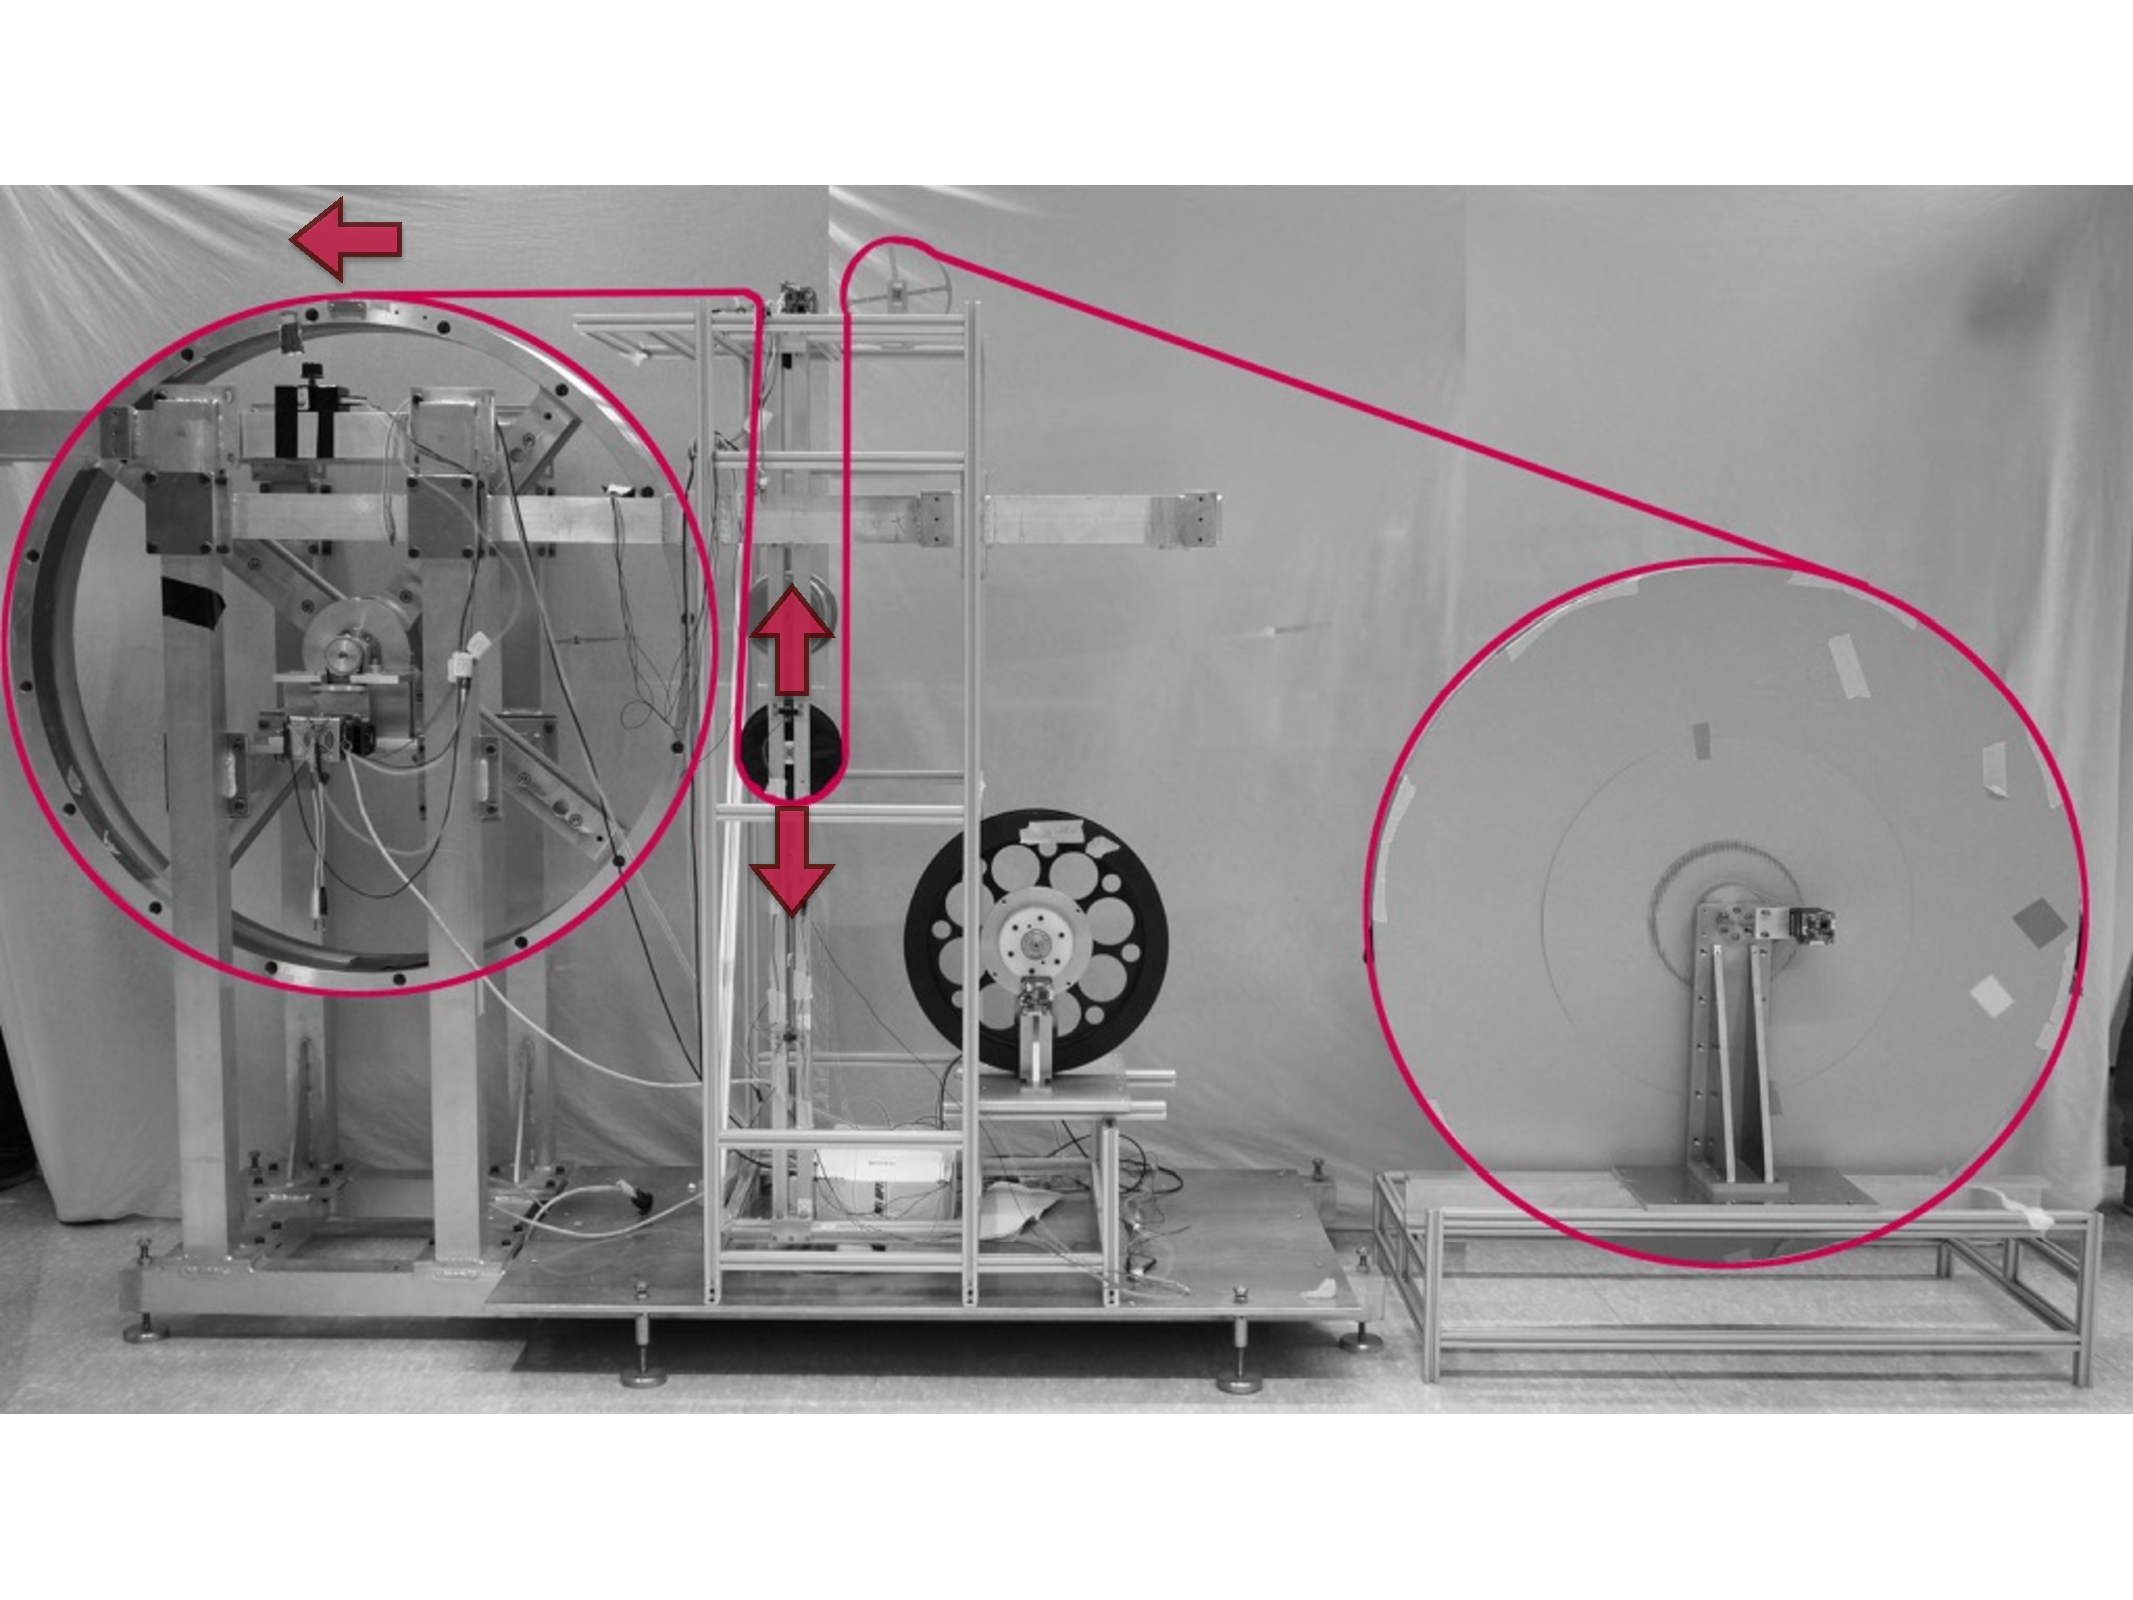
\includegraphics[width=0.75\linewidth]{figs/windingmachine}
%         \vspace*{-0.5cm}
       \end{center}
		\caption[Prototype of a winding machine to produce scintillating fibre mats.]{Prototype of a winding machine to produce scintillating fibre mats. The fibre is provided by a feeding spool (right) and moves over a loose spool to the winding wheel. The loose spool defines the tension of the fibre and regulates the speed of the feeding spool. A small spool is moving along the width of the winding wheel, for defining the correct position of the fibre.}
      	\label{fig:SciFi:WindingMachine}
   \end{figure}
   
This wheel has a milled screw to guide the fibres of the first layer and guarantee the correct pitch. At the end of the layer, the fibre is cut for starting the next layer. The layers are shifted by half the horizontal pitch with respect to each other, so that the fibres of the next layer are guided by the fibres of the respective layer before. The fibre is provided by a spool of \SI{12.5}{\kilo\metre} of scintillating fibre and is pre-guided by means of a small spool which moves along the width of the winding wheel to define the position of the fibre precisely. A loose spool in between defines the tension of the fibre and regulates the speed of the feeding spool.
$\text{TiO}_2$ loaded glue (two component epoxy) is placed between the layers. After curing the mat is cut perpendicular to the fibres and taken off the wheel to be flattenend.
For more detailed informations about the fibre mat production see also \cite{FibreMatProduction}.



\section{Quality Requirements}
\label{sec:QualityRequirements}

To ensure a spatial resolution better than \SI{100}{\micro\metre}, the fibres have to be accurately positioned. Due to many different influences problems occur during the winding process. The exclusive error is the wrong positioning of a fibre. This will manipulate the continuing fibre mat production, so that other fibres can't fit in their decided position. In the most situations the error is limited to a small region, but a small error can get worse in higher layers.
Plots shown here are the result of a winding simulation. For more Informations see \cite{WindingSimulation}.

One important point is the fluctuating diameter of the scintillating fibre. The trend of the diameter shows thick regions up to \SI{500}{\micro\metre}. These thick regions, called bumps, cause a wrong positioning of the neighbouring fibres. An example of such a error is showed in Fig. \ref{blob}.
\begin{figure}[tb]
\begin{center}
\pgfdeclareplotmark{cross} {
\pgfpathmoveto{\pgfpoint{-0.3\pgfplotmarksize}{\pgfplotmarksize}}
\pgfpathlineto{\pgfpoint{+0.3\pgfplotmarksize}{\pgfplotmarksize}}
\pgfpathlineto{\pgfpoint{+0.3\pgfplotmarksize}{0.3\pgfplotmarksize}}
\pgfpathlineto{\pgfpoint{+1\pgfplotmarksize}{0.3\pgfplotmarksize}}
\pgfpathlineto{\pgfpoint{+1\pgfplotmarksize}{-0.3\pgfplotmarksize}}
\pgfpathlineto{\pgfpoint{+0.3\pgfplotmarksize}{-0.3\pgfplotmarksize}}
\pgfpathlineto{\pgfpoint{+0.3\pgfplotmarksize}{-1.\pgfplotmarksize}}
\pgfpathlineto{\pgfpoint{-0.3\pgfplotmarksize}{-1.\pgfplotmarksize}}
\pgfpathlineto{\pgfpoint{-0.3\pgfplotmarksize}{-0.3\pgfplotmarksize}}
\pgfpathlineto{\pgfpoint{-1.\pgfplotmarksize}{-0.3\pgfplotmarksize}}
\pgfpathlineto{\pgfpoint{-1.\pgfplotmarksize}{0.3\pgfplotmarksize}}
\pgfpathlineto{\pgfpoint{-0.3\pgfplotmarksize}{0.3\pgfplotmarksize}}
\pgfpathclose
\pgfusepathqstroke
}
\pgfdeclareplotmark{cross*} {
\pgfpathmoveto{\pgfpoint{-0.3\pgfplotmarksize}{\pgfplotmarksize}}
\pgfpathlineto{\pgfpoint{+0.3\pgfplotmarksize}{\pgfplotmarksize}}
\pgfpathlineto{\pgfpoint{+0.3\pgfplotmarksize}{0.3\pgfplotmarksize}}
\pgfpathlineto{\pgfpoint{+1\pgfplotmarksize}{0.3\pgfplotmarksize}}
\pgfpathlineto{\pgfpoint{+1\pgfplotmarksize}{-0.3\pgfplotmarksize}}
\pgfpathlineto{\pgfpoint{+0.3\pgfplotmarksize}{-0.3\pgfplotmarksize}}
\pgfpathlineto{\pgfpoint{+0.3\pgfplotmarksize}{-1.\pgfplotmarksize}}
\pgfpathlineto{\pgfpoint{-0.3\pgfplotmarksize}{-1.\pgfplotmarksize}}
\pgfpathlineto{\pgfpoint{-0.3\pgfplotmarksize}{-0.3\pgfplotmarksize}}
\pgfpathlineto{\pgfpoint{-1.\pgfplotmarksize}{-0.3\pgfplotmarksize}}
\pgfpathlineto{\pgfpoint{-1.\pgfplotmarksize}{0.3\pgfplotmarksize}}
\pgfpathlineto{\pgfpoint{-0.3\pgfplotmarksize}{0.3\pgfplotmarksize}}
\pgfpathclose
\pgfusepathqfillstroke
}
\pgfdeclareplotmark{newstar} {
\pgfpathmoveto{\pgfqpoint{0pt}{\pgfplotmarksize}}
\pgfpathlineto{\pgfqpointpolar{44}{0.5\pgfplotmarksize}}
\pgfpathlineto{\pgfqpointpolar{18}{\pgfplotmarksize}}
\pgfpathlineto{\pgfqpointpolar{-20}{0.5\pgfplotmarksize}}
\pgfpathlineto{\pgfqpointpolar{-54}{\pgfplotmarksize}}
\pgfpathlineto{\pgfqpointpolar{-90}{0.5\pgfplotmarksize}}
\pgfpathlineto{\pgfqpointpolar{234}{\pgfplotmarksize}}
\pgfpathlineto{\pgfqpointpolar{198}{0.5\pgfplotmarksize}}
\pgfpathlineto{\pgfqpointpolar{162}{\pgfplotmarksize}}
\pgfpathlineto{\pgfqpointpolar{134}{0.5\pgfplotmarksize}}
\pgfpathclose
\pgfusepathqstroke
}
\pgfdeclareplotmark{newstar*} {
\pgfpathmoveto{\pgfqpoint{0pt}{\pgfplotmarksize}}
\pgfpathlineto{\pgfqpointpolar{44}{0.5\pgfplotmarksize}}
\pgfpathlineto{\pgfqpointpolar{18}{\pgfplotmarksize}}
\pgfpathlineto{\pgfqpointpolar{-20}{0.5\pgfplotmarksize}}
\pgfpathlineto{\pgfqpointpolar{-54}{\pgfplotmarksize}}
\pgfpathlineto{\pgfqpointpolar{-90}{0.5\pgfplotmarksize}}
\pgfpathlineto{\pgfqpointpolar{234}{\pgfplotmarksize}}
\pgfpathlineto{\pgfqpointpolar{198}{0.5\pgfplotmarksize}}
\pgfpathlineto{\pgfqpointpolar{162}{\pgfplotmarksize}}
\pgfpathlineto{\pgfqpointpolar{134}{0.5\pgfplotmarksize}}
\pgfpathclose
\pgfusepathqfillstroke
}
\begin{tikzpicture}[scale=0.7]
\definecolor{c}{rgb}{1,1,1};
\draw [color=c, fill=c] (0,0) rectangle (20,7.94518);
\draw [color=c, fill=c] (2,0.794518) rectangle (18,7.15066);
\definecolor{c}{rgb}{0,0,0};
\draw [c] (2,0.794518) -- (2,7.15066) -- (18,7.15066) -- (18,0.794518) -- (2,0.794518);
\draw [c] (2,0.794518) -- (18,0.794518);
\draw [anchor= east] (18,-0.049588) node[scale=1, rotate=0]{$x$ / \si{\milli\metre}};
\draw [c] (3.14286,0.985202) -- (3.14286,0.794518);
\draw [c] (3.6,0.88986) -- (3.6,0.794518);
\draw [c] (4.05714,0.88986) -- (4.05714,0.794518);
\draw [c] (4.51429,0.88986) -- (4.51429,0.794518);
\draw [c] (4.97143,0.88986) -- (4.97143,0.794518);
\draw [c] (5.42857,0.985202) -- (5.42857,0.794518);
\draw [c] (5.88571,0.88986) -- (5.88571,0.794518);
\draw [c] (6.34286,0.88986) -- (6.34286,0.794518);
\draw [c] (6.8,0.88986) -- (6.8,0.794518);
\draw [c] (7.25714,0.88986) -- (7.25714,0.794518);
\draw [c] (7.71429,0.985202) -- (7.71429,0.794518);
\draw [c] (8.17143,0.88986) -- (8.17143,0.794518);
\draw [c] (8.62857,0.88986) -- (8.62857,0.794518);
\draw [c] (9.08571,0.88986) -- (9.08571,0.794518);
\draw [c] (9.54286,0.88986) -- (9.54286,0.794518);
\draw [c] (10,0.985202) -- (10,0.794518);
\draw [c] (10.4571,0.88986) -- (10.4571,0.794518);
\draw [c] (10.9143,0.88986) -- (10.9143,0.794518);
\draw [c] (11.3714,0.88986) -- (11.3714,0.794518);
\draw [c] (11.8286,0.88986) -- (11.8286,0.794518);
\draw [c] (12.2857,0.985202) -- (12.2857,0.794518);
\draw [c] (12.7429,0.88986) -- (12.7429,0.794518);
\draw [c] (13.2,0.88986) -- (13.2,0.794518);
\draw [c] (13.6571,0.88986) -- (13.6571,0.794518);
\draw [c] (14.1143,0.88986) -- (14.1143,0.794518);
\draw [c] (14.5714,0.985202) -- (14.5714,0.794518);
\draw [c] (15.0286,0.88986) -- (15.0286,0.794518);
\draw [c] (15.4857,0.88986) -- (15.4857,0.794518);
\draw [c] (15.9429,0.88986) -- (15.9429,0.794518);
\draw [c] (16.4,0.88986) -- (16.4,0.794518);
\draw [c] (16.8571,0.985202) -- (16.8571,0.794518);
\draw [c] (3.14286,0.985202) -- (3.14286,0.794518);
\draw [c] (2.68571,0.88986) -- (2.68571,0.794518);
\draw [c] (2.22857,0.88986) -- (2.22857,0.794518);
\draw [c] (16.8571,0.985202) -- (16.8571,0.794518);
\draw [c] (17.3143,0.88986) -- (17.3143,0.794518);
\draw [c] (17.7714,0.88986) -- (17.7714,0.794518);
\draw [anchor=base] (3.14286,0.232327) node[scale=0.8, rotate=0]{92};
\draw [anchor=base] (5.42857,0.232327) node[scale=0.8, rotate=0]{92.5};
\draw [anchor=base] (7.71429,0.232327) node[scale=0.8, rotate=0]{93};
\draw [anchor=base] (10,0.232327) node[scale=0.8, rotate=0]{93.5};
\draw [anchor=base] (12.2857,0.232327) node[scale=0.8, rotate=0]{94};
\draw [anchor=base] (14.5714,0.232327) node[scale=0.8, rotate=0]{94.5};
\draw [anchor=base] (16.8571,0.232327) node[scale=0.8, rotate=0]{95};
\draw [c] (2,0.794518) -- (2,7.15066);
\draw [anchor= east] (0.68,7.15066) node[scale=1, rotate=90]{$y$ / \si{\milli\metre}};
\draw [c] (2.48,0.794518) -- (2,0.794518);
\draw [c] (2.24,1.02152) -- (2,1.02152);
\draw [c] (2.24,1.24853) -- (2,1.24853);
\draw [c] (2.24,1.47553) -- (2,1.47553);
\draw [c] (2.48,1.70254) -- (2,1.70254);
\draw [c] (2.24,1.92954) -- (2,1.92954);
\draw [c] (2.24,2.15655) -- (2,2.15655);
\draw [c] (2.24,2.38355) -- (2,2.38355);
\draw [c] (2.48,2.61056) -- (2,2.61056);
\draw [c] (2.24,2.83756) -- (2,2.83756);
\draw [c] (2.24,3.06457) -- (2,3.06457);
\draw [c] (2.24,3.29157) -- (2,3.29157);
\draw [c] (2.48,3.51858) -- (2,3.51858);
\draw [c] (2.24,3.74558) -- (2,3.74558);
\draw [c] (2.24,3.97259) -- (2,3.97259);
\draw [c] (2.24,4.19959) -- (2,4.19959);
\draw [c] (2.48,4.4266) -- (2,4.4266);
\draw [c] (2.24,4.6536) -- (2,4.6536);
\draw [c] (2.24,4.88061) -- (2,4.88061);
\draw [c] (2.24,5.10761) -- (2,5.10761);
\draw [c] (2.48,5.33462) -- (2,5.33462);
\draw [c] (2.24,5.56162) -- (2,5.56162);
\draw [c] (2.24,5.78863) -- (2,5.78863);
\draw [c] (2.24,6.01563) -- (2,6.01563);
\draw [c] (2.48,6.24264) -- (2,6.24264);
\draw [c] (2.24,6.46965) -- (2,6.46965);
\draw [c] (2.24,6.69665) -- (2,6.69665);
\draw [c] (2.24,6.92366) -- (2,6.92366);
\draw [c] (2.48,7.15066) -- (2,7.15066);
\draw [c] (2.48,7.15066) -- (2,7.15066);
\draw [anchor= east] (1.9,0.794518) node[scale=0.8, rotate=0]{0};
\draw [anchor= east] (1.9,1.70254) node[scale=0.8, rotate=0]{0.2};
\draw [anchor= east] (1.9,2.61056) node[scale=0.8, rotate=0]{0.4};
\draw [anchor= east] (1.9,3.51858) node[scale=0.8, rotate=0]{0.6};
\draw [anchor= east] (1.9,4.4266) node[scale=0.8, rotate=0]{0.8};
\draw [anchor= east] (1.9,5.33462) node[scale=0.8, rotate=0]{1};
\draw [anchor= east] (1.9,6.24264) node[scale=0.8, rotate=0]{1.2};
\draw [anchor= east] (1.9,7.15066) node[scale=0.8, rotate=0]{1.4};
\definecolor{c}{rgb}{1,1,1};
\draw [c, fill=c] (4.36616,2.06221) -- (4.34903,2.20229) -- (4.29865,2.33423) -- (4.21794,2.45036) -- (4.11159,2.54393) -- (3.98578,2.60951) -- (3.84782,2.64328) -- (3.70573,2.64328) -- (3.56778,2.60951) -- (3.44197,2.54393) -- (3.33562,2.45036) --
 (3.2549,2.33423) -- (3.20452,2.20229) -- (3.18739,2.06221) -- (3.20452,1.92212) -- (3.2549,1.79018) -- (3.33562,1.67405) -- (3.44197,1.58048) -- (3.56778,1.5149) -- (3.70573,1.48113) -- (3.84782,1.48113) -- (3.98578,1.5149) -- (4.11159,1.58048) --
 (4.21794,1.67405) -- (4.29865,1.79018) -- (4.34903,1.92212);
\definecolor{c}{rgb}{0,0,1};
\draw [c] (4.36616,2.06221) -- (4.34903,2.20229) -- (4.29865,2.33423) -- (4.21794,2.45036) -- (4.11159,2.54393) -- (3.98578,2.60951) -- (3.84782,2.64328) -- (3.70573,2.64328) -- (3.56778,2.60951) -- (3.44197,2.54393) -- (3.33562,2.45036) --
 (3.2549,2.33423) -- (3.20452,2.20229) -- (3.18739,2.06221) -- (3.20452,1.92212) -- (3.2549,1.79018) -- (3.33562,1.67405) -- (3.44197,1.58048) -- (3.56778,1.5149) -- (3.70573,1.48113) -- (3.84782,1.48113) -- (3.98578,1.5149) -- (4.11159,1.58048) --
 (4.21794,1.67405) -- (4.29865,1.79018) -- (4.34903,1.92212) -- (4.36616,2.06221);
\definecolor{c}{rgb}{1,1,1};
\draw [c, fill=c] (5.63562,2.08867) -- (5.61941,2.22649) -- (5.57162,2.35687) -- (5.49485,2.47279) -- (5.39323,2.56801) -- (5.27224,2.63738) -- (5.1384,2.67718) -- (4.99893,2.68524) -- (4.86135,2.66115) -- (4.73307,2.60619) -- (4.62101,2.52334) --
 (4.5312,2.41705) -- (4.4685,2.29306) -- (4.43628,2.15805) -- (4.43628,2.0193) -- (4.4685,1.88429) -- (4.5312,1.7603) -- (4.62101,1.65401) -- (4.73307,1.57115) -- (4.86135,1.5162) -- (4.99893,1.4921) -- (5.1384,1.50017) -- (5.27224,1.53997) --
 (5.39323,1.60934) -- (5.49485,1.70456) -- (5.57162,1.82048) -- (5.61941,1.95086);
\definecolor{c}{rgb}{0,0,1};
\draw [c] (5.63562,2.08867) -- (5.61941,2.22649) -- (5.57162,2.35687) -- (5.49485,2.47279) -- (5.39323,2.56801) -- (5.27224,2.63738) -- (5.1384,2.67718) -- (4.99893,2.68524) -- (4.86135,2.66115) -- (4.73307,2.60619) -- (4.62101,2.52334) --
 (4.5312,2.41705) -- (4.4685,2.29306) -- (4.43628,2.15805) -- (4.43628,2.0193) -- (4.4685,1.88429) -- (4.5312,1.7603) -- (4.62101,1.65401) -- (4.73307,1.57115) -- (4.86135,1.5162) -- (4.99893,1.4921) -- (5.1384,1.50017) -- (5.27224,1.53997) --
 (5.39323,1.60934) -- (5.49485,1.70456) -- (5.57162,1.82048) -- (5.61941,1.95086) -- (5.63562,2.08867);
\definecolor{c}{rgb}{1,1,1};
\draw [c, fill=c] (6.88743,2.07723) -- (6.87011,2.21898) -- (6.81912,2.35248) -- (6.73745,2.46999) -- (6.62984,2.56467) -- (6.50254,2.63103) -- (6.36295,2.6652) -- (6.21918,2.6652) -- (6.07959,2.63103) -- (5.95229,2.56467) -- (5.84467,2.46999) --
 (5.763,2.35248) -- (5.71202,2.21898) -- (5.69469,2.07723) -- (5.71202,1.93549) -- (5.763,1.80198) -- (5.84467,1.68448) -- (5.95229,1.58979) -- (6.07959,1.52344) -- (6.21918,1.48927) -- (6.36295,1.48927) -- (6.50254,1.52344) -- (6.62984,1.58979) --
 (6.73745,1.68448) -- (6.81912,1.80198) -- (6.87011,1.93549);
\definecolor{c}{rgb}{0,0,1};
\draw [c] (6.88743,2.07723) -- (6.87011,2.21898) -- (6.81912,2.35248) -- (6.73745,2.46999) -- (6.62984,2.56467) -- (6.50254,2.63103) -- (6.36295,2.6652) -- (6.21918,2.6652) -- (6.07959,2.63103) -- (5.95229,2.56467) -- (5.84467,2.46999) --
 (5.763,2.35248) -- (5.71202,2.21898) -- (5.69469,2.07723) -- (5.71202,1.93549) -- (5.763,1.80198) -- (5.84467,1.68448) -- (5.95229,1.58979) -- (6.07959,1.52344) -- (6.21918,1.48927) -- (6.36295,1.48927) -- (6.50254,1.52344) -- (6.62984,1.58979) --
 (6.73745,1.68448) -- (6.81912,1.80198) -- (6.87011,1.93549) -- (6.88743,2.07723);
\definecolor{c}{rgb}{1,1,1};
\draw [c, fill=c] (8.28513,2.29761) -- (8.27083,2.43732) -- (8.2285,2.57132) -- (8.15987,2.6941) -- (8.06777,2.80066) -- (7.95595,2.88662) -- (7.829,2.94846) -- (7.69211,2.98366) -- (7.55089,2.99078) -- (7.41112,2.96951) -- (7.27852,2.92074) --
 (7.15852,2.84645) -- (7.05603,2.7497) -- (6.97525,2.63444) -- (6.91949,2.50538) -- (6.89102,2.36783) -- (6.89102,2.22739) -- (6.91949,2.08983) -- (6.97525,1.96078) -- (7.05603,1.84552) -- (7.15852,1.74877) -- (7.27852,1.67448) -- (7.41112,1.62571)
 -- (7.55089,1.60444) -- (7.69211,1.61156) -- (7.829,1.64676) -- (7.95595,1.7086) -- (8.06777,1.79456) -- (8.15987,1.90112) -- (8.2285,2.0239) -- (8.27083,2.1579);
\definecolor{c}{rgb}{0,0,1};
\draw [c] (8.28513,2.29761) -- (8.27083,2.43732) -- (8.2285,2.57132) -- (8.15987,2.6941) -- (8.06777,2.80066) -- (7.95595,2.88662) -- (7.829,2.94846) -- (7.69211,2.98366) -- (7.55089,2.99078) -- (7.41112,2.96951) -- (7.27852,2.92074) --
 (7.15852,2.84645) -- (7.05603,2.7497) -- (6.97525,2.63444) -- (6.91949,2.50538) -- (6.89102,2.36783) -- (6.89102,2.22739) -- (6.91949,2.08983) -- (6.97525,1.96078) -- (7.05603,1.84552) -- (7.15852,1.74877) -- (7.27852,1.67448) -- (7.41112,1.62571)
 -- (7.55089,1.60444) -- (7.69211,1.61156) -- (7.829,1.64676) -- (7.95595,1.7086) -- (8.06777,1.79456) -- (8.15987,1.90112) -- (8.2285,2.0239) -- (8.27083,2.1579) -- (8.28513,2.29761);
\definecolor{c}{rgb}{1,1,1};
\draw [c, fill=c] (9.48912,2.08931) -- (9.4729,2.22719) -- (9.42509,2.35763) -- (9.34828,2.47361) -- (9.24662,2.56887) -- (9.12557,2.63828) -- (8.99167,2.67809) -- (8.85213,2.68616) -- (8.71448,2.66206) -- (8.58614,2.60708) -- (8.47402,2.52418) --
 (8.38418,2.41784) -- (8.32145,2.29379) -- (8.28921,2.15872) -- (8.28921,2.0199) -- (8.32145,1.88483) -- (8.38418,1.76078) -- (8.47402,1.65444) -- (8.58614,1.57154) -- (8.71448,1.51656) -- (8.85213,1.49246) -- (8.99167,1.50053) -- (9.12557,1.54034)
 -- (9.24662,1.60975) -- (9.34828,1.70501) -- (9.42509,1.82099) -- (9.4729,1.95143);
\definecolor{c}{rgb}{0,0,1};
\draw [c] (9.48912,2.08931) -- (9.4729,2.22719) -- (9.42509,2.35763) -- (9.34828,2.47361) -- (9.24662,2.56887) -- (9.12557,2.63828) -- (8.99167,2.67809) -- (8.85213,2.68616) -- (8.71448,2.66206) -- (8.58614,2.60708) -- (8.47402,2.52418) --
 (8.38418,2.41784) -- (8.32145,2.29379) -- (8.28921,2.15872) -- (8.28921,2.0199) -- (8.32145,1.88483) -- (8.38418,1.76078) -- (8.47402,1.65444) -- (8.58614,1.57154) -- (8.71448,1.51656) -- (8.85213,1.49246) -- (8.99167,1.50053) -- (9.12557,1.54034)
 -- (9.24662,1.60975) -- (9.34828,1.70501) -- (9.42509,1.82099) -- (9.4729,1.95143) -- (9.48912,2.08931);
\definecolor{c}{rgb}{1,1,1};
\draw [c, fill=c] (10.7315,2.05748) -- (10.7144,2.19704) -- (10.6642,2.32849) -- (10.5838,2.44419) -- (10.4778,2.53742) -- (10.3525,2.60275) -- (10.2151,2.6364) -- (10.0735,2.6364) -- (9.93605,2.60275) -- (9.81071,2.53742) -- (9.70476,2.44419) --
 (9.62434,2.32849) -- (9.57415,2.19704) -- (9.55708,2.05748) -- (9.57415,1.91792) -- (9.62434,1.78647) -- (9.70476,1.67077) -- (9.81071,1.57755) -- (9.93605,1.51221) -- (10.0735,1.47857) -- (10.2151,1.47857) -- (10.3525,1.51221) -- (10.4778,1.57755)
 -- (10.5838,1.67077) -- (10.6642,1.78647) -- (10.7144,1.91792);
\definecolor{c}{rgb}{0,0,1};
\draw [c] (10.7315,2.05748) -- (10.7144,2.19704) -- (10.6642,2.32849) -- (10.5838,2.44419) -- (10.4778,2.53742) -- (10.3525,2.60275) -- (10.2151,2.6364) -- (10.0735,2.6364) -- (9.93605,2.60275) -- (9.81071,2.53742) -- (9.70476,2.44419) --
 (9.62434,2.32849) -- (9.57415,2.19704) -- (9.55708,2.05748) -- (9.57415,1.91792) -- (9.62434,1.78647) -- (9.70476,1.67077) -- (9.81071,1.57755) -- (9.93605,1.51221) -- (10.0735,1.47857) -- (10.2151,1.47857) -- (10.3525,1.51221) -- (10.4778,1.57755)
 -- (10.5838,1.67077) -- (10.6642,1.78647) -- (10.7144,1.91792) -- (10.7315,2.05748);
\definecolor{c}{rgb}{1,1,1};
\draw [c, fill=c] (11.9916,2.06398) -- (11.9745,2.20426) -- (11.924,2.33638) -- (11.8432,2.45268) -- (11.7367,2.54639) -- (11.6107,2.61206) -- (11.4726,2.64587) -- (11.3303,2.64587) -- (11.1921,2.61206) -- (11.0661,2.54639) -- (10.9596,2.45268) --
 (10.8788,2.33638) -- (10.8284,2.20426) -- (10.8112,2.06398) -- (10.8284,1.9237) -- (10.8788,1.79157) -- (10.9596,1.67527) -- (11.0661,1.58156) -- (11.1921,1.51589) -- (11.3303,1.48208) -- (11.4726,1.48208) -- (11.6107,1.51589) -- (11.7367,1.58156)
 -- (11.8432,1.67527) -- (11.924,1.79157) -- (11.9745,1.9237);
\definecolor{c}{rgb}{0,0,1};
\draw [c] (11.9916,2.06398) -- (11.9745,2.20426) -- (11.924,2.33638) -- (11.8432,2.45268) -- (11.7367,2.54639) -- (11.6107,2.61206) -- (11.4726,2.64587) -- (11.3303,2.64587) -- (11.1921,2.61206) -- (11.0661,2.54639) -- (10.9596,2.45268) --
 (10.8788,2.33638) -- (10.8284,2.20426) -- (10.8112,2.06398) -- (10.8284,1.9237) -- (10.8788,1.79157) -- (10.9596,1.67527) -- (11.0661,1.58156) -- (11.1921,1.51589) -- (11.3303,1.48208) -- (11.4726,1.48208) -- (11.6107,1.51589) -- (11.7367,1.58156)
 -- (11.8432,1.67527) -- (11.924,1.79157) -- (11.9745,1.9237) -- (11.9916,2.06398);
\definecolor{c}{rgb}{1,1,1};
\draw [c, fill=c] (13.2701,2.10974) -- (13.2536,2.2498) -- (13.205,2.3823) -- (13.127,2.50011) -- (13.0237,2.59688) -- (12.9008,2.66738) -- (12.7647,2.70782) -- (12.623,2.71602) -- (12.4832,2.69154) -- (12.3528,2.63569) -- (12.2389,2.55148) --
 (12.1477,2.44346) -- (12.0839,2.31745) -- (12.0512,2.18024) -- (12.0512,2.03924) -- (12.0839,1.90203) -- (12.1477,1.77602) -- (12.2389,1.668) -- (12.3528,1.58379) -- (12.4832,1.52794) -- (12.623,1.50346) -- (12.7647,1.51166) -- (12.9008,1.5521) --
 (13.0237,1.6226) -- (13.127,1.71937) -- (13.205,1.83718) -- (13.2536,1.96968);
\definecolor{c}{rgb}{0,0,1};
\draw [c] (13.2701,2.10974) -- (13.2536,2.2498) -- (13.205,2.3823) -- (13.127,2.50011) -- (13.0237,2.59688) -- (12.9008,2.66738) -- (12.7647,2.70782) -- (12.623,2.71602) -- (12.4832,2.69154) -- (12.3528,2.63569) -- (12.2389,2.55148) --
 (12.1477,2.44346) -- (12.0839,2.31745) -- (12.0512,2.18024) -- (12.0512,2.03924) -- (12.0839,1.90203) -- (12.1477,1.77602) -- (12.2389,1.668) -- (12.3528,1.58379) -- (12.4832,1.52794) -- (12.623,1.50346) -- (12.7647,1.51166) -- (12.9008,1.5521) --
 (13.0237,1.6226) -- (13.127,1.71937) -- (13.205,1.83718) -- (13.2536,1.96968) -- (13.2701,2.10974);
\definecolor{c}{rgb}{1,1,1};
\draw [c, fill=c] (14.5236,2.10198) -- (14.5072,2.2412) -- (14.4589,2.37293) -- (14.3814,2.49004) -- (14.2787,2.58623) -- (14.1565,2.65632) -- (14.0213,2.69652) -- (13.8804,2.70467) -- (13.7414,2.68033) -- (13.6118,2.62481) -- (13.4985,2.54111) --
 (13.4078,2.43373) -- (13.3445,2.30846) -- (13.3119,2.17206) -- (13.3119,2.03189) -- (13.3445,1.89549) -- (13.4078,1.77023) -- (13.4985,1.66285) -- (13.6118,1.57914) -- (13.7414,1.52362) -- (13.8804,1.49928) -- (14.0213,1.50743) -- (14.1565,1.54763)
 -- (14.2787,1.61772) -- (14.3814,1.71391) -- (14.4589,1.83103) -- (14.5072,1.96275);
\definecolor{c}{rgb}{0,0,1};
\draw [c] (14.5236,2.10198) -- (14.5072,2.2412) -- (14.4589,2.37293) -- (14.3814,2.49004) -- (14.2787,2.58623) -- (14.1565,2.65632) -- (14.0213,2.69652) -- (13.8804,2.70467) -- (13.7414,2.68033) -- (13.6118,2.62481) -- (13.4985,2.54111) --
 (13.4078,2.43373) -- (13.3445,2.30846) -- (13.3119,2.17206) -- (13.3119,2.03189) -- (13.3445,1.89549) -- (13.4078,1.77023) -- (13.4985,1.66285) -- (13.6118,1.57914) -- (13.7414,1.52362) -- (13.8804,1.49928) -- (14.0213,1.50743) -- (14.1565,1.54763)
 -- (14.2787,1.61772) -- (14.3814,1.71391) -- (14.4589,1.83103) -- (14.5072,1.96275) -- (14.5236,2.10198);
\definecolor{c}{rgb}{1,1,1};
\draw [c, fill=c] (15.7749,2.0894) -- (15.7587,2.22729) -- (15.7109,2.35775) -- (15.634,2.47374) -- (15.5324,2.569) -- (15.4113,2.63842) -- (15.2774,2.67824) -- (15.1378,2.68631) -- (15.0002,2.6622) -- (14.8718,2.60721) -- (14.7597,2.52431) --
 (14.6698,2.41796) -- (14.6071,2.2939) -- (14.5749,2.15881) -- (14.5749,2.01999) -- (14.6071,1.8849) -- (14.6698,1.76084) -- (14.7597,1.65449) -- (14.8718,1.57159) -- (15.0002,1.5166) -- (15.1378,1.49249) -- (15.2774,1.50057) -- (15.4113,1.54038) --
 (15.5324,1.6098) -- (15.634,1.70507) -- (15.7109,1.82105) -- (15.7587,1.95151);
\definecolor{c}{rgb}{0,0,1};
\draw [c] (15.7749,2.0894) -- (15.7587,2.22729) -- (15.7109,2.35775) -- (15.634,2.47374) -- (15.5324,2.569) -- (15.4113,2.63842) -- (15.2774,2.67824) -- (15.1378,2.68631) -- (15.0002,2.6622) -- (14.8718,2.60721) -- (14.7597,2.52431) --
 (14.6698,2.41796) -- (14.6071,2.2939) -- (14.5749,2.15881) -- (14.5749,2.01999) -- (14.6071,1.8849) -- (14.6698,1.76084) -- (14.7597,1.65449) -- (14.8718,1.57159) -- (15.0002,1.5166) -- (15.1378,1.49249) -- (15.2774,1.50057) -- (15.4113,1.54038) --
 (15.5324,1.6098) -- (15.634,1.70507) -- (15.7109,1.82105) -- (15.7587,1.95151) -- (15.7749,2.0894);
\definecolor{c}{rgb}{1,1,1};
\draw [c, fill=c] (17.0217,2.0672) -- (17.0045,2.20784) -- (16.9539,2.3403) -- (16.8729,2.4569) -- (16.7661,2.55084) -- (16.6398,2.61668) -- (16.5013,2.65058) -- (16.3587,2.65058) -- (16.2202,2.61668) -- (16.0939,2.55084) -- (15.9871,2.4569) --
 (15.906,2.3403) -- (15.8555,2.20784) -- (15.8383,2.0672) -- (15.8555,1.92656) -- (15.906,1.7941) -- (15.9871,1.6775) -- (16.0939,1.58356) -- (16.2202,1.51772) -- (16.3587,1.48382) -- (16.5013,1.48382) -- (16.6398,1.51772) -- (16.7661,1.58356) --
 (16.8729,1.6775) -- (16.9539,1.7941) -- (17.0045,1.92656);
\definecolor{c}{rgb}{0,0,1};
\draw [c] (17.0217,2.0672) -- (17.0045,2.20784) -- (16.9539,2.3403) -- (16.8729,2.4569) -- (16.7661,2.55084) -- (16.6398,2.61668) -- (16.5013,2.65058) -- (16.3587,2.65058) -- (16.2202,2.61668) -- (16.0939,2.55084) -- (15.9871,2.4569) --
 (15.906,2.3403) -- (15.8555,2.20784) -- (15.8383,2.0672) -- (15.8555,1.92656) -- (15.906,1.7941) -- (15.9871,1.6775) -- (16.0939,1.58356) -- (16.2202,1.51772) -- (16.3587,1.48382) -- (16.5013,1.48382) -- (16.6398,1.51772) -- (16.7661,1.58356) --
 (16.8729,1.6775) -- (16.9539,1.7941) -- (17.0045,1.92656) -- (17.0217,2.0672);
\definecolor{c}{rgb}{1,1,1};
\draw [c, fill=c] (3.79246,3.10802) -- (3.77507,3.25024) -- (3.72392,3.3842) -- (3.64197,3.50211) -- (3.53399,3.59712) -- (3.40625,3.6637) -- (3.26619,3.69798) -- (3.12193,3.69798) -- (2.98186,3.6637) -- (2.85413,3.59712) -- (2.74615,3.50211) --
 (2.6642,3.3842) -- (2.61304,3.25024) -- (2.59566,3.10802) -- (2.61304,2.96579) -- (2.6642,2.83183) -- (2.74615,2.71392) -- (2.85413,2.61892) -- (2.98186,2.55234) -- (3.12193,2.51805) -- (3.26619,2.51805) -- (3.40625,2.55234) -- (3.53399,2.61892) --
 (3.64197,2.71392) -- (3.72392,2.83183) -- (3.77507,2.96579);
\definecolor{c}{rgb}{1,0,0};
\draw [c] (3.79246,3.10802) -- (3.77507,3.25024) -- (3.72392,3.3842) -- (3.64197,3.50211) -- (3.53399,3.59712) -- (3.40625,3.6637) -- (3.26619,3.69798) -- (3.12193,3.69798) -- (2.98186,3.6637) -- (2.85413,3.59712) -- (2.74615,3.50211) --
 (2.6642,3.3842) -- (2.61304,3.25024) -- (2.59566,3.10802) -- (2.61304,2.96579) -- (2.6642,2.83183) -- (2.74615,2.71392) -- (2.85413,2.61892) -- (2.98186,2.55234) -- (3.12193,2.51805) -- (3.26619,2.51805) -- (3.40625,2.55234) -- (3.53399,2.61892) --
 (3.64197,2.71392) -- (3.72392,2.83183) -- (3.77507,2.96579) -- (3.79246,3.10802);
\definecolor{c}{rgb}{1,1,1};
\draw [c, fill=c] (4.99223,3.09217) -- (4.97484,3.2344) -- (4.92369,3.36836) -- (4.84174,3.48627) -- (4.73376,3.58127) -- (4.60602,3.64785) -- (4.46596,3.68214) -- (4.3217,3.68214) -- (4.18163,3.64785) -- (4.0539,3.58127) -- (3.94592,3.48627) --
 (3.86397,3.36836) -- (3.81282,3.2344) -- (3.79543,3.09217) -- (3.81282,2.94995) -- (3.86397,2.81599) -- (3.94592,2.69808) -- (4.0539,2.60307) -- (4.18163,2.53649) -- (4.3217,2.50221) -- (4.46596,2.50221) -- (4.60602,2.53649) -- (4.73376,2.60307) --
 (4.84174,2.69808) -- (4.92369,2.81599) -- (4.97484,2.94995);
\definecolor{c}{rgb}{1,0,0};
\draw [c] (4.99223,3.09217) -- (4.97484,3.2344) -- (4.92369,3.36836) -- (4.84174,3.48627) -- (4.73376,3.58127) -- (4.60602,3.64785) -- (4.46596,3.68214) -- (4.3217,3.68214) -- (4.18163,3.64785) -- (4.0539,3.58127) -- (3.94592,3.48627) --
 (3.86397,3.36836) -- (3.81282,3.2344) -- (3.79543,3.09217) -- (3.81282,2.94995) -- (3.86397,2.81599) -- (3.94592,2.69808) -- (4.0539,2.60307) -- (4.18163,2.53649) -- (4.3217,2.50221) -- (4.46596,2.50221) -- (4.60602,2.53649) -- (4.73376,2.60307) --
 (4.84174,2.69808) -- (4.92369,2.81599) -- (4.97484,2.94995) -- (4.99223,3.09217);
\definecolor{c}{rgb}{1,1,1};
\draw [c, fill=c] (6.27717,3.12277) -- (6.25978,3.265) -- (6.20862,3.39896) -- (6.12668,3.51687) -- (6.0187,3.61187) -- (5.89096,3.67845) -- (5.7509,3.71274) -- (5.60664,3.71274) -- (5.46657,3.67845) -- (5.33884,3.61187) -- (5.23086,3.51687) --
 (5.14891,3.39896) -- (5.09775,3.265) -- (5.08036,3.12277) -- (5.09775,2.98055) -- (5.14891,2.84659) -- (5.23086,2.72868) -- (5.33884,2.63367) -- (5.46657,2.56709) -- (5.60664,2.53281) -- (5.7509,2.53281) -- (5.89096,2.56709) -- (6.0187,2.63367) --
 (6.12668,2.72868) -- (6.20862,2.84659) -- (6.25978,2.98055);
\definecolor{c}{rgb}{1,0,0};
\draw [c] (6.27717,3.12277) -- (6.25978,3.265) -- (6.20862,3.39896) -- (6.12668,3.51687) -- (6.0187,3.61187) -- (5.89096,3.67845) -- (5.7509,3.71274) -- (5.60664,3.71274) -- (5.46657,3.67845) -- (5.33884,3.61187) -- (5.23086,3.51687) --
 (5.14891,3.39896) -- (5.09775,3.265) -- (5.08036,3.12277) -- (5.09775,2.98055) -- (5.14891,2.84659) -- (5.23086,2.72868) -- (5.33884,2.63367) -- (5.46657,2.56709) -- (5.60664,2.53281) -- (5.7509,2.53281) -- (5.89096,2.56709) -- (6.0187,2.63367) --
 (6.12668,2.72868) -- (6.20862,2.84659) -- (6.25978,2.98055) -- (6.27717,3.12277);
\definecolor{c}{rgb}{1,1,1};
\draw [c, fill=c] (7.46684,3.38487) -- (7.44945,3.5271) -- (7.39829,3.66106) -- (7.31634,3.77897) -- (7.20836,3.87397) -- (7.08063,3.94055) -- (6.94056,3.97484) -- (6.79631,3.97484) -- (6.65624,3.94055) -- (6.5285,3.87397) -- (6.42052,3.77897) --
 (6.33858,3.66106) -- (6.28742,3.5271) -- (6.27003,3.38487) -- (6.28742,3.24265) -- (6.33858,3.10869) -- (6.42052,2.99078) -- (6.5285,2.89577) -- (6.65624,2.82919) -- (6.79631,2.79491) -- (6.94056,2.79491) -- (7.08063,2.82919) -- (7.20836,2.89577) --
 (7.31634,2.99078) -- (7.39829,3.10869) -- (7.44945,3.24265);
\definecolor{c}{rgb}{1,0,0};
\draw [c] (7.46684,3.38487) -- (7.44945,3.5271) -- (7.39829,3.66106) -- (7.31634,3.77897) -- (7.20836,3.87397) -- (7.08063,3.94055) -- (6.94056,3.97484) -- (6.79631,3.97484) -- (6.65624,3.94055) -- (6.5285,3.87397) -- (6.42052,3.77897) --
 (6.33858,3.66106) -- (6.28742,3.5271) -- (6.27003,3.38487) -- (6.28742,3.24265) -- (6.33858,3.10869) -- (6.42052,2.99078) -- (6.5285,2.89577) -- (6.65624,2.82919) -- (6.79631,2.79491) -- (6.94056,2.79491) -- (7.08063,2.82919) -- (7.20836,2.89577) --
 (7.31634,2.99078) -- (7.39829,3.10869) -- (7.44945,3.24265) -- (7.46684,3.38487);
\definecolor{c}{rgb}{1,1,1};
\draw [c, fill=c] (9.10601,3.2321) -- (9.08862,3.37432) -- (9.03747,3.50828) -- (8.95552,3.62619) -- (8.84754,3.7212) -- (8.71981,3.78778) -- (8.57974,3.82207) -- (8.43548,3.82207) -- (8.29542,3.78778) -- (8.16768,3.7212) -- (8.0597,3.62619) --
 (7.97775,3.50828) -- (7.9266,3.37432) -- (7.90921,3.2321) -- (7.9266,3.08987) -- (7.97775,2.95591) -- (8.0597,2.838) -- (8.16768,2.743) -- (8.29542,2.67642) -- (8.43548,2.64213) -- (8.57974,2.64213) -- (8.71981,2.67642) -- (8.84754,2.743) --
 (8.95552,2.838) -- (9.03747,2.95591) -- (9.08862,3.08987);
\definecolor{c}{rgb}{1,0,0};
\draw [c] (9.10601,3.2321) -- (9.08862,3.37432) -- (9.03747,3.50828) -- (8.95552,3.62619) -- (8.84754,3.7212) -- (8.71981,3.78778) -- (8.57974,3.82207) -- (8.43548,3.82207) -- (8.29542,3.78778) -- (8.16768,3.7212) -- (8.0597,3.62619) --
 (7.97775,3.50828) -- (7.9266,3.37432) -- (7.90921,3.2321) -- (7.9266,3.08987) -- (7.97775,2.95591) -- (8.0597,2.838) -- (8.16768,2.743) -- (8.29542,2.67642) -- (8.43548,2.64213) -- (8.57974,2.64213) -- (8.71981,2.67642) -- (8.84754,2.743) --
 (8.95552,2.838) -- (9.03747,2.95591) -- (9.08862,3.08987) -- (9.10601,3.2321);
\definecolor{c}{rgb}{1,1,1};
\draw [c, fill=c] (10.3183,3.1822) -- (10.3009,3.32443) -- (10.2498,3.45839) -- (10.1678,3.5763) -- (10.0598,3.6713) -- (9.9321,3.73788) -- (9.79204,3.77217) -- (9.64778,3.77217) -- (9.50771,3.73788) -- (9.37998,3.6713) -- (9.272,3.5763) --
 (9.19005,3.45839) -- (9.1389,3.32443) -- (9.12151,3.1822) -- (9.1389,3.03998) -- (9.19005,2.90602) -- (9.272,2.78811) -- (9.37998,2.6931) -- (9.50771,2.62652) -- (9.64778,2.59224) -- (9.79204,2.59224) -- (9.9321,2.62652) -- (10.0598,2.6931) --
 (10.1678,2.78811) -- (10.2498,2.90602) -- (10.3009,3.03998);
\definecolor{c}{rgb}{1,0,0};
\draw [c] (10.3183,3.1822) -- (10.3009,3.32443) -- (10.2498,3.45839) -- (10.1678,3.5763) -- (10.0598,3.6713) -- (9.9321,3.73788) -- (9.79204,3.77217) -- (9.64778,3.77217) -- (9.50771,3.73788) -- (9.37998,3.6713) -- (9.272,3.5763) -- (9.19005,3.45839)
 -- (9.1389,3.32443) -- (9.12151,3.1822) -- (9.1389,3.03998) -- (9.19005,2.90602) -- (9.272,2.78811) -- (9.37998,2.6931) -- (9.50771,2.62652) -- (9.64778,2.59224) -- (9.79204,2.59224) -- (9.9321,2.62652) -- (10.0598,2.6931) -- (10.1678,2.78811) --
 (10.2498,2.90602) -- (10.3009,3.03998) -- (10.3183,3.1822);
\definecolor{c}{rgb}{1,1,1};
\draw [c, fill=c] (11.5206,3.1423) -- (11.5032,3.28452) -- (11.4521,3.41848) -- (11.3701,3.53639) -- (11.2621,3.63139) -- (11.1344,3.69798) -- (10.9943,3.73226) -- (10.8501,3.73226) -- (10.71,3.69798) -- (10.5823,3.63139) -- (10.4743,3.53639) --
 (10.3923,3.41848) -- (10.3412,3.28452) -- (10.3238,3.1423) -- (10.3412,3.00007) -- (10.3923,2.86611) -- (10.4743,2.7482) -- (10.5823,2.6532) -- (10.71,2.58661) -- (10.8501,2.55233) -- (10.9943,2.55233) -- (11.1344,2.58661) -- (11.2621,2.6532) --
 (11.3701,2.7482) -- (11.4521,2.86611) -- (11.5032,3.00007);
\definecolor{c}{rgb}{1,0,0};
\draw [c] (11.5206,3.1423) -- (11.5032,3.28452) -- (11.4521,3.41848) -- (11.3701,3.53639) -- (11.2621,3.63139) -- (11.1344,3.69798) -- (10.9943,3.73226) -- (10.8501,3.73226) -- (10.71,3.69798) -- (10.5823,3.63139) -- (10.4743,3.53639) --
 (10.3923,3.41848) -- (10.3412,3.28452) -- (10.3238,3.1423) -- (10.3412,3.00007) -- (10.3923,2.86611) -- (10.4743,2.7482) -- (10.5823,2.6532) -- (10.71,2.58661) -- (10.8501,2.55233) -- (10.9943,2.55233) -- (11.1344,2.58661) -- (11.2621,2.6532) --
 (11.3701,2.7482) -- (11.4521,2.86611) -- (11.5032,3.00007) -- (11.5206,3.1423);
\definecolor{c}{rgb}{1,1,1};
\draw [c, fill=c] (12.7334,3.19632) -- (12.716,3.33855) -- (12.6649,3.47251) -- (12.5829,3.59042) -- (12.4749,3.68542) -- (12.3472,3.752) -- (12.2071,3.78629) -- (12.0629,3.78629) -- (11.9228,3.752) -- (11.7951,3.68542) -- (11.6871,3.59042) --
 (11.6051,3.47251) -- (11.554,3.33855) -- (11.5366,3.19632) -- (11.554,3.0541) -- (11.6051,2.92014) -- (11.6871,2.80223) -- (11.7951,2.70722) -- (11.9228,2.64064) -- (12.0629,2.60636) -- (12.2071,2.60636) -- (12.3472,2.64064) -- (12.4749,2.70722) --
 (12.5829,2.80223) -- (12.6649,2.92014) -- (12.716,3.0541);
\definecolor{c}{rgb}{1,0,0};
\draw [c] (12.7334,3.19632) -- (12.716,3.33855) -- (12.6649,3.47251) -- (12.5829,3.59042) -- (12.4749,3.68542) -- (12.3472,3.752) -- (12.2071,3.78629) -- (12.0629,3.78629) -- (11.9228,3.752) -- (11.7951,3.68542) -- (11.6871,3.59042) --
 (11.6051,3.47251) -- (11.554,3.33855) -- (11.5366,3.19632) -- (11.554,3.0541) -- (11.6051,2.92014) -- (11.6871,2.80223) -- (11.7951,2.70722) -- (11.9228,2.64064) -- (12.0629,2.60636) -- (12.2071,2.60636) -- (12.3472,2.64064) -- (12.4749,2.70722) --
 (12.5829,2.80223) -- (12.6649,2.92014) -- (12.716,3.0541) -- (12.7334,3.19632);
\definecolor{c}{rgb}{1,1,1};
\draw [c, fill=c] (13.9481,3.19219) -- (13.9307,3.33442) -- (13.8795,3.46838) -- (13.7976,3.58629) -- (13.6896,3.68129) -- (13.5619,3.74787) -- (13.4218,3.78216) -- (13.2775,3.78216) -- (13.1375,3.74787) -- (13.0097,3.68129) -- (12.9018,3.58629) --
 (12.8198,3.46838) -- (12.7687,3.33442) -- (12.7513,3.19219) -- (12.7687,3.04997) -- (12.8198,2.91601) -- (12.9018,2.7981) -- (13.0097,2.70309) -- (13.1375,2.63651) -- (13.2775,2.60222) -- (13.4218,2.60222) -- (13.5619,2.63651) -- (13.6896,2.70309)
 -- (13.7976,2.7981) -- (13.8795,2.91601) -- (13.9307,3.04997);
\definecolor{c}{rgb}{1,0,0};
\draw [c] (13.9481,3.19219) -- (13.9307,3.33442) -- (13.8795,3.46838) -- (13.7976,3.58629) -- (13.6896,3.68129) -- (13.5619,3.74787) -- (13.4218,3.78216) -- (13.2775,3.78216) -- (13.1375,3.74787) -- (13.0097,3.68129) -- (12.9018,3.58629) --
 (12.8198,3.46838) -- (12.7687,3.33442) -- (12.7513,3.19219) -- (12.7687,3.04997) -- (12.8198,2.91601) -- (12.9018,2.7981) -- (13.0097,2.70309) -- (13.1375,2.63651) -- (13.2775,2.60222) -- (13.4218,2.60222) -- (13.5619,2.63651) -- (13.6896,2.70309)
 -- (13.7976,2.7981) -- (13.8795,2.91601) -- (13.9307,3.04997) -- (13.9481,3.19219);
\definecolor{c}{rgb}{1,1,1};
\draw [c, fill=c] (15.1469,3.10307) -- (15.1295,3.24529) -- (15.0783,3.37925) -- (14.9964,3.49716) -- (14.8884,3.59217) -- (14.7607,3.65875) -- (14.6206,3.69304) -- (14.4764,3.69304) -- (14.3363,3.65875) -- (14.2085,3.59217) -- (14.1006,3.49716) --
 (14.0186,3.37925) -- (13.9675,3.24529) -- (13.9501,3.10307) -- (13.9675,2.96084) -- (14.0186,2.82688) -- (14.1006,2.70897) -- (14.2085,2.61397) -- (14.3363,2.54739) -- (14.4764,2.5131) -- (14.6206,2.5131) -- (14.7607,2.54739) -- (14.8884,2.61397) --
 (14.9964,2.70897) -- (15.0783,2.82688) -- (15.1295,2.96084);
\definecolor{c}{rgb}{1,0,0};
\draw [c] (15.1469,3.10307) -- (15.1295,3.24529) -- (15.0783,3.37925) -- (14.9964,3.49716) -- (14.8884,3.59217) -- (14.7607,3.65875) -- (14.6206,3.69304) -- (14.4764,3.69304) -- (14.3363,3.65875) -- (14.2085,3.59217) -- (14.1006,3.49716) --
 (14.0186,3.37925) -- (13.9675,3.24529) -- (13.9501,3.10307) -- (13.9675,2.96084) -- (14.0186,2.82688) -- (14.1006,2.70897) -- (14.2085,2.61397) -- (14.3363,2.54739) -- (14.4764,2.5131) -- (14.6206,2.5131) -- (14.7607,2.54739) -- (14.8884,2.61397) --
 (14.9964,2.70897) -- (15.0783,2.82688) -- (15.1295,2.96084) -- (15.1469,3.10307);
\definecolor{c}{rgb}{1,1,1};
\draw [c, fill=c] (16.4242,3.12114) -- (16.4068,3.26336) -- (16.3556,3.39732) -- (16.2737,3.51523) -- (16.1657,3.61024) -- (16.038,3.67682) -- (15.8979,3.71111) -- (15.7537,3.71111) -- (15.6136,3.67682) -- (15.4859,3.61024) -- (15.3779,3.51523) --
 (15.2959,3.39732) -- (15.2448,3.26336) -- (15.2274,3.12114) -- (15.2448,2.97891) -- (15.2959,2.84495) -- (15.3779,2.72704) -- (15.4859,2.63204) -- (15.6136,2.56546) -- (15.7537,2.53117) -- (15.8979,2.53117) -- (16.038,2.56546) -- (16.1657,2.63204)
 -- (16.2737,2.72704) -- (16.3556,2.84495) -- (16.4068,2.97891);
\definecolor{c}{rgb}{1,0,0};
\draw [c] (16.4242,3.12114) -- (16.4068,3.26336) -- (16.3556,3.39732) -- (16.2737,3.51523) -- (16.1657,3.61024) -- (16.038,3.67682) -- (15.8979,3.71111) -- (15.7537,3.71111) -- (15.6136,3.67682) -- (15.4859,3.61024) -- (15.3779,3.51523) --
 (15.2959,3.39732) -- (15.2448,3.26336) -- (15.2274,3.12114) -- (15.2448,2.97891) -- (15.2959,2.84495) -- (15.3779,2.72704) -- (15.4859,2.63204) -- (15.6136,2.56546) -- (15.7537,2.53117) -- (15.8979,2.53117) -- (16.038,2.56546) -- (16.1657,2.63204)
 -- (16.2737,2.72704) -- (16.3556,2.84495) -- (16.4068,2.97891) -- (16.4242,3.12114);
\definecolor{c}{rgb}{1,1,1};
\draw [c, fill=c] (4.42624,4.15787) -- (4.40999,4.29592) -- (4.36212,4.42653) -- (4.28522,4.54265) -- (4.18343,4.63803) -- (4.06223,4.70752) -- (3.92816,4.74739) -- (3.78845,4.75547) -- (3.65063,4.73133) -- (3.52213,4.67628) -- (3.40987,4.59328) --
 (3.31992,4.48681) -- (3.25711,4.36261) -- (3.22483,4.22737) -- (3.22483,4.08838) -- (3.25711,3.95313) -- (3.31992,3.82893) -- (3.40987,3.72246) -- (3.52213,3.63946) -- (3.65063,3.58441) -- (3.78845,3.56027) -- (3.92816,3.56836) -- (4.06223,3.60822)
 -- (4.18343,3.67771) -- (4.28522,3.77309) -- (4.36212,3.88922) -- (4.40999,4.01982);
\definecolor{c}{rgb}{0,1,0};
\draw [c] (4.42624,4.15787) -- (4.40999,4.29592) -- (4.36212,4.42653) -- (4.28522,4.54265) -- (4.18343,4.63803) -- (4.06223,4.70752) -- (3.92816,4.74739) -- (3.78845,4.75547) -- (3.65063,4.73133) -- (3.52213,4.67628) -- (3.40987,4.59328) --
 (3.31992,4.48681) -- (3.25711,4.36261) -- (3.22483,4.22737) -- (3.22483,4.08838) -- (3.25711,3.95313) -- (3.31992,3.82893) -- (3.40987,3.72246) -- (3.52213,3.63946) -- (3.65063,3.58441) -- (3.78845,3.56027) -- (3.92816,3.56836) -- (4.06223,3.60822)
 -- (4.18343,3.67771) -- (4.28522,3.77309) -- (4.36212,3.88922) -- (4.40999,4.01982) -- (4.42624,4.15787);
\definecolor{c}{rgb}{1,1,1};
\draw [c, fill=c] (5.6304,4.14561) -- (5.61415,4.28366) -- (5.56628,4.41427) -- (5.48938,4.53039) -- (5.38759,4.62577) -- (5.26639,4.69526) -- (5.13232,4.73513) -- (4.99261,4.74321) -- (4.85479,4.71907) -- (4.72629,4.66402) -- (4.61403,4.58102) --
 (4.52408,4.47455) -- (4.46127,4.35035) -- (4.42899,4.21511) -- (4.42899,4.07612) -- (4.46127,3.94088) -- (4.52408,3.81667) -- (4.61403,3.7102) -- (4.72629,3.6272) -- (4.85479,3.57215) -- (4.99261,3.54802) -- (5.13232,3.5561) -- (5.26639,3.59596) --
 (5.38759,3.66545) -- (5.48938,3.76083) -- (5.56628,3.87696) -- (5.61415,4.00756);
\definecolor{c}{rgb}{0,1,0};
\draw [c] (5.6304,4.14561) -- (5.61415,4.28366) -- (5.56628,4.41427) -- (5.48938,4.53039) -- (5.38759,4.62577) -- (5.26639,4.69526) -- (5.13232,4.73513) -- (4.99261,4.74321) -- (4.85479,4.71907) -- (4.72629,4.66402) -- (4.61403,4.58102) --
 (4.52408,4.47455) -- (4.46127,4.35035) -- (4.42899,4.21511) -- (4.42899,4.07612) -- (4.46127,3.94088) -- (4.52408,3.81667) -- (4.61403,3.7102) -- (4.72629,3.6272) -- (4.85479,3.57215) -- (4.99261,3.54802) -- (5.13232,3.5561) -- (5.26639,3.59596) --
 (5.38759,3.66545) -- (5.48938,3.76083) -- (5.56628,3.87696) -- (5.61415,4.00756) -- (5.6304,4.14561);
\definecolor{c}{rgb}{1,1,1};
\draw [c, fill=c] (6.83766,4.41952) -- (6.82142,4.55757) -- (6.77355,4.68817) -- (6.69665,4.80429) -- (6.59486,4.89967) -- (6.47366,4.96917) -- (6.33959,5.00903) -- (6.19988,5.01711) -- (6.06206,4.99298) -- (5.93356,4.93793) -- (5.8213,4.85493) --
 (5.73134,4.74846) -- (5.66854,4.62425) -- (5.63626,4.48901) -- (5.63626,4.35002) -- (5.66854,4.21478) -- (5.73134,4.09058) -- (5.8213,3.9841) -- (5.93356,3.90111) -- (6.06206,3.84606) -- (6.19988,3.82192) -- (6.33959,3.83) -- (6.47366,3.86986) --
 (6.59486,3.93936) -- (6.69665,4.03474) -- (6.77355,4.15086) -- (6.82142,4.28147);
\definecolor{c}{rgb}{0,1,0};
\draw [c] (6.83766,4.41952) -- (6.82142,4.55757) -- (6.77355,4.68817) -- (6.69665,4.80429) -- (6.59486,4.89967) -- (6.47366,4.96917) -- (6.33959,5.00903) -- (6.19988,5.01711) -- (6.06206,4.99298) -- (5.93356,4.93793) -- (5.8213,4.85493) --
 (5.73134,4.74846) -- (5.66854,4.62425) -- (5.63626,4.48901) -- (5.63626,4.35002) -- (5.66854,4.21478) -- (5.73134,4.09058) -- (5.8213,3.9841) -- (5.93356,3.90111) -- (6.06206,3.84606) -- (6.19988,3.82192) -- (6.33959,3.83) -- (6.47366,3.86986) --
 (6.59486,3.93936) -- (6.69665,4.03474) -- (6.77355,4.15086) -- (6.82142,4.28147) -- (6.83766,4.41952);
\definecolor{c}{rgb}{1,1,1};
\draw [c, fill=c] (8.38825,4.19024) -- (8.372,4.32829) -- (8.32414,4.4589) -- (8.24723,4.57502) -- (8.14544,4.6704) -- (8.02424,4.73989) -- (7.89017,4.77976) -- (7.75046,4.78784) -- (7.61264,4.7637) -- (7.48414,4.70865) -- (7.37188,4.62565) --
 (7.28193,4.51918) -- (7.21912,4.39498) -- (7.18685,4.25974) -- (7.18685,4.12075) -- (7.21912,3.98551) -- (7.28193,3.8613) -- (7.37188,3.75483) -- (7.48414,3.67183) -- (7.61264,3.61678) -- (7.75046,3.59265) -- (7.89017,3.60073) -- (8.02424,3.64059)
 -- (8.14544,3.71008) -- (8.24723,3.80546) -- (8.32414,3.92159) -- (8.372,4.05219);
\definecolor{c}{rgb}{0,1,0};
\draw [c] (8.38825,4.19024) -- (8.372,4.32829) -- (8.32414,4.4589) -- (8.24723,4.57502) -- (8.14544,4.6704) -- (8.02424,4.73989) -- (7.89017,4.77976) -- (7.75046,4.78784) -- (7.61264,4.7637) -- (7.48414,4.70865) -- (7.37188,4.62565) --
 (7.28193,4.51918) -- (7.21912,4.39498) -- (7.18685,4.25974) -- (7.18685,4.12075) -- (7.21912,3.98551) -- (7.28193,3.8613) -- (7.37188,3.75483) -- (7.48414,3.67183) -- (7.61264,3.61678) -- (7.75046,3.59265) -- (7.89017,3.60073) -- (8.02424,3.64059)
 -- (8.14544,3.71008) -- (8.24723,3.80546) -- (8.32414,3.92159) -- (8.372,4.05219) -- (8.38825,4.19024);
\definecolor{c}{rgb}{1,1,1};
\draw [c, fill=c] (9.75968,4.23401) -- (9.74343,4.37206) -- (9.69556,4.50266) -- (9.61866,4.61879) -- (9.51687,4.71417) -- (9.39567,4.78366) -- (9.2616,4.82352) -- (9.12189,4.8316) -- (8.98407,4.80747) -- (8.85557,4.75242) -- (8.74331,4.66942) --
 (8.65336,4.56295) -- (8.59055,4.43874) -- (8.55827,4.3035) -- (8.55827,4.16451) -- (8.59055,4.02927) -- (8.65336,3.90507) -- (8.74331,3.7986) -- (8.85557,3.7156) -- (8.98407,3.66055) -- (9.12189,3.63641) -- (9.2616,3.64449) -- (9.39567,3.68436) --
 (9.51687,3.75385) -- (9.61866,3.84923) -- (9.69556,3.96535) -- (9.74343,4.09596);
\definecolor{c}{rgb}{0,1,0};
\draw [c] (9.75968,4.23401) -- (9.74343,4.37206) -- (9.69556,4.50266) -- (9.61866,4.61879) -- (9.51687,4.71417) -- (9.39567,4.78366) -- (9.2616,4.82352) -- (9.12189,4.8316) -- (8.98407,4.80747) -- (8.85557,4.75242) -- (8.74331,4.66942) --
 (8.65336,4.56295) -- (8.59055,4.43874) -- (8.55827,4.3035) -- (8.55827,4.16451) -- (8.59055,4.02927) -- (8.65336,3.90507) -- (8.74331,3.7986) -- (8.85557,3.7156) -- (8.98407,3.66055) -- (9.12189,3.63641) -- (9.2616,3.64449) -- (9.39567,3.68436) --
 (9.51687,3.75385) -- (9.61866,3.84923) -- (9.69556,3.96535) -- (9.74343,4.09596) -- (9.75968,4.23401);
\definecolor{c}{rgb}{1,1,1};
\draw [c, fill=c] (10.9488,4.18034) -- (10.9326,4.31839) -- (10.8847,4.449) -- (10.8078,4.56512) -- (10.706,4.6605) -- (10.5848,4.73) -- (10.4508,4.76986) -- (10.3111,4.77794) -- (10.1732,4.7538) -- (10.0447,4.69875) -- (9.93248,4.61576) --
 (9.84252,4.50928) -- (9.77971,4.38508) -- (9.74744,4.24984) -- (9.74744,4.11085) -- (9.77971,3.97561) -- (9.84252,3.8514) -- (9.93248,3.74493) -- (10.0447,3.66193) -- (10.1732,3.60688) -- (10.3111,3.58275) -- (10.4508,3.59083) -- (10.5848,3.63069)
 -- (10.706,3.70019) -- (10.8078,3.79557) -- (10.8847,3.91169) -- (10.9326,4.0423);
\definecolor{c}{rgb}{0,1,0};
\draw [c] (10.9488,4.18034) -- (10.9326,4.31839) -- (10.8847,4.449) -- (10.8078,4.56512) -- (10.706,4.6605) -- (10.5848,4.73) -- (10.4508,4.76986) -- (10.3111,4.77794) -- (10.1732,4.7538) -- (10.0447,4.69875) -- (9.93248,4.61576) -- (9.84252,4.50928)
 -- (9.77971,4.38508) -- (9.74744,4.24984) -- (9.74744,4.11085) -- (9.77971,3.97561) -- (9.84252,3.8514) -- (9.93248,3.74493) -- (10.0447,3.66193) -- (10.1732,3.60688) -- (10.3111,3.58275) -- (10.4508,3.59083) -- (10.5848,3.63069) -- (10.706,3.70019)
 -- (10.8078,3.79557) -- (10.8847,3.91169) -- (10.9326,4.0423) -- (10.9488,4.18034);
\definecolor{c}{rgb}{1,1,1};
\draw [c, fill=c] (12.1642,4.26402) -- (12.148,4.40207) -- (12.1001,4.53267) -- (12.0232,4.6488) -- (11.9214,4.74418) -- (11.8002,4.81367) -- (11.6662,4.85353) -- (11.5265,4.86161) -- (11.3886,4.83748) -- (11.2601,4.78243) -- (11.1479,4.69943) --
 (11.0579,4.59296) -- (10.9951,4.46875) -- (10.9628,4.33351) -- (10.9628,4.19452) -- (10.9951,4.05928) -- (11.0579,3.93508) -- (11.1479,3.82861) -- (11.2601,3.74561) -- (11.3886,3.69056) -- (11.5265,3.66642) -- (11.6662,3.6745) -- (11.8002,3.71437)
 -- (11.9214,3.78386) -- (12.0232,3.87924) -- (12.1001,3.99536) -- (12.148,4.12597);
\definecolor{c}{rgb}{0,1,0};
\draw [c] (12.1642,4.26402) -- (12.148,4.40207) -- (12.1001,4.53267) -- (12.0232,4.6488) -- (11.9214,4.74418) -- (11.8002,4.81367) -- (11.6662,4.85353) -- (11.5265,4.86161) -- (11.3886,4.83748) -- (11.2601,4.78243) -- (11.1479,4.69943) --
 (11.0579,4.59296) -- (10.9951,4.46875) -- (10.9628,4.33351) -- (10.9628,4.19452) -- (10.9951,4.05928) -- (11.0579,3.93508) -- (11.1479,3.82861) -- (11.2601,3.74561) -- (11.3886,3.69056) -- (11.5265,3.66642) -- (11.6662,3.6745) -- (11.8002,3.71437)
 -- (11.9214,3.78386) -- (12.0232,3.87924) -- (12.1001,3.99536) -- (12.148,4.12597) -- (12.1642,4.26402);
\definecolor{c}{rgb}{1,1,1};
\draw [c, fill=c] (13.3684,4.25258) -- (13.3522,4.39063) -- (13.3043,4.52123) -- (13.2274,4.63736) -- (13.1256,4.73273) -- (13.0044,4.80223) -- (12.8703,4.84209) -- (12.7306,4.85017) -- (12.5928,4.82604) -- (12.4643,4.77099) -- (12.352,4.68799) --
 (12.2621,4.58152) -- (12.1993,4.45731) -- (12.167,4.32207) -- (12.167,4.18308) -- (12.1993,4.04784) -- (12.2621,3.92364) -- (12.352,3.81716) -- (12.4643,3.73417) -- (12.5928,3.67912) -- (12.7306,3.65498) -- (12.8703,3.66306) -- (13.0044,3.70292) --
 (13.1256,3.77242) -- (13.2274,3.8678) -- (13.3043,3.98392) -- (13.3522,4.11453);
\definecolor{c}{rgb}{0,1,0};
\draw [c] (13.3684,4.25258) -- (13.3522,4.39063) -- (13.3043,4.52123) -- (13.2274,4.63736) -- (13.1256,4.73273) -- (13.0044,4.80223) -- (12.8703,4.84209) -- (12.7306,4.85017) -- (12.5928,4.82604) -- (12.4643,4.77099) -- (12.352,4.68799) --
 (12.2621,4.58152) -- (12.1993,4.45731) -- (12.167,4.32207) -- (12.167,4.18308) -- (12.1993,4.04784) -- (12.2621,3.92364) -- (12.352,3.81716) -- (12.4643,3.73417) -- (12.5928,3.67912) -- (12.7306,3.65498) -- (12.8703,3.66306) -- (13.0044,3.70292) --
 (13.1256,3.77242) -- (13.2274,3.8678) -- (13.3043,3.98392) -- (13.3522,4.11453) -- (13.3684,4.25258);
\definecolor{c}{rgb}{1,1,1};
\draw [c, fill=c] (14.6126,4.1833) -- (14.5964,4.32134) -- (14.5485,4.45195) -- (14.4716,4.56807) -- (14.3698,4.66345) -- (14.2486,4.73295) -- (14.1145,4.77281) -- (13.9748,4.78089) -- (13.837,4.75676) -- (13.7085,4.70171) -- (13.5962,4.61871) --
 (13.5063,4.51224) -- (13.4435,4.38803) -- (13.4112,4.25279) -- (13.4112,4.1138) -- (13.4435,3.97856) -- (13.5063,3.85435) -- (13.5962,3.74788) -- (13.7085,3.66488) -- (13.837,3.60983) -- (13.9748,3.5857) -- (14.1145,3.59378) -- (14.2486,3.63364) --
 (14.3698,3.70314) -- (14.4716,3.79852) -- (14.5485,3.91464) -- (14.5964,4.04525);
\definecolor{c}{rgb}{0,1,0};
\draw [c] (14.6126,4.1833) -- (14.5964,4.32134) -- (14.5485,4.45195) -- (14.4716,4.56807) -- (14.3698,4.66345) -- (14.2486,4.73295) -- (14.1145,4.77281) -- (13.9748,4.78089) -- (13.837,4.75676) -- (13.7085,4.70171) -- (13.5962,4.61871) --
 (13.5063,4.51224) -- (13.4435,4.38803) -- (13.4112,4.25279) -- (13.4112,4.1138) -- (13.4435,3.97856) -- (13.5063,3.85435) -- (13.5962,3.74788) -- (13.7085,3.66488) -- (13.837,3.60983) -- (13.9748,3.5857) -- (14.1145,3.59378) -- (14.2486,3.63364) --
 (14.3698,3.70314) -- (14.4716,3.79852) -- (14.5485,3.91464) -- (14.5964,4.04525) -- (14.6126,4.1833);
\definecolor{c}{rgb}{1,1,1};
\draw [c, fill=c] (15.8003,4.11115) -- (15.7841,4.2492) -- (15.7362,4.37981) -- (15.6593,4.49593) -- (15.5575,4.59131) -- (15.4363,4.6608) -- (15.3022,4.70067) -- (15.1625,4.70875) -- (15.0247,4.68461) -- (14.8962,4.62956) -- (14.784,4.54657) --
 (14.694,4.44009) -- (14.6312,4.31589) -- (14.5989,4.18065) -- (14.5989,4.04166) -- (14.6312,3.90642) -- (14.694,3.78221) -- (14.784,3.67574) -- (14.8962,3.59274) -- (15.0247,3.53769) -- (15.1625,3.51356) -- (15.3022,3.52164) -- (15.4363,3.5615) --
 (15.5575,3.631) -- (15.6593,3.72637) -- (15.7362,3.8425) -- (15.7841,3.9731);
\definecolor{c}{rgb}{0,1,0};
\draw [c] (15.8003,4.11115) -- (15.7841,4.2492) -- (15.7362,4.37981) -- (15.6593,4.49593) -- (15.5575,4.59131) -- (15.4363,4.6608) -- (15.3022,4.70067) -- (15.1625,4.70875) -- (15.0247,4.68461) -- (14.8962,4.62956) -- (14.784,4.54657) --
 (14.694,4.44009) -- (14.6312,4.31589) -- (14.5989,4.18065) -- (14.5989,4.04166) -- (14.6312,3.90642) -- (14.694,3.78221) -- (14.784,3.67574) -- (14.8962,3.59274) -- (15.0247,3.53769) -- (15.1625,3.51356) -- (15.3022,3.52164) -- (15.4363,3.5615) --
 (15.5575,3.631) -- (15.6593,3.72637) -- (15.7362,3.8425) -- (15.7841,3.9731) -- (15.8003,4.11115);
\definecolor{c}{rgb}{1,1,1};
\draw [c, fill=c] (17.0722,4.16473) -- (17.056,4.30277) -- (17.0081,4.43338) -- (16.9312,4.5495) -- (16.8294,4.64488) -- (16.7082,4.71438) -- (16.5742,4.75424) -- (16.4344,4.76232) -- (16.2966,4.73819) -- (16.1681,4.68314) -- (16.0559,4.60014) --
 (15.9659,4.49367) -- (15.9031,4.36946) -- (15.8708,4.23422) -- (15.8708,4.09523) -- (15.9031,3.95999) -- (15.9659,3.83579) -- (16.0559,3.72931) -- (16.1681,3.64632) -- (16.2966,3.59127) -- (16.4344,3.56713) -- (16.5742,3.57521) -- (16.7082,3.61507)
 -- (16.8294,3.68457) -- (16.9312,3.77995) -- (17.0081,3.89607) -- (17.056,4.02668);
\definecolor{c}{rgb}{0,1,0};
\draw [c] (17.0722,4.16473) -- (17.056,4.30277) -- (17.0081,4.43338) -- (16.9312,4.5495) -- (16.8294,4.64488) -- (16.7082,4.71438) -- (16.5742,4.75424) -- (16.4344,4.76232) -- (16.2966,4.73819) -- (16.1681,4.68314) -- (16.0559,4.60014) --
 (15.9659,4.49367) -- (15.9031,4.36946) -- (15.8708,4.23422) -- (15.8708,4.09523) -- (15.9031,3.95999) -- (15.9659,3.83579) -- (16.0559,3.72931) -- (16.1681,3.64632) -- (16.2966,3.59127) -- (16.4344,3.56713) -- (16.5742,3.57521) -- (16.7082,3.61507)
 -- (16.8294,3.68457) -- (16.9312,3.77995) -- (17.0081,3.89607) -- (17.056,4.02668) -- (17.0722,4.16473);
\definecolor{c}{rgb}{1,1,1};
\draw [c, fill=c] (3.78959,5.20804) -- (3.77214,5.35077) -- (3.7208,5.4852) -- (3.63857,5.60353) -- (3.53021,5.69887) -- (3.40202,5.76568) -- (3.26146,5.80009) -- (3.11669,5.80009) -- (2.97613,5.76568) -- (2.84794,5.69887) -- (2.73958,5.60353) --
 (2.65735,5.4852) -- (2.60601,5.35077) -- (2.58856,5.20804) -- (2.60601,5.06531) -- (2.65735,4.93088) -- (2.73958,4.81256) -- (2.84794,4.71721) -- (2.97613,4.6504) -- (3.11669,4.61599) -- (3.26146,4.61599) -- (3.40202,4.6504) -- (3.53021,4.71721) --
 (3.63857,4.81256) -- (3.7208,4.93088) -- (3.77214,5.06531);
\definecolor{c}{rgb}{1,0,1};
\draw [c] (3.78959,5.20804) -- (3.77214,5.35077) -- (3.7208,5.4852) -- (3.63857,5.60353) -- (3.53021,5.69887) -- (3.40202,5.76568) -- (3.26146,5.80009) -- (3.11669,5.80009) -- (2.97613,5.76568) -- (2.84794,5.69887) -- (2.73958,5.60353) --
 (2.65735,5.4852) -- (2.60601,5.35077) -- (2.58856,5.20804) -- (2.60601,5.06531) -- (2.65735,4.93088) -- (2.73958,4.81256) -- (2.84794,4.71721) -- (2.97613,4.6504) -- (3.11669,4.61599) -- (3.26146,4.61599) -- (3.40202,4.6504) -- (3.53021,4.71721) --
 (3.63857,4.81256) -- (3.7208,4.93088) -- (3.77214,5.06531) -- (3.78959,5.20804);
\definecolor{c}{rgb}{1,1,1};
\draw [c, fill=c] (5.01725,5.18116) -- (4.9998,5.32389) -- (4.94846,5.45832) -- (4.86622,5.57665) -- (4.75786,5.67199) -- (4.62968,5.73881) -- (4.48912,5.77321) -- (4.34435,5.77321) -- (4.20379,5.73881) -- (4.0756,5.67199) -- (3.96724,5.57665) --
 (3.885,5.45832) -- (3.83367,5.32389) -- (3.81622,5.18116) -- (3.83367,5.03844) -- (3.885,4.904) -- (3.96724,4.78568) -- (4.0756,4.69034) -- (4.20379,4.62352) -- (4.34435,4.58911) -- (4.48912,4.58911) -- (4.62968,4.62352) -- (4.75786,4.69034) --
 (4.86622,4.78568) -- (4.94846,4.904) -- (4.9998,5.03844);
\definecolor{c}{rgb}{1,0,1};
\draw [c] (5.01725,5.18116) -- (4.9998,5.32389) -- (4.94846,5.45832) -- (4.86622,5.57665) -- (4.75786,5.67199) -- (4.62968,5.73881) -- (4.48912,5.77321) -- (4.34435,5.77321) -- (4.20379,5.73881) -- (4.0756,5.67199) -- (3.96724,5.57665) --
 (3.885,5.45832) -- (3.83367,5.32389) -- (3.81622,5.18116) -- (3.83367,5.03844) -- (3.885,4.904) -- (3.96724,4.78568) -- (4.0756,4.69034) -- (4.20379,4.62352) -- (4.34435,4.58911) -- (4.48912,4.58911) -- (4.62968,4.62352) -- (4.75786,4.69034) --
 (4.86622,4.78568) -- (4.94846,4.904) -- (4.9998,5.03844) -- (5.01725,5.18116);
\definecolor{c}{rgb}{1,1,1};
\draw [c, fill=c] (6.19219,5.46823) -- (6.17474,5.61096) -- (6.12341,5.7454) -- (6.04117,5.86372) -- (5.93281,5.95906) -- (5.80463,6.02588) -- (5.66406,6.06029) -- (5.5193,6.06029) -- (5.37873,6.02588) -- (5.25055,5.95906) -- (5.14219,5.86372) --
 (5.05995,5.7454) -- (5.00862,5.61096) -- (4.99117,5.46823) -- (5.00862,5.32551) -- (5.05995,5.19107) -- (5.14219,5.07275) -- (5.25055,4.97741) -- (5.37873,4.91059) -- (5.5193,4.87618) -- (5.66406,4.87618) -- (5.80463,4.91059) -- (5.93281,4.97741) --
 (6.04117,5.07275) -- (6.12341,5.19107) -- (6.17474,5.32551);
\definecolor{c}{rgb}{1,0,1};
\draw [c] (6.19219,5.46823) -- (6.17474,5.61096) -- (6.12341,5.7454) -- (6.04117,5.86372) -- (5.93281,5.95906) -- (5.80463,6.02588) -- (5.66406,6.06029) -- (5.5193,6.06029) -- (5.37873,6.02588) -- (5.25055,5.95906) -- (5.14219,5.86372) --
 (5.05995,5.7454) -- (5.00862,5.61096) -- (4.99117,5.46823) -- (5.00862,5.32551) -- (5.05995,5.19107) -- (5.14219,5.07275) -- (5.25055,4.97741) -- (5.37873,4.91059) -- (5.5193,4.87618) -- (5.66406,4.87618) -- (5.80463,4.91059) -- (5.93281,4.97741) --
 (6.04117,5.07275) -- (6.12341,5.19107) -- (6.17474,5.32551) -- (6.19219,5.46823);
\definecolor{c}{rgb}{1,1,1};
\draw [c, fill=c] (7.74433,5.22529) -- (7.72688,5.36802) -- (7.67555,5.50245) -- (7.59331,5.62078) -- (7.48495,5.71612) -- (7.35676,5.78294) -- (7.2162,5.81734) -- (7.07143,5.81734) -- (6.93087,5.78294) -- (6.80269,5.71612) -- (6.69433,5.62078) --
 (6.61209,5.50245) -- (6.56075,5.36802) -- (6.5433,5.22529) -- (6.56075,5.08257) -- (6.61209,4.94813) -- (6.69433,4.82981) -- (6.80269,4.73447) -- (6.93087,4.66765) -- (7.07143,4.63324) -- (7.2162,4.63324) -- (7.35676,4.66765) -- (7.48495,4.73447) --
 (7.59331,4.82981) -- (7.67555,4.94813) -- (7.72688,5.08257);
\definecolor{c}{rgb}{1,0,1};
\draw [c] (7.74433,5.22529) -- (7.72688,5.36802) -- (7.67555,5.50245) -- (7.59331,5.62078) -- (7.48495,5.71612) -- (7.35676,5.78294) -- (7.2162,5.81734) -- (7.07143,5.81734) -- (6.93087,5.78294) -- (6.80269,5.71612) -- (6.69433,5.62078) --
 (6.61209,5.50245) -- (6.56075,5.36802) -- (6.5433,5.22529) -- (6.56075,5.08257) -- (6.61209,4.94813) -- (6.69433,4.82981) -- (6.80269,4.73447) -- (6.93087,4.66765) -- (7.07143,4.63324) -- (7.2162,4.63324) -- (7.35676,4.66765) -- (7.48495,4.73447) --
 (7.59331,4.82981) -- (7.67555,4.94813) -- (7.72688,5.08257) -- (7.74433,5.22529);
\definecolor{c}{rgb}{1,1,1};
\draw [c, fill=c] (9.02346,5.2178) -- (9.00601,5.36053) -- (8.95468,5.49496) -- (8.87244,5.61329) -- (8.76408,5.70863) -- (8.63589,5.77545) -- (8.49533,5.80985) -- (8.35056,5.80985) -- (8.21,5.77545) -- (8.08182,5.70863) -- (7.97346,5.61329) --
 (7.89122,5.49496) -- (7.83988,5.36053) -- (7.82243,5.2178) -- (7.83988,5.07508) -- (7.89122,4.94064) -- (7.97346,4.82232) -- (8.08182,4.72698) -- (8.21,4.66016) -- (8.35056,4.62575) -- (8.49533,4.62575) -- (8.63589,4.66016) -- (8.76408,4.72698) --
 (8.87244,4.82232) -- (8.95468,4.94064) -- (9.00601,5.07508);
\definecolor{c}{rgb}{1,0,1};
\draw [c] (9.02346,5.2178) -- (9.00601,5.36053) -- (8.95468,5.49496) -- (8.87244,5.61329) -- (8.76408,5.70863) -- (8.63589,5.77545) -- (8.49533,5.80985) -- (8.35056,5.80985) -- (8.21,5.77545) -- (8.08182,5.70863) -- (7.97346,5.61329) --
 (7.89122,5.49496) -- (7.83988,5.36053) -- (7.82243,5.2178) -- (7.83988,5.07508) -- (7.89122,4.94064) -- (7.97346,4.82232) -- (8.08182,4.72698) -- (8.21,4.66016) -- (8.35056,4.62575) -- (8.49533,4.62575) -- (8.63589,4.66016) -- (8.76408,4.72698) --
 (8.87244,4.82232) -- (8.95468,4.94064) -- (9.00601,5.07508) -- (9.02346,5.2178);
\definecolor{c}{rgb}{1,1,1};
\draw [c, fill=c] (10.4019,5.2573) -- (10.3845,5.40003) -- (10.3331,5.53446) -- (10.2509,5.65279) -- (10.1425,5.74813) -- (10.0144,5.81494) -- (9.8738,5.84935) -- (9.72903,5.84935) -- (9.58847,5.81494) -- (9.46029,5.74813) -- (9.35193,5.65279) --
 (9.26969,5.53446) -- (9.21835,5.40003) -- (9.2009,5.2573) -- (9.21835,5.11457) -- (9.26969,4.98014) -- (9.35193,4.86182) -- (9.46029,4.76647) -- (9.58847,4.69966) -- (9.72903,4.66525) -- (9.8738,4.66525) -- (10.0144,4.69966) -- (10.1425,4.76647) --
 (10.2509,4.86182) -- (10.3331,4.98014) -- (10.3845,5.11457);
\definecolor{c}{rgb}{1,0,1};
\draw [c] (10.4019,5.2573) -- (10.3845,5.40003) -- (10.3331,5.53446) -- (10.2509,5.65279) -- (10.1425,5.74813) -- (10.0144,5.81494) -- (9.8738,5.84935) -- (9.72903,5.84935) -- (9.58847,5.81494) -- (9.46029,5.74813) -- (9.35193,5.65279) --
 (9.26969,5.53446) -- (9.21835,5.40003) -- (9.2009,5.2573) -- (9.21835,5.11457) -- (9.26969,4.98014) -- (9.35193,4.86182) -- (9.46029,4.76647) -- (9.58847,4.69966) -- (9.72903,4.66525) -- (9.8738,4.66525) -- (10.0144,4.69966) -- (10.1425,4.76647) --
 (10.2509,4.86182) -- (10.3331,4.98014) -- (10.3845,5.11457) -- (10.4019,5.2573);
\definecolor{c}{rgb}{1,1,1};
\draw [c, fill=c] (11.6083,5.34601) -- (11.5908,5.48874) -- (11.5395,5.62318) -- (11.4573,5.7415) -- (11.3489,5.83684) -- (11.2207,5.90366) -- (11.0802,5.93807) -- (10.9354,5.93807) -- (10.7948,5.90366) -- (10.6666,5.83684) -- (10.5583,5.7415) --
 (10.476,5.62318) -- (10.4247,5.48874) -- (10.4073,5.34601) -- (10.4247,5.20329) -- (10.476,5.06885) -- (10.5583,4.95053) -- (10.6666,4.85519) -- (10.7948,4.78837) -- (10.9354,4.75396) -- (11.0802,4.75396) -- (11.2207,4.78837) -- (11.3489,4.85519) --
 (11.4573,4.95053) -- (11.5395,5.06885) -- (11.5908,5.20329);
\definecolor{c}{rgb}{1,0,1};
\draw [c] (11.6083,5.34601) -- (11.5908,5.48874) -- (11.5395,5.62318) -- (11.4573,5.7415) -- (11.3489,5.83684) -- (11.2207,5.90366) -- (11.0802,5.93807) -- (10.9354,5.93807) -- (10.7948,5.90366) -- (10.6666,5.83684) -- (10.5583,5.7415) --
 (10.476,5.62318) -- (10.4247,5.48874) -- (10.4073,5.34601) -- (10.4247,5.20329) -- (10.476,5.06885) -- (10.5583,4.95053) -- (10.6666,4.85519) -- (10.7948,4.78837) -- (10.9354,4.75396) -- (11.0802,4.75396) -- (11.2207,4.78837) -- (11.3489,4.85519) --
 (11.4573,4.95053) -- (11.5395,5.06885) -- (11.5908,5.20329) -- (11.6083,5.34601);
\definecolor{c}{rgb}{1,1,1};
\draw [c, fill=c] (12.8233,5.3383) -- (12.8059,5.48102) -- (12.7545,5.61546) -- (12.6723,5.73378) -- (12.5639,5.82912) -- (12.4358,5.89594) -- (12.2952,5.93035) -- (12.1504,5.93035) -- (12.0099,5.89594) -- (11.8817,5.82912) -- (11.7733,5.73378) --
 (11.6911,5.61546) -- (11.6397,5.48102) -- (11.6223,5.3383) -- (11.6397,5.19557) -- (11.6911,5.06114) -- (11.7733,4.94281) -- (11.8817,4.84747) -- (12.0099,4.78065) -- (12.1504,4.74625) -- (12.2952,4.74625) -- (12.4358,4.78065) -- (12.5639,4.84747)
 -- (12.6723,4.94281) -- (12.7545,5.06114) -- (12.8059,5.19557);
\definecolor{c}{rgb}{1,0,1};
\draw [c] (12.8233,5.3383) -- (12.8059,5.48102) -- (12.7545,5.61546) -- (12.6723,5.73378) -- (12.5639,5.82912) -- (12.4358,5.89594) -- (12.2952,5.93035) -- (12.1504,5.93035) -- (12.0099,5.89594) -- (11.8817,5.82912) -- (11.7733,5.73378) --
 (11.6911,5.61546) -- (11.6397,5.48102) -- (11.6223,5.3383) -- (11.6397,5.19557) -- (11.6911,5.06114) -- (11.7733,4.94281) -- (11.8817,4.84747) -- (12.0099,4.78065) -- (12.1504,4.74625) -- (12.2952,4.74625) -- (12.4358,4.78065) -- (12.5639,4.84747)
 -- (12.6723,4.94281) -- (12.7545,5.06114) -- (12.8059,5.19557) -- (12.8233,5.3383);
\definecolor{c}{rgb}{1,1,1};
\draw [c, fill=c] (14.0447,5.23701) -- (14.0272,5.37973) -- (13.9759,5.51417) -- (13.8937,5.63249) -- (13.7853,5.72783) -- (13.6571,5.79465) -- (13.5165,5.82906) -- (13.3718,5.82906) -- (13.2312,5.79465) -- (13.103,5.72783) -- (12.9947,5.63249) --
 (12.9124,5.51417) -- (12.8611,5.37973) -- (12.8436,5.23701) -- (12.8611,5.09428) -- (12.9124,4.95985) -- (12.9947,4.84152) -- (13.103,4.74618) -- (13.2312,4.67936) -- (13.3718,4.64496) -- (13.5165,4.64496) -- (13.6571,4.67936) -- (13.7853,4.74618)
 -- (13.8937,4.84152) -- (13.9759,4.95985) -- (14.0272,5.09428);
\definecolor{c}{rgb}{1,0,1};
\draw [c] (14.0447,5.23701) -- (14.0272,5.37973) -- (13.9759,5.51417) -- (13.8937,5.63249) -- (13.7853,5.72783) -- (13.6571,5.79465) -- (13.5165,5.82906) -- (13.3718,5.82906) -- (13.2312,5.79465) -- (13.103,5.72783) -- (12.9947,5.63249) --
 (12.9124,5.51417) -- (12.8611,5.37973) -- (12.8436,5.23701) -- (12.8611,5.09428) -- (12.9124,4.95985) -- (12.9947,4.84152) -- (13.103,4.74618) -- (13.2312,4.67936) -- (13.3718,4.64496) -- (13.5165,4.64496) -- (13.6571,4.67936) -- (13.7853,4.74618)
 -- (13.8937,4.84152) -- (13.9759,4.95985) -- (14.0272,5.09428) -- (14.0447,5.23701);
\definecolor{c}{rgb}{1,1,1};
\draw [c, fill=c] (15.2859,5.20636) -- (15.2684,5.34909) -- (15.2171,5.48352) -- (15.1348,5.60185) -- (15.0265,5.69719) -- (14.8983,5.764) -- (14.7577,5.79841) -- (14.613,5.79841) -- (14.4724,5.764) -- (14.3442,5.69719) -- (14.2359,5.60185) --
 (14.1536,5.48352) -- (14.1023,5.34909) -- (14.0848,5.20636) -- (14.1023,5.06363) -- (14.1536,4.9292) -- (14.2359,4.81088) -- (14.3442,4.71553) -- (14.4724,4.64872) -- (14.613,4.61431) -- (14.7577,4.61431) -- (14.8983,4.64872) -- (15.0265,4.71553) --
 (15.1348,4.81088) -- (15.2171,4.9292) -- (15.2684,5.06363);
\definecolor{c}{rgb}{1,0,1};
\draw [c] (15.2859,5.20636) -- (15.2684,5.34909) -- (15.2171,5.48352) -- (15.1348,5.60185) -- (15.0265,5.69719) -- (14.8983,5.764) -- (14.7577,5.79841) -- (14.613,5.79841) -- (14.4724,5.764) -- (14.3442,5.69719) -- (14.2359,5.60185) --
 (14.1536,5.48352) -- (14.1023,5.34909) -- (14.0848,5.20636) -- (14.1023,5.06363) -- (14.1536,4.9292) -- (14.2359,4.81088) -- (14.3442,4.71553) -- (14.4724,4.64872) -- (14.613,4.61431) -- (14.7577,4.61431) -- (14.8983,4.64872) -- (15.0265,4.71553) --
 (15.1348,4.81088) -- (15.2171,4.9292) -- (15.2684,5.06363) -- (15.2859,5.20636);
\definecolor{c}{rgb}{1,1,1};
\draw [c, fill=c] (16.4698,5.18498) -- (16.4523,5.32771) -- (16.401,5.46214) -- (16.3187,5.58046) -- (16.2104,5.6758) -- (16.0822,5.74262) -- (15.9416,5.77703) -- (15.7969,5.77703) -- (15.6563,5.74262) -- (15.5281,5.6758) -- (15.4198,5.58046) --
 (15.3375,5.46214) -- (15.2862,5.32771) -- (15.2687,5.18498) -- (15.2862,5.04225) -- (15.3375,4.90782) -- (15.4198,4.78949) -- (15.5281,4.69415) -- (15.6563,4.62734) -- (15.7969,4.59293) -- (15.9416,4.59293) -- (16.0822,4.62734) -- (16.2104,4.69415)
 -- (16.3187,4.78949) -- (16.401,4.90782) -- (16.4523,5.04225);
\definecolor{c}{rgb}{1,0,1};
\draw [c] (16.4698,5.18498) -- (16.4523,5.32771) -- (16.401,5.46214) -- (16.3187,5.58046) -- (16.2104,5.6758) -- (16.0822,5.74262) -- (15.9416,5.77703) -- (15.7969,5.77703) -- (15.6563,5.74262) -- (15.5281,5.6758) -- (15.4198,5.58046) --
 (15.3375,5.46214) -- (15.2862,5.32771) -- (15.2687,5.18498) -- (15.2862,5.04225) -- (15.3375,4.90782) -- (15.4198,4.78949) -- (15.5281,4.69415) -- (15.6563,4.62734) -- (15.7969,4.59293) -- (15.9416,4.59293) -- (16.0822,4.62734) -- (16.2104,4.69415)
 -- (16.3187,4.78949) -- (16.401,4.90782) -- (16.4523,5.04225) -- (16.4698,5.18498);
\definecolor{c}{rgb}{1,1,1};
\draw [c, fill=c] (4.443,6.21054) -- (4.42577,6.35143) -- (4.3751,6.48412) -- (4.29392,6.60092) -- (4.18696,6.69503) -- (4.06043,6.76098) -- (3.92169,6.79494) -- (3.77879,6.79494) -- (3.64005,6.76098) -- (3.51352,6.69503) -- (3.40656,6.60092) --
 (3.32538,6.48412) -- (3.27471,6.35143) -- (3.25748,6.21054) -- (3.27471,6.06966) -- (3.32538,5.93696) -- (3.40656,5.82016) -- (3.51352,5.72606) -- (3.64005,5.6601) -- (3.77879,5.62614) -- (3.92169,5.62614) -- (4.06043,5.6601) -- (4.18696,5.72606) --
 (4.29392,5.82016) -- (4.3751,5.93696) -- (4.42577,6.06966);
\definecolor{c}{rgb}{0,1,1};
\draw [c] (4.443,6.21054) -- (4.42577,6.35143) -- (4.3751,6.48412) -- (4.29392,6.60092) -- (4.18696,6.69503) -- (4.06043,6.76098) -- (3.92169,6.79494) -- (3.77879,6.79494) -- (3.64005,6.76098) -- (3.51352,6.69503) -- (3.40656,6.60092) --
 (3.32538,6.48412) -- (3.27471,6.35143) -- (3.25748,6.21054) -- (3.27471,6.06966) -- (3.32538,5.93696) -- (3.40656,5.82016) -- (3.51352,5.72606) -- (3.64005,5.6601) -- (3.77879,5.62614) -- (3.92169,5.62614) -- (4.06043,5.6601) -- (4.18696,5.72606) --
 (4.29392,5.82016) -- (4.3751,5.93696) -- (4.42577,6.06966) -- (4.443,6.21054);
\definecolor{c}{rgb}{1,1,1};
\draw [c, fill=c] (5.57027,6.49748) -- (5.55304,6.63836) -- (5.50237,6.77106) -- (5.42119,6.88785) -- (5.31423,6.98196) -- (5.1877,7.04791) -- (5.04896,7.08188) -- (4.90606,7.08188) -- (4.76731,7.04791) -- (4.64078,6.98196) -- (4.53382,6.88785) --
 (4.45265,6.77106) -- (4.40198,6.63836) -- (4.38475,6.49748) -- (4.40198,6.35659) -- (4.45265,6.2239) -- (4.53382,6.1071) -- (4.64078,6.01299) -- (4.76731,5.94704) -- (4.90606,5.91307) -- (5.04896,5.91307) -- (5.1877,5.94704) -- (5.31423,6.01299) --
 (5.42119,6.1071) -- (5.50237,6.2239) -- (5.55304,6.35659);
\definecolor{c}{rgb}{0,1,1};
\draw [c] (5.57027,6.49748) -- (5.55304,6.63836) -- (5.50237,6.77106) -- (5.42119,6.88785) -- (5.31423,6.98196) -- (5.1877,7.04791) -- (5.04896,7.08188) -- (4.90606,7.08188) -- (4.76731,7.04791) -- (4.64078,6.98196) -- (4.53382,6.88785) --
 (4.45265,6.77106) -- (4.40198,6.63836) -- (4.38475,6.49748) -- (4.40198,6.35659) -- (4.45265,6.2239) -- (4.53382,6.1071) -- (4.64078,6.01299) -- (4.76731,5.94704) -- (4.90606,5.91307) -- (5.04896,5.91307) -- (5.1877,5.94704) -- (5.31423,6.01299) --
 (5.42119,6.1071) -- (5.50237,6.2239) -- (5.55304,6.35659) -- (5.57027,6.49748);
\definecolor{c}{rgb}{1,1,1};
\draw [c, fill=c] (7.11088,6.27914) -- (7.09366,6.42003) -- (7.04299,6.55272) -- (6.96181,6.66952) -- (6.85485,6.76363) -- (6.72832,6.82958) -- (6.58957,6.86354) -- (6.44668,6.86354) -- (6.30793,6.82958) -- (6.1814,6.76363) -- (6.07444,6.66952) --
 (5.99327,6.55272) -- (5.94259,6.42003) -- (5.92537,6.27914) -- (5.94259,6.13826) -- (5.99327,6.00556) -- (6.07444,5.88877) -- (6.1814,5.79466) -- (6.30793,5.7287) -- (6.44668,5.69474) -- (6.58957,5.69474) -- (6.72832,5.7287) -- (6.85485,5.79466) --
 (6.96181,5.88877) -- (7.04299,6.00556) -- (7.09366,6.13826);
\definecolor{c}{rgb}{0,1,1};
\draw [c] (7.11088,6.27914) -- (7.09366,6.42003) -- (7.04299,6.55272) -- (6.96181,6.66952) -- (6.85485,6.76363) -- (6.72832,6.82958) -- (6.58957,6.86354) -- (6.44668,6.86354) -- (6.30793,6.82958) -- (6.1814,6.76363) -- (6.07444,6.66952) --
 (5.99327,6.55272) -- (5.94259,6.42003) -- (5.92537,6.27914) -- (5.94259,6.13826) -- (5.99327,6.00556) -- (6.07444,5.88877) -- (6.1814,5.79466) -- (6.30793,5.7287) -- (6.44668,5.69474) -- (6.58957,5.69474) -- (6.72832,5.7287) -- (6.85485,5.79466) --
 (6.96181,5.88877) -- (7.04299,6.00556) -- (7.09366,6.13826) -- (7.11088,6.27914);
\definecolor{c}{rgb}{1,1,1};
\draw [c, fill=c] (8.36793,6.24523) -- (8.35071,6.38611) -- (8.30004,6.51881) -- (8.21886,6.6356) -- (8.1119,6.72971) -- (7.98537,6.79567) -- (7.84663,6.82963) -- (7.70373,6.82963) -- (7.56498,6.79567) -- (7.43845,6.72971) -- (7.33149,6.6356) --
 (7.25032,6.51881) -- (7.19965,6.38611) -- (7.18242,6.24523) -- (7.19965,6.10434) -- (7.25032,5.97165) -- (7.33149,5.85485) -- (7.43845,5.76074) -- (7.56498,5.69479) -- (7.70373,5.66083) -- (7.84663,5.66083) -- (7.98537,5.69479) -- (8.1119,5.76074)
 -- (8.21886,5.85485) -- (8.30004,5.97165) -- (8.35071,6.10434);
\definecolor{c}{rgb}{0,1,1};
\draw [c] (8.36793,6.24523) -- (8.35071,6.38611) -- (8.30004,6.51881) -- (8.21886,6.6356) -- (8.1119,6.72971) -- (7.98537,6.79567) -- (7.84663,6.82963) -- (7.70373,6.82963) -- (7.56498,6.79567) -- (7.43845,6.72971) -- (7.33149,6.6356) --
 (7.25032,6.51881) -- (7.19965,6.38611) -- (7.18242,6.24523) -- (7.19965,6.10434) -- (7.25032,5.97165) -- (7.33149,5.85485) -- (7.43845,5.76074) -- (7.56498,5.69479) -- (7.70373,5.66083) -- (7.84663,5.66083) -- (7.98537,5.69479) -- (8.1119,5.76074)
 -- (8.21886,5.85485) -- (8.30004,5.97165) -- (8.35071,6.10434) -- (8.36793,6.24523);
\definecolor{c}{rgb}{1,1,1};
\draw [c, fill=c] (9.69621,6.22248) -- (9.67898,6.36337) -- (9.62831,6.49606) -- (9.54714,6.61286) -- (9.44018,6.70697) -- (9.31365,6.77292) -- (9.1749,6.80688) -- (9.032,6.80688) -- (8.89326,6.77292) -- (8.76673,6.70697) -- (8.65977,6.61286) --
 (8.57859,6.49606) -- (8.52792,6.36337) -- (8.51069,6.22248) -- (8.52792,6.0816) -- (8.57859,5.9489) -- (8.65977,5.83211) -- (8.76673,5.738) -- (8.89326,5.67204) -- (9.032,5.63808) -- (9.1749,5.63808) -- (9.31365,5.67204) -- (9.44018,5.738) --
 (9.54714,5.83211) -- (9.62831,5.9489) -- (9.67898,6.0816);
\definecolor{c}{rgb}{0,1,1};
\draw [c] (9.69621,6.22248) -- (9.67898,6.36337) -- (9.62831,6.49606) -- (9.54714,6.61286) -- (9.44018,6.70697) -- (9.31365,6.77292) -- (9.1749,6.80688) -- (9.032,6.80688) -- (8.89326,6.77292) -- (8.76673,6.70697) -- (8.65977,6.61286) --
 (8.57859,6.49606) -- (8.52792,6.36337) -- (8.51069,6.22248) -- (8.52792,6.0816) -- (8.57859,5.9489) -- (8.65977,5.83211) -- (8.76673,5.738) -- (8.89326,5.67204) -- (9.032,5.63808) -- (9.1749,5.63808) -- (9.31365,5.67204) -- (9.44018,5.738) --
 (9.54714,5.83211) -- (9.62831,5.9489) -- (9.67898,6.0816) -- (9.69621,6.22248);
\definecolor{c}{rgb}{1,1,1};
\draw [c, fill=c] (10.926,6.34947) -- (10.9087,6.49035) -- (10.8581,6.62305) -- (10.7769,6.73985) -- (10.6699,6.83395) -- (10.5434,6.89991) -- (10.4047,6.93387) -- (10.2618,6.93387) -- (10.123,6.89991) -- (9.99649,6.83395) -- (9.88953,6.73985) --
 (9.80835,6.62305) -- (9.75768,6.49035) -- (9.74045,6.34947) -- (9.75768,6.20858) -- (9.80835,6.07589) -- (9.88953,5.95909) -- (9.99649,5.86498) -- (10.123,5.79903) -- (10.2618,5.76507) -- (10.4047,5.76507) -- (10.5434,5.79903) -- (10.6699,5.86498)
 -- (10.7769,5.95909) -- (10.8581,6.07589) -- (10.9087,6.20858);
\definecolor{c}{rgb}{0,1,1};
\draw [c] (10.926,6.34947) -- (10.9087,6.49035) -- (10.8581,6.62305) -- (10.7769,6.73985) -- (10.6699,6.83395) -- (10.5434,6.89991) -- (10.4047,6.93387) -- (10.2618,6.93387) -- (10.123,6.89991) -- (9.99649,6.83395) -- (9.88953,6.73985) --
 (9.80835,6.62305) -- (9.75768,6.49035) -- (9.74045,6.34947) -- (9.75768,6.20858) -- (9.80835,6.07589) -- (9.88953,5.95909) -- (9.99649,5.86498) -- (10.123,5.79903) -- (10.2618,5.76507) -- (10.4047,5.76507) -- (10.5434,5.79903) -- (10.6699,5.86498)
 -- (10.7769,5.95909) -- (10.8581,6.07589) -- (10.9087,6.20858) -- (10.926,6.34947);
\definecolor{c}{rgb}{1,1,1};
\draw [c, fill=c] (12.2266,6.3753) -- (12.2094,6.51619) -- (12.1587,6.64888) -- (12.0775,6.76568) -- (11.9706,6.85979) -- (11.844,6.92574) -- (11.7053,6.9597) -- (11.5624,6.9597) -- (11.4236,6.92574) -- (11.2971,6.85979) -- (11.1901,6.76568) --
 (11.109,6.64888) -- (11.0583,6.51619) -- (11.0411,6.3753) -- (11.0583,6.23442) -- (11.109,6.10172) -- (11.1901,5.98492) -- (11.2971,5.89082) -- (11.4236,5.82486) -- (11.5624,5.7909) -- (11.7053,5.7909) -- (11.844,5.82486) -- (11.9706,5.89082) --
 (12.0775,5.98492) -- (12.1587,6.10172) -- (12.2094,6.23442);
\definecolor{c}{rgb}{0,1,1};
\draw [c] (12.2266,6.3753) -- (12.2094,6.51619) -- (12.1587,6.64888) -- (12.0775,6.76568) -- (11.9706,6.85979) -- (11.844,6.92574) -- (11.7053,6.9597) -- (11.5624,6.9597) -- (11.4236,6.92574) -- (11.2971,6.85979) -- (11.1901,6.76568) --
 (11.109,6.64888) -- (11.0583,6.51619) -- (11.0411,6.3753) -- (11.0583,6.23442) -- (11.109,6.10172) -- (11.1901,5.98492) -- (11.2971,5.89082) -- (11.4236,5.82486) -- (11.5624,5.7909) -- (11.7053,5.7909) -- (11.844,5.82486) -- (11.9706,5.89082) --
 (12.0775,5.98492) -- (12.1587,6.10172) -- (12.2094,6.23442) -- (12.2266,6.3753);
\definecolor{c}{rgb}{1,1,1};
\draw [c, fill=c] (13.5314,6.34665) -- (13.5142,6.48754) -- (13.4635,6.62023) -- (13.3823,6.73703) -- (13.2754,6.83114) -- (13.1488,6.89709) -- (13.0101,6.93106) -- (12.8672,6.93106) -- (12.7285,6.89709) -- (12.6019,6.83114) -- (12.495,6.73703) --
 (12.4138,6.62023) -- (12.3631,6.48754) -- (12.3459,6.34665) -- (12.3631,6.20577) -- (12.4138,6.07307) -- (12.495,5.95628) -- (12.6019,5.86217) -- (12.7285,5.79621) -- (12.8672,5.76225) -- (13.0101,5.76225) -- (13.1488,5.79621) -- (13.2754,5.86217)
 -- (13.3823,5.95628) -- (13.4635,6.07307) -- (13.5142,6.20577);
\definecolor{c}{rgb}{0,1,1};
\draw [c] (13.5314,6.34665) -- (13.5142,6.48754) -- (13.4635,6.62023) -- (13.3823,6.73703) -- (13.2754,6.83114) -- (13.1488,6.89709) -- (13.0101,6.93106) -- (12.8672,6.93106) -- (12.7285,6.89709) -- (12.6019,6.83114) -- (12.495,6.73703) --
 (12.4138,6.62023) -- (12.3631,6.48754) -- (12.3459,6.34665) -- (12.3631,6.20577) -- (12.4138,6.07307) -- (12.495,5.95628) -- (12.6019,5.86217) -- (12.7285,5.79621) -- (12.8672,5.76225) -- (13.0101,5.76225) -- (13.1488,5.79621) -- (13.2754,5.86217)
 -- (13.3823,5.95628) -- (13.4635,6.07307) -- (13.5142,6.20577) -- (13.5314,6.34665);
\definecolor{c}{rgb}{1,1,1};
\draw [c, fill=c] (14.6894,6.23987) -- (14.6722,6.38075) -- (14.6215,6.51345) -- (14.5404,6.63025) -- (14.4334,6.72436) -- (14.3069,6.79031) -- (14.1681,6.82427) -- (14.0252,6.82427) -- (13.8865,6.79031) -- (13.76,6.72436) -- (13.653,6.63025) --
 (13.5718,6.51345) -- (13.5212,6.38075) -- (13.5039,6.23987) -- (13.5212,6.09899) -- (13.5718,5.96629) -- (13.653,5.84949) -- (13.76,5.75538) -- (13.8865,5.68943) -- (14.0252,5.65547) -- (14.1681,5.65547) -- (14.3069,5.68943) -- (14.4334,5.75538) --
 (14.5404,5.84949) -- (14.6215,5.96629) -- (14.6722,6.09899);
\definecolor{c}{rgb}{0,1,1};
\draw [c] (14.6894,6.23987) -- (14.6722,6.38075) -- (14.6215,6.51345) -- (14.5404,6.63025) -- (14.4334,6.72436) -- (14.3069,6.79031) -- (14.1681,6.82427) -- (14.0252,6.82427) -- (13.8865,6.79031) -- (13.76,6.72436) -- (13.653,6.63025) --
 (13.5718,6.51345) -- (13.5212,6.38075) -- (13.5039,6.23987) -- (13.5212,6.09899) -- (13.5718,5.96629) -- (13.653,5.84949) -- (13.76,5.75538) -- (13.8865,5.68943) -- (14.0252,5.65547) -- (14.1681,5.65547) -- (14.3069,5.68943) -- (14.4334,5.75538) --
 (14.5404,5.84949) -- (14.6215,5.96629) -- (14.6722,6.09899) -- (14.6894,6.23987);
\definecolor{c}{rgb}{1,1,1};
\draw [c, fill=c] (15.9072,6.24609) -- (15.89,6.38697) -- (15.8393,6.51967) -- (15.7581,6.63647) -- (15.6511,6.73058) -- (15.5246,6.79653) -- (15.3859,6.83049) -- (15.243,6.83049) -- (15.1042,6.79653) -- (14.9777,6.73058) -- (14.8707,6.63647) --
 (14.7896,6.51967) -- (14.7389,6.38697) -- (14.7217,6.24609) -- (14.7389,6.10521) -- (14.7896,5.97251) -- (14.8707,5.85571) -- (14.9777,5.7616) -- (15.1042,5.69565) -- (15.243,5.66169) -- (15.3859,5.66169) -- (15.5246,5.69565) -- (15.6511,5.7616) --
 (15.7581,5.85571) -- (15.8393,5.97251) -- (15.89,6.10521);
\definecolor{c}{rgb}{0,1,1};
\draw [c] (15.9072,6.24609) -- (15.89,6.38697) -- (15.8393,6.51967) -- (15.7581,6.63647) -- (15.6511,6.73058) -- (15.5246,6.79653) -- (15.3859,6.83049) -- (15.243,6.83049) -- (15.1042,6.79653) -- (14.9777,6.73058) -- (14.8707,6.63647) --
 (14.7896,6.51967) -- (14.7389,6.38697) -- (14.7217,6.24609) -- (14.7389,6.10521) -- (14.7896,5.97251) -- (14.8707,5.85571) -- (14.9777,5.7616) -- (15.1042,5.69565) -- (15.243,5.66169) -- (15.3859,5.66169) -- (15.5246,5.69565) -- (15.6511,5.7616) --
 (15.7581,5.85571) -- (15.8393,5.97251) -- (15.89,6.10521) -- (15.9072,6.24609);
\definecolor{c}{rgb}{1,1,1};
\draw [c, fill=c] (17.0967,6.21081) -- (17.0795,6.3517) -- (17.0288,6.48439) -- (16.9476,6.60119) -- (16.8407,6.6953) -- (16.7141,6.76125) -- (16.5754,6.79522) -- (16.4325,6.79522) -- (16.2938,6.76125) -- (16.1672,6.6953) -- (16.0603,6.60119) --
 (15.9791,6.48439) -- (15.9284,6.3517) -- (15.9112,6.21081) -- (15.9284,6.06993) -- (15.9791,5.93723) -- (16.0603,5.82044) -- (16.1672,5.72633) -- (16.2938,5.66037) -- (16.4325,5.62641) -- (16.5754,5.62641) -- (16.7141,5.66037) -- (16.8407,5.72633)
 -- (16.9476,5.82044) -- (17.0288,5.93723) -- (17.0795,6.06993);
\definecolor{c}{rgb}{0,1,1};
\draw [c] (17.0967,6.21081) -- (17.0795,6.3517) -- (17.0288,6.48439) -- (16.9476,6.60119) -- (16.8407,6.6953) -- (16.7141,6.76125) -- (16.5754,6.79522) -- (16.4325,6.79522) -- (16.2938,6.76125) -- (16.1672,6.6953) -- (16.0603,6.60119) --
 (15.9791,6.48439) -- (15.9284,6.3517) -- (15.9112,6.21081) -- (15.9284,6.06993) -- (15.9791,5.93723) -- (16.0603,5.82044) -- (16.1672,5.72633) -- (16.2938,5.66037) -- (16.4325,5.62641) -- (16.5754,5.62641) -- (16.7141,5.66037) -- (16.8407,5.72633)
 -- (16.9476,5.82044) -- (17.0288,5.93723) -- (17.0795,6.06993) -- (17.0967,6.21081);
\end{tikzpicture} %
\caption[Effect of a bump to the fibre matrix.]{Effect of a bump to the fibre matrix. A bump at $x=$\SI{93}{\mm} (ca. \SI{300}{\micro\metre}) in the first layer causes errors, which propagate till the highest layer.\label{blob}}
\end{center}
\end{figure}

Another problem are fibres, who skip a notch and create therefore an empty space. These empty spaces will be filled up by fibres belong to a higher layer actually. This will cause there an empty space too (see Fig. \ref{missing}).
\begin{figure}[tb]
\begin{center}
\pgfdeclareplotmark{cross} {
\pgfpathmoveto{\pgfpoint{-0.3\pgfplotmarksize}{\pgfplotmarksize}}
\pgfpathlineto{\pgfpoint{+0.3\pgfplotmarksize}{\pgfplotmarksize}}
\pgfpathlineto{\pgfpoint{+0.3\pgfplotmarksize}{0.3\pgfplotmarksize}}
\pgfpathlineto{\pgfpoint{+1\pgfplotmarksize}{0.3\pgfplotmarksize}}
\pgfpathlineto{\pgfpoint{+1\pgfplotmarksize}{-0.3\pgfplotmarksize}}
\pgfpathlineto{\pgfpoint{+0.3\pgfplotmarksize}{-0.3\pgfplotmarksize}}
\pgfpathlineto{\pgfpoint{+0.3\pgfplotmarksize}{-1.\pgfplotmarksize}}
\pgfpathlineto{\pgfpoint{-0.3\pgfplotmarksize}{-1.\pgfplotmarksize}}
\pgfpathlineto{\pgfpoint{-0.3\pgfplotmarksize}{-0.3\pgfplotmarksize}}
\pgfpathlineto{\pgfpoint{-1.\pgfplotmarksize}{-0.3\pgfplotmarksize}}
\pgfpathlineto{\pgfpoint{-1.\pgfplotmarksize}{0.3\pgfplotmarksize}}
\pgfpathlineto{\pgfpoint{-0.3\pgfplotmarksize}{0.3\pgfplotmarksize}}
\pgfpathclose
\pgfusepathqstroke
}
\pgfdeclareplotmark{cross*} {
\pgfpathmoveto{\pgfpoint{-0.3\pgfplotmarksize}{\pgfplotmarksize}}
\pgfpathlineto{\pgfpoint{+0.3\pgfplotmarksize}{\pgfplotmarksize}}
\pgfpathlineto{\pgfpoint{+0.3\pgfplotmarksize}{0.3\pgfplotmarksize}}
\pgfpathlineto{\pgfpoint{+1\pgfplotmarksize}{0.3\pgfplotmarksize}}
\pgfpathlineto{\pgfpoint{+1\pgfplotmarksize}{-0.3\pgfplotmarksize}}
\pgfpathlineto{\pgfpoint{+0.3\pgfplotmarksize}{-0.3\pgfplotmarksize}}
\pgfpathlineto{\pgfpoint{+0.3\pgfplotmarksize}{-1.\pgfplotmarksize}}
\pgfpathlineto{\pgfpoint{-0.3\pgfplotmarksize}{-1.\pgfplotmarksize}}
\pgfpathlineto{\pgfpoint{-0.3\pgfplotmarksize}{-0.3\pgfplotmarksize}}
\pgfpathlineto{\pgfpoint{-1.\pgfplotmarksize}{-0.3\pgfplotmarksize}}
\pgfpathlineto{\pgfpoint{-1.\pgfplotmarksize}{0.3\pgfplotmarksize}}
\pgfpathlineto{\pgfpoint{-0.3\pgfplotmarksize}{0.3\pgfplotmarksize}}
\pgfpathclose
\pgfusepathqfillstroke
}
\pgfdeclareplotmark{newstar} {
\pgfpathmoveto{\pgfqpoint{0pt}{\pgfplotmarksize}}
\pgfpathlineto{\pgfqpointpolar{44}{0.5\pgfplotmarksize}}
\pgfpathlineto{\pgfqpointpolar{18}{\pgfplotmarksize}}
\pgfpathlineto{\pgfqpointpolar{-20}{0.5\pgfplotmarksize}}
\pgfpathlineto{\pgfqpointpolar{-54}{\pgfplotmarksize}}
\pgfpathlineto{\pgfqpointpolar{-90}{0.5\pgfplotmarksize}}
\pgfpathlineto{\pgfqpointpolar{234}{\pgfplotmarksize}}
\pgfpathlineto{\pgfqpointpolar{198}{0.5\pgfplotmarksize}}
\pgfpathlineto{\pgfqpointpolar{162}{\pgfplotmarksize}}
\pgfpathlineto{\pgfqpointpolar{134}{0.5\pgfplotmarksize}}
\pgfpathclose
\pgfusepathqstroke
}
\pgfdeclareplotmark{newstar*} {
\pgfpathmoveto{\pgfqpoint{0pt}{\pgfplotmarksize}}
\pgfpathlineto{\pgfqpointpolar{44}{0.5\pgfplotmarksize}}
\pgfpathlineto{\pgfqpointpolar{18}{\pgfplotmarksize}}
\pgfpathlineto{\pgfqpointpolar{-20}{0.5\pgfplotmarksize}}
\pgfpathlineto{\pgfqpointpolar{-54}{\pgfplotmarksize}}
\pgfpathlineto{\pgfqpointpolar{-90}{0.5\pgfplotmarksize}}
\pgfpathlineto{\pgfqpointpolar{234}{\pgfplotmarksize}}
\pgfpathlineto{\pgfqpointpolar{198}{0.5\pgfplotmarksize}}
\pgfpathlineto{\pgfqpointpolar{162}{\pgfplotmarksize}}
\pgfpathlineto{\pgfqpointpolar{134}{0.5\pgfplotmarksize}}
\pgfpathclose
\pgfusepathqfillstroke
}
\begin{tikzpicture}[scale=0.7]
\definecolor{c}{rgb}{1,1,1};
\draw [color=c, fill=c] (0,0) rectangle (20,6.16847);
\draw [color=c, fill=c] (2,0.616847) rectangle (18,5.55162);
\definecolor{c}{rgb}{0,0,0};
\draw [c] (2,0.616847) -- (2,5.55162) -- (18,5.55162) -- (18,0.616847) -- (2,0.616847);
\draw [c] (2,0.616847) -- (18,0.616847);
\draw [anchor= east] (18,-0.1) node[scale=1, rotate=0]{$x$ / \si{\mm}};
\draw [c] (2.88889,1.096847) -- (2.88889,0.616847);
\draw [c] (3.24444,0.856847) -- (3.24444,0.616847);
\draw [c] (3.6,0.856847) -- (3.6,0.616847);
\draw [c] (3.95556,0.856847) -- (3.95556,0.616847);
\draw [c] (4.31111,0.856847) -- (4.31111,0.616847);
\draw [c] (4.66667,1.096847) -- (4.66667,0.616847);
\draw [c] (5.02222,0.856847) -- (5.02222,0.616847);
\draw [c] (5.37778,0.856847) -- (5.37778,0.616847);
\draw [c] (5.73333,0.856847) -- (5.73333,0.616847);
\draw [c] (6.08889,0.856847) -- (6.08889,0.616847);
\draw [c] (6.44444,1.096847) -- (6.44444,0.616847);
\draw [c] (6.8,0.856847) -- (6.8,0.616847);
\draw [c] (7.15556,0.856847) -- (7.15556,0.616847);
\draw [c] (7.51111,0.856847) -- (7.51111,0.616847);
\draw [c] (7.86667,0.856847) -- (7.86667,0.616847);
\draw [c] (8.22222,1.096847) -- (8.22222,0.616847);
\draw [c] (8.57778,0.856847) -- (8.57778,0.616847);
\draw [c] (8.93333,0.856847) -- (8.93333,0.616847);
\draw [c] (9.28889,0.856847) -- (9.28889,0.616847);
\draw [c] (9.64444,0.856847) -- (9.64444,0.616847);
\draw [c] (10,1.096847) -- (10,0.616847);
\draw [c] (10.3556,0.856847) -- (10.3556,0.616847);
\draw [c] (10.7111,0.856847) -- (10.7111,0.616847);
\draw [c] (11.0667,0.856847) -- (11.0667,0.616847);
\draw [c] (11.4222,0.856847) -- (11.4222,0.616847);
\draw [c] (11.7778,1.096847) -- (11.7778,0.616847);
\draw [c] (12.1333,0.856847) -- (12.1333,0.616847);
\draw [c] (12.4889,0.856847) -- (12.4889,0.616847);
\draw [c] (12.8444,0.856847) -- (12.8444,0.616847);
\draw [c] (13.2,0.856847) -- (13.2,0.616847);
\draw [c] (13.5556,1.096847) -- (13.5556,0.616847);
\draw [c] (13.9111,0.856847) -- (13.9111,0.616847);
\draw [c] (14.2667,0.856847) -- (14.2667,0.616847);
\draw [c] (14.6222,0.856847) -- (14.6222,0.616847);
\draw [c] (14.9778,0.856847) -- (14.9778,0.616847);
\draw [c] (15.3333,1.096847) -- (15.3333,0.616847);
\draw [c] (15.6889,0.856847) -- (15.6889,0.616847);
\draw [c] (16.0444,0.856847) -- (16.0444,0.616847);
\draw [c] (16.4,0.856847) -- (16.4,0.616847);
\draw [c] (16.7556,0.856847) -- (16.7556,0.616847);
\draw [c] (17.1111,1.096847) -- (17.1111,0.616847);
\draw [c] (2.88889,1.096847) -- (2.88889,0.616847);
\draw [c] (2.53333,0.856847) -- (2.53333,0.616847);
\draw [c] (2.17778,0.856847) -- (2.17778,0.616847);
\draw [c] (17.1111,1.096847) -- (17.1111,0.616847);
\draw [c] (17.4667,0.856847) -- (17.4667,0.616847);
\draw [c] (17.8222,0.856847) -- (17.8222,0.616847);
\draw [anchor=base] (2.88889,0.2) node[scale=0.8, rotate=0]{12};
\draw [anchor=base] (4.66667,0.2) node[scale=0.8, rotate=0]{12.5};
\draw [anchor=base] (6.44444,0.2) node[scale=0.8, rotate=0]{13};
\draw [anchor=base] (8.22222,0.2) node[scale=0.8, rotate=0]{13.5};
\draw [anchor=base] (10,0.2) node[scale=0.8, rotate=0]{14};
\draw [anchor=base] (11.7778,0.2) node[scale=0.8, rotate=0]{14.5};
\draw [anchor=base] (13.5556,0.2) node[scale=0.8, rotate=0]{15};
\draw [anchor=base] (15.3333,0.2) node[scale=0.8, rotate=0]{15.5};
\draw [anchor=base] (17.1111,0.2) node[scale=0.8, rotate=0]{16};
\draw [c] (2,0.616847) -- (2,5.55162);
\draw [anchor= east] (0.7,5.55162) node[scale=1, rotate=90]{$y$ / \si{\mm}};
\draw [c] (2.48,0.616847) -- (2,0.616847);
\draw [c] (2.24,0.793089) -- (2,0.793089);
\draw [c] (2.24,0.969331) -- (2,0.969331);
\draw [c] (2.24,1.14557) -- (2,1.14557);
\draw [c] (2.48,1.32181) -- (2,1.32181);
\draw [c] (2.24,1.49806) -- (2,1.49806);
\draw [c] (2.24,1.6743) -- (2,1.6743);
\draw [c] (2.24,1.85054) -- (2,1.85054);
\draw [c] (2.48,2.02678) -- (2,2.02678);
\draw [c] (2.24,2.20302) -- (2,2.20302);
\draw [c] (2.24,2.37927) -- (2,2.37927);
\draw [c] (2.24,2.55551) -- (2,2.55551);
\draw [c] (2.48,2.73175) -- (2,2.73175);
\draw [c] (2.24,2.90799) -- (2,2.90799);
\draw [c] (2.24,3.08423) -- (2,3.08423);
\draw [c] (2.24,3.26048) -- (2,3.26048);
\draw [c] (2.48,3.43672) -- (2,3.43672);
\draw [c] (2.24,3.61296) -- (2,3.61296);
\draw [c] (2.24,3.7892) -- (2,3.7892);
\draw [c] (2.24,3.96544) -- (2,3.96544);
\draw [c] (2.48,4.14169) -- (2,4.14169);
\draw [c] (2.24,4.31793) -- (2,4.31793);
\draw [c] (2.24,4.49417) -- (2,4.49417);
\draw [c] (2.24,4.67041) -- (2,4.67041);
\draw [c] (2.48,4.84665) -- (2,4.84665);
\draw [c] (2.24,5.02289) -- (2,5.02289);
\draw [c] (2.24,5.19914) -- (2,5.19914);
\draw [c] (2.24,5.37538) -- (2,5.37538);
\draw [c] (2.48,5.55162) -- (2,5.55162);
\draw [c] (2.48,5.55162) -- (2,5.55162);
\draw [anchor= east] (1.9,0.616847) node[scale=0.8, rotate=0]{0};
\draw [anchor= east] (1.9,1.32181) node[scale=0.8, rotate=0]{0.2};
\draw [anchor= east] (1.9,2.02678) node[scale=0.8, rotate=0]{0.4};
\draw [anchor= east] (1.9,2.73175) node[scale=0.8, rotate=0]{0.6};
\draw [anchor= east] (1.9,3.43672) node[scale=0.8, rotate=0]{0.8};
\draw [anchor= east] (1.9,4.14169) node[scale=0.8, rotate=0]{1};
\draw [anchor= east] (1.9,4.84665) node[scale=0.8, rotate=0]{1.2};
\draw [anchor= east] (1.9,5.55162) node[scale=0.8, rotate=0]{1.4};
\definecolor{c}{rgb}{1,1,1};
\draw [c, fill=c] (3.86809,1.57412) -- (3.84828,1.70441) -- (3.79062,1.82312) -- (3.70022,1.9197) -- (3.58512,1.98558) -- (3.45554,2.0149) -- (3.32301,2.00506) -- (3.19929,1.95692) -- (3.09538,1.87477) -- (3.02051,1.76591) -- (2.98133,1.64) --
 (2.98133,1.50824) -- (3.02051,1.38234) -- (3.09538,1.27348) -- (3.19929,1.19133) -- (3.32301,1.14319) -- (3.45554,1.13334) -- (3.58512,1.16266) -- (3.70022,1.22854) -- (3.79062,1.32513) -- (3.84828,1.44384);
\definecolor{c}{rgb}{0,0,1};
\draw [c] (3.86809,1.57412) -- (3.84828,1.70441) -- (3.79062,1.82312) -- (3.70022,1.9197) -- (3.58512,1.98558) -- (3.45554,2.0149) -- (3.32301,2.00506) -- (3.19929,1.95692) -- (3.09538,1.87477) -- (3.02051,1.76591) -- (2.98133,1.64) --
 (2.98133,1.50824) -- (3.02051,1.38234) -- (3.09538,1.27348) -- (3.19929,1.19133) -- (3.32301,1.14319) -- (3.45554,1.13334) -- (3.58512,1.16266) -- (3.70022,1.22854) -- (3.79062,1.32513) -- (3.84828,1.44384) -- (3.86809,1.57412);
\definecolor{c}{rgb}{1,1,1};
\draw [c, fill=c] (4.82518,1.56785) -- (4.8055,1.69728) -- (4.74821,1.81522) -- (4.6584,1.91117) -- (4.54405,1.97662) -- (4.41532,2.00575) -- (4.28366,1.99596) -- (4.16075,1.94814) -- (4.05751,1.86653) -- (3.98314,1.75838) -- (3.94422,1.6333) --
 (3.94422,1.5024) -- (3.98314,1.37732) -- (4.05751,1.26917) -- (4.16075,1.18755) -- (4.28366,1.13973) -- (4.41532,1.12995) -- (4.54405,1.15908) -- (4.6584,1.22453) -- (4.74821,1.32048) -- (4.8055,1.43841);
\definecolor{c}{rgb}{0,0,1};
\draw [c] (4.82518,1.56785) -- (4.8055,1.69728) -- (4.74821,1.81522) -- (4.6584,1.91117) -- (4.54405,1.97662) -- (4.41532,2.00575) -- (4.28366,1.99596) -- (4.16075,1.94814) -- (4.05751,1.86653) -- (3.98314,1.75838) -- (3.94422,1.6333) --
 (3.94422,1.5024) -- (3.98314,1.37732) -- (4.05751,1.26917) -- (4.16075,1.18755) -- (4.28366,1.13973) -- (4.41532,1.12995) -- (4.54405,1.15908) -- (4.6584,1.22453) -- (4.74821,1.32048) -- (4.8055,1.43841) -- (4.82518,1.56785);
\definecolor{c}{rgb}{1,1,1};
\draw [c, fill=c] (5.78555,1.56866) -- (5.76585,1.6982) -- (5.70851,1.81623) -- (5.61863,1.91227) -- (5.50419,1.97777) -- (5.37535,2.00692) -- (5.24357,1.99713) -- (5.12056,1.94927) -- (5.01724,1.86759) -- (4.9428,1.75935) -- (4.90385,1.63416) --
 (4.90385,1.50316) -- (4.9428,1.37797) -- (5.01724,1.26973) -- (5.12056,1.18805) -- (5.24357,1.14018) -- (5.37535,1.13039) -- (5.50419,1.15955) -- (5.61863,1.22505) -- (5.70851,1.32108) -- (5.76585,1.43912);
\definecolor{c}{rgb}{0,0,1};
\draw [c] (5.78555,1.56866) -- (5.76585,1.6982) -- (5.70851,1.81623) -- (5.61863,1.91227) -- (5.50419,1.97777) -- (5.37535,2.00692) -- (5.24357,1.99713) -- (5.12056,1.94927) -- (5.01724,1.86759) -- (4.9428,1.75935) -- (4.90385,1.63416) --
 (4.90385,1.50316) -- (4.9428,1.37797) -- (5.01724,1.26973) -- (5.12056,1.18805) -- (5.24357,1.14018) -- (5.37535,1.13039) -- (5.50419,1.15955) -- (5.61863,1.22505) -- (5.70851,1.32108) -- (5.76585,1.43912) -- (5.78555,1.56866);
\definecolor{c}{rgb}{1,1,1};
\draw [c, fill=c] (6.73671,1.5497) -- (6.71545,1.6828) -- (6.65373,1.80288) -- (6.55761,1.89817) -- (6.43649,1.95935) -- (6.30222,1.98043) -- (6.16796,1.95935) -- (6.04683,1.89817) -- (5.95071,1.80288) -- (5.889,1.6828) -- (5.86773,1.5497) --
 (5.889,1.41659) -- (5.95071,1.29651) -- (6.04683,1.20122) -- (6.16796,1.14004) -- (6.30222,1.11896) -- (6.43649,1.14004) -- (6.55761,1.20122) -- (6.65373,1.29651) -- (6.71545,1.41659);
\definecolor{c}{rgb}{0,0,1};
\draw [c] (6.73671,1.5497) -- (6.71545,1.6828) -- (6.65373,1.80288) -- (6.55761,1.89817) -- (6.43649,1.95935) -- (6.30222,1.98043) -- (6.16796,1.95935) -- (6.04683,1.89817) -- (5.95071,1.80288) -- (5.889,1.6828) -- (5.86773,1.5497) -- (5.889,1.41659)
 -- (5.95071,1.29651) -- (6.04683,1.20122) -- (6.16796,1.14004) -- (6.30222,1.11896) -- (6.43649,1.14004) -- (6.55761,1.20122) -- (6.65373,1.29651) -- (6.71545,1.41659) -- (6.73671,1.5497);
\definecolor{c}{rgb}{1,1,1};
\draw [c, fill=c] (7.7041,1.56552) -- (7.68446,1.69464) -- (7.62732,1.81229) -- (7.53773,1.90801) -- (7.42366,1.9733) -- (7.29524,2.00235) -- (7.1639,1.99259) -- (7.04129,1.94489) -- (6.93831,1.86348) -- (6.86411,1.75559) -- (6.82528,1.63081) --
 (6.82528,1.50023) -- (6.86411,1.37546) -- (6.93831,1.26757) -- (7.04129,1.18615) -- (7.1639,1.13845) -- (7.29524,1.12869) -- (7.42366,1.15775) -- (7.53773,1.22304) -- (7.62732,1.31876) -- (7.68446,1.4364);
\definecolor{c}{rgb}{0,0,1};
\draw [c] (7.7041,1.56552) -- (7.68446,1.69464) -- (7.62732,1.81229) -- (7.53773,1.90801) -- (7.42366,1.9733) -- (7.29524,2.00235) -- (7.1639,1.99259) -- (7.04129,1.94489) -- (6.93831,1.86348) -- (6.86411,1.75559) -- (6.82528,1.63081) --
 (6.82528,1.50023) -- (6.86411,1.37546) -- (6.93831,1.26757) -- (7.04129,1.18615) -- (7.1639,1.13845) -- (7.29524,1.12869) -- (7.42366,1.15775) -- (7.53773,1.22304) -- (7.62732,1.31876) -- (7.68446,1.4364) -- (7.7041,1.56552);
\definecolor{c}{rgb}{1,1,1};
\draw [c, fill=c] (8.66678,1.5713) -- (8.64703,1.70121) -- (8.58954,1.81957) -- (8.4994,1.91587) -- (8.38464,1.98156) -- (8.25544,2.01079) -- (8.1233,2.00097) -- (7.99994,1.95298) -- (7.89634,1.87107) -- (7.82169,1.76252) -- (7.78263,1.63699) --
 (7.78263,1.50562) -- (7.82169,1.38008) -- (7.89634,1.27154) -- (7.99994,1.18963) -- (8.1233,1.14163) -- (8.25544,1.13181) -- (8.38464,1.16105) -- (8.4994,1.22673) -- (8.58954,1.32304) -- (8.64703,1.4414);
\definecolor{c}{rgb}{0,0,1};
\draw [c] (8.66678,1.5713) -- (8.64703,1.70121) -- (8.58954,1.81957) -- (8.4994,1.91587) -- (8.38464,1.98156) -- (8.25544,2.01079) -- (8.1233,2.00097) -- (7.99994,1.95298) -- (7.89634,1.87107) -- (7.82169,1.76252) -- (7.78263,1.63699) --
 (7.78263,1.50562) -- (7.82169,1.38008) -- (7.89634,1.27154) -- (7.99994,1.18963) -- (8.1233,1.14163) -- (8.25544,1.13181) -- (8.38464,1.16105) -- (8.4994,1.22673) -- (8.58954,1.32304) -- (8.64703,1.4414) -- (8.66678,1.5713);
\definecolor{c}{rgb}{1,1,1};
\draw [c, fill=c] (9.62136,1.55967) -- (9.60185,1.68799) -- (9.54505,1.80491) -- (9.45602,1.90003) -- (9.34266,1.96492) -- (9.21504,1.99379) -- (9.08451,1.9841) -- (8.96266,1.93669) -- (8.86031,1.85578) -- (8.78658,1.74856) -- (8.74799,1.62455) --
 (8.74799,1.49479) -- (8.78658,1.37078) -- (8.86031,1.26356) -- (8.96266,1.18266) -- (9.08451,1.13525) -- (9.21504,1.12555) -- (9.34266,1.15442) -- (9.45602,1.21931) -- (9.54505,1.31443) -- (9.60185,1.43135);
\definecolor{c}{rgb}{0,0,1};
\draw [c] (9.62136,1.55967) -- (9.60185,1.68799) -- (9.54505,1.80491) -- (9.45602,1.90003) -- (9.34266,1.96492) -- (9.21504,1.99379) -- (9.08451,1.9841) -- (8.96266,1.93669) -- (8.86031,1.85578) -- (8.78658,1.74856) -- (8.74799,1.62455) --
 (8.74799,1.49479) -- (8.78658,1.37078) -- (8.86031,1.26356) -- (8.96266,1.18266) -- (9.08451,1.13525) -- (9.21504,1.12555) -- (9.34266,1.15442) -- (9.45602,1.21931) -- (9.54505,1.31443) -- (9.60185,1.43135) -- (9.62136,1.55967);
\definecolor{c}{rgb}{1,1,1};
\draw [c, fill=c] (10.5773,1.55089) -- (10.556,1.68417) -- (10.4942,1.8044) -- (10.3979,1.89982) -- (10.2767,1.96108) -- (10.1422,1.98219) -- (10.0078,1.96108) -- (9.8865,1.89982) -- (9.79025,1.8044) -- (9.72846,1.68417) -- (9.70716,1.55089) --
 (9.72846,1.41762) -- (9.79025,1.29738) -- (9.8865,1.20197) -- (10.0078,1.1407) -- (10.1422,1.11959) -- (10.2767,1.1407) -- (10.3979,1.20197) -- (10.4942,1.29738) -- (10.556,1.41762);
\definecolor{c}{rgb}{0,0,1};
\draw [c] (10.5773,1.55089) -- (10.556,1.68417) -- (10.4942,1.8044) -- (10.3979,1.89982) -- (10.2767,1.96108) -- (10.1422,1.98219) -- (10.0078,1.96108) -- (9.8865,1.89982) -- (9.79025,1.8044) -- (9.72846,1.68417) -- (9.70716,1.55089) --
 (9.72846,1.41762) -- (9.79025,1.29738) -- (9.8865,1.20197) -- (10.0078,1.1407) -- (10.1422,1.11959) -- (10.2767,1.1407) -- (10.3979,1.20197) -- (10.4942,1.29738) -- (10.556,1.41762) -- (10.5773,1.55089);
\definecolor{c}{rgb}{1,1,1};
\draw [c, fill=c] (11.5567,1.59266) -- (11.5365,1.72548) -- (11.4778,1.84649) -- (11.3856,1.94494) -- (11.2683,2.0121) -- (11.1362,2.04199) -- (11.0011,2.03195) -- (10.875,1.98288) -- (10.769,1.89914) -- (10.6927,1.78816) -- (10.6528,1.65982) --
 (10.6528,1.52551) -- (10.6927,1.39716) -- (10.769,1.28619) -- (10.875,1.20245) -- (11.0011,1.15338) -- (11.1362,1.14334) -- (11.2683,1.17323) -- (11.3856,1.24038) -- (11.4778,1.33884) -- (11.5365,1.45985);
\definecolor{c}{rgb}{0,0,1};
\draw [c] (11.5567,1.59266) -- (11.5365,1.72548) -- (11.4778,1.84649) -- (11.3856,1.94494) -- (11.2683,2.0121) -- (11.1362,2.04199) -- (11.0011,2.03195) -- (10.875,1.98288) -- (10.769,1.89914) -- (10.6927,1.78816) -- (10.6528,1.65982) --
 (10.6528,1.52551) -- (10.6927,1.39716) -- (10.769,1.28619) -- (10.875,1.20245) -- (11.0011,1.15338) -- (11.1362,1.14334) -- (11.2683,1.17323) -- (11.3856,1.24038) -- (11.4778,1.33884) -- (11.5365,1.45985) -- (11.5567,1.59266);
\definecolor{c}{rgb}{1,1,1};
\draw [c, fill=c] (12.5056,1.56869) -- (12.4859,1.69824) -- (12.4285,1.81628) -- (12.3386,1.91232) -- (12.2242,1.97782) -- (12.0954,2.00698) -- (11.9636,1.99718) -- (11.8406,1.94932) -- (11.7372,1.86764) -- (11.6628,1.75939) -- (11.6238,1.6342) --
 (11.6238,1.50319) -- (11.6628,1.378) -- (11.7372,1.26975) -- (11.8406,1.18807) -- (11.9636,1.1402) -- (12.0954,1.13041) -- (12.2242,1.15957) -- (12.3386,1.22507) -- (12.4285,1.32111) -- (12.4859,1.43915);
\definecolor{c}{rgb}{0,0,1};
\draw [c] (12.5056,1.56869) -- (12.4859,1.69824) -- (12.4285,1.81628) -- (12.3386,1.91232) -- (12.2242,1.97782) -- (12.0954,2.00698) -- (11.9636,1.99718) -- (11.8406,1.94932) -- (11.7372,1.86764) -- (11.6628,1.75939) -- (11.6238,1.6342) --
 (11.6238,1.50319) -- (11.6628,1.378) -- (11.7372,1.26975) -- (11.8406,1.18807) -- (11.9636,1.1402) -- (12.0954,1.13041) -- (12.2242,1.15957) -- (12.3386,1.22507) -- (12.4285,1.32111) -- (12.4859,1.43915) -- (12.5056,1.56869);
\definecolor{c}{rgb}{1,1,1};
\draw [c, fill=c] (13.4657,1.56891) -- (13.446,1.69848) -- (13.3886,1.81655) -- (13.2987,1.91261) -- (13.1842,1.97813) -- (13.0554,2.00729) -- (12.9235,1.99749) -- (12.8005,1.94962) -- (12.6972,1.86792) -- (12.6227,1.75965) -- (12.5837,1.63443) --
 (12.5837,1.50339) -- (12.6227,1.37817) -- (12.6972,1.26989) -- (12.8005,1.18819) -- (12.9235,1.14032) -- (13.0554,1.13052) -- (13.1842,1.15968) -- (13.2987,1.2252) -- (13.3886,1.32126) -- (13.446,1.43933);
\definecolor{c}{rgb}{0,0,1};
\draw [c] (13.4657,1.56891) -- (13.446,1.69848) -- (13.3886,1.81655) -- (13.2987,1.91261) -- (13.1842,1.97813) -- (13.0554,2.00729) -- (12.9235,1.99749) -- (12.8005,1.94962) -- (12.6972,1.86792) -- (12.6227,1.75965) -- (12.5837,1.63443) --
 (12.5837,1.50339) -- (12.6227,1.37817) -- (12.6972,1.26989) -- (12.8005,1.18819) -- (12.9235,1.14032) -- (13.0554,1.13052) -- (13.1842,1.15968) -- (13.2987,1.2252) -- (13.3886,1.32126) -- (13.446,1.43933) -- (13.4657,1.56891);
\definecolor{c}{rgb}{1,1,1};
\draw [c, fill=c] (14.4256,1.56869) -- (14.4059,1.69824) -- (14.3485,1.81628) -- (14.2586,1.91232) -- (14.1442,1.97782) -- (14.0154,2.00697) -- (13.8836,1.99718) -- (13.7606,1.94932) -- (13.6572,1.86764) -- (13.5828,1.75939) -- (13.5438,1.6342) --
 (13.5438,1.50319) -- (13.5828,1.378) -- (13.6572,1.26975) -- (13.7606,1.18807) -- (13.8836,1.1402) -- (14.0154,1.13041) -- (14.1442,1.15957) -- (14.2586,1.22507) -- (14.3485,1.32111) -- (14.4059,1.43915);
\definecolor{c}{rgb}{0,0,1};
\draw [c] (14.4256,1.56869) -- (14.4059,1.69824) -- (14.3485,1.81628) -- (14.2586,1.91232) -- (14.1442,1.97782) -- (14.0154,2.00697) -- (13.8836,1.99718) -- (13.7606,1.94932) -- (13.6572,1.86764) -- (13.5828,1.75939) -- (13.5438,1.6342) --
 (13.5438,1.50319) -- (13.5828,1.378) -- (13.6572,1.26975) -- (13.7606,1.18807) -- (13.8836,1.1402) -- (14.0154,1.13041) -- (14.1442,1.15957) -- (14.2586,1.22507) -- (14.3485,1.32111) -- (14.4059,1.43915) -- (14.4256,1.56869);
\definecolor{c}{rgb}{1,1,1};
\draw [c, fill=c] (15.3961,1.59136) -- (15.376,1.72399) -- (15.3173,1.84484) -- (15.2252,1.94317) -- (15.1081,2.01024) -- (14.9761,2.04009) -- (14.8412,2.03006) -- (14.7153,1.98106) -- (14.6095,1.89743) -- (14.5333,1.7866) -- (14.4934,1.65843) --
 (14.4934,1.52429) -- (14.5333,1.39612) -- (14.6095,1.28529) -- (14.7153,1.20166) -- (14.8412,1.15266) -- (14.9761,1.14263) -- (15.1081,1.17248) -- (15.2252,1.23955) -- (15.3173,1.33787) -- (15.376,1.45872);
\definecolor{c}{rgb}{0,0,1};
\draw [c] (15.3961,1.59136) -- (15.376,1.72399) -- (15.3173,1.84484) -- (15.2252,1.94317) -- (15.1081,2.01024) -- (14.9761,2.04009) -- (14.8412,2.03006) -- (14.7153,1.98106) -- (14.6095,1.89743) -- (14.5333,1.7866) -- (14.4934,1.65843) --
 (14.4934,1.52429) -- (14.5333,1.39612) -- (14.6095,1.28529) -- (14.7153,1.20166) -- (14.8412,1.15266) -- (14.9761,1.14263) -- (15.1081,1.17248) -- (15.2252,1.23955) -- (15.3173,1.33787) -- (15.376,1.45872) -- (15.3961,1.59136);
\definecolor{c}{rgb}{1,1,1};
\draw [c, fill=c] (16.3431,1.56341) -- (16.3235,1.69223) -- (16.2665,1.80961) -- (16.1771,1.90512) -- (16.0633,1.97026) -- (15.9352,1.99925) -- (15.8041,1.98951) -- (15.6818,1.94192) -- (15.579,1.86069) -- (15.505,1.75304) -- (15.4663,1.62855) --
 (15.4663,1.49827) -- (15.505,1.37377) -- (15.579,1.26613) -- (15.6818,1.1849) -- (15.8041,1.1373) -- (15.9352,1.12756) -- (16.0633,1.15655) -- (16.1771,1.2217) -- (16.2665,1.3172) -- (16.3235,1.43458);
\definecolor{c}{rgb}{0,0,1};
\draw [c] (16.3431,1.56341) -- (16.3235,1.69223) -- (16.2665,1.80961) -- (16.1771,1.90512) -- (16.0633,1.97026) -- (15.9352,1.99925) -- (15.8041,1.98951) -- (15.6818,1.94192) -- (15.579,1.86069) -- (15.505,1.75304) -- (15.4663,1.62855) --
 (15.4663,1.49827) -- (15.505,1.37377) -- (15.579,1.26613) -- (15.6818,1.1849) -- (15.8041,1.1373) -- (15.9352,1.12756) -- (16.0633,1.15655) -- (16.1771,1.2217) -- (16.2665,1.3172) -- (16.3235,1.43458) -- (16.3431,1.56341);
\definecolor{c}{rgb}{1,1,1};
\draw [c, fill=c] (17.3024,1.56186) -- (17.2828,1.69047) -- (17.2259,1.80766) -- (17.1367,1.90301) -- (17.023,1.96805) -- (16.8951,1.99699) -- (16.7643,1.98727) -- (16.6421,1.93975) -- (16.5396,1.85865) -- (16.4657,1.75118) -- (16.427,1.62689) --
 (16.427,1.49682) -- (16.4657,1.37253) -- (16.5396,1.26506) -- (16.6421,1.18396) -- (16.7643,1.13644) -- (16.8951,1.12672) -- (17.023,1.15566) -- (17.1367,1.2207) -- (17.2259,1.31605) -- (17.2828,1.43324);
\definecolor{c}{rgb}{0,0,1};
\draw [c] (17.3024,1.56186) -- (17.2828,1.69047) -- (17.2259,1.80766) -- (17.1367,1.90301) -- (17.023,1.96805) -- (16.8951,1.99699) -- (16.7643,1.98727) -- (16.6421,1.93975) -- (16.5396,1.85865) -- (16.4657,1.75118) -- (16.427,1.62689) --
 (16.427,1.49682) -- (16.4657,1.37253) -- (16.5396,1.26506) -- (16.6421,1.18396) -- (16.7643,1.13644) -- (16.8951,1.12672) -- (17.023,1.15566) -- (17.1367,1.2207) -- (17.2259,1.31605) -- (17.2828,1.43324) -- (17.3024,1.56186);
\definecolor{c}{rgb}{1,1,1};
\draw [c, fill=c] (3.38004,2.337) -- (3.36053,2.46527) -- (3.30376,2.58214) -- (3.21477,2.67722) -- (3.10145,2.74208) -- (2.97389,2.77095) -- (2.84341,2.76125) -- (2.72161,2.71386) -- (2.61931,2.63299) -- (2.5456,2.52581) -- (2.50704,2.40186) --
 (2.50704,2.27215) -- (2.5456,2.1482) -- (2.61931,2.04102) -- (2.72161,1.96014) -- (2.84341,1.91275) -- (2.97389,1.90306) -- (3.10145,1.93193) -- (3.21477,1.99678) -- (3.30376,2.09187) -- (3.36053,2.20874);
\definecolor{c}{rgb}{1,0,0};
\draw [c] (3.38004,2.337) -- (3.36053,2.46527) -- (3.30376,2.58214) -- (3.21477,2.67722) -- (3.10145,2.74208) -- (2.97389,2.77095) -- (2.84341,2.76125) -- (2.72161,2.71386) -- (2.61931,2.63299) -- (2.5456,2.52581) -- (2.50704,2.40186) --
 (2.50704,2.27215) -- (2.5456,2.1482) -- (2.61931,2.04102) -- (2.72161,1.96014) -- (2.84341,1.91275) -- (2.97389,1.90306) -- (3.10145,1.93193) -- (3.21477,1.99678) -- (3.30376,2.09187) -- (3.36053,2.20874) -- (3.38004,2.337);
\definecolor{c}{rgb}{1,1,1};
\draw [c, fill=c] (4.37203,2.32678) -- (4.35228,2.45672) -- (4.29477,2.57511) -- (4.20461,2.67144) -- (4.08982,2.73714) -- (3.96059,2.76638) -- (3.82841,2.75656) -- (3.70502,2.70855) -- (3.60139,2.62662) -- (3.52672,2.51805) -- (3.48765,2.39248) --
 (3.48765,2.26108) -- (3.52672,2.13551) -- (3.60139,2.02694) -- (3.70502,1.94501) -- (3.82841,1.897) -- (3.96059,1.88718) -- (4.08982,1.91642) -- (4.20461,1.98213) -- (4.29477,2.07845) -- (4.35228,2.19684);
\definecolor{c}{rgb}{1,0,0};
\draw [c] (4.37203,2.32678) -- (4.35228,2.45672) -- (4.29477,2.57511) -- (4.20461,2.67144) -- (4.08982,2.73714) -- (3.96059,2.76638) -- (3.82841,2.75656) -- (3.70502,2.70855) -- (3.60139,2.62662) -- (3.52672,2.51805) -- (3.48765,2.39248) --
 (3.48765,2.26108) -- (3.52672,2.13551) -- (3.60139,2.02694) -- (3.70502,1.94501) -- (3.82841,1.897) -- (3.96059,1.88718) -- (4.08982,1.91642) -- (4.20461,1.98213) -- (4.29477,2.07845) -- (4.35228,2.19684) -- (4.37203,2.32678);
\definecolor{c}{rgb}{1,1,1};
\draw [c, fill=c] (5.31176,2.31903) -- (5.29182,2.45017) -- (5.23378,2.56966) -- (5.14279,2.66687) -- (5.02693,2.73319) -- (4.89651,2.7627) -- (4.7631,2.75279) -- (4.63857,2.70433) -- (4.53398,2.62165) -- (4.45862,2.51207) -- (4.41919,2.38534) --
 (4.41919,2.25272) -- (4.45862,2.12599) -- (4.53398,2.01641) -- (4.63857,1.93372) -- (4.7631,1.88527) -- (4.89651,1.87536) -- (5.02693,1.90487) -- (5.14279,1.97118) -- (5.23378,2.0684) -- (5.29182,2.18789);
\definecolor{c}{rgb}{1,0,0};
\draw [c] (5.31176,2.31903) -- (5.29182,2.45017) -- (5.23378,2.56966) -- (5.14279,2.66687) -- (5.02693,2.73319) -- (4.89651,2.7627) -- (4.7631,2.75279) -- (4.63857,2.70433) -- (4.53398,2.62165) -- (4.45862,2.51207) -- (4.41919,2.38534) --
 (4.41919,2.25272) -- (4.45862,2.12599) -- (4.53398,2.01641) -- (4.63857,1.93372) -- (4.7631,1.88527) -- (4.89651,1.87536) -- (5.02693,1.90487) -- (5.14279,1.97118) -- (5.23378,2.0684) -- (5.29182,2.18789) -- (5.31176,2.31903);
\definecolor{c}{rgb}{1,1,1};
\draw [c, fill=c] (6.28162,2.31177) -- (6.26047,2.44414) -- (6.1991,2.56355) -- (6.10351,2.65831) -- (5.98305,2.71916) -- (5.84953,2.74012) -- (5.71601,2.71916) -- (5.59555,2.65831) -- (5.49996,2.56355) -- (5.43859,2.44414) -- (5.41744,2.31177) --
 (5.43859,2.1794) -- (5.49996,2.05998) -- (5.59555,1.96522) -- (5.71601,1.90437) -- (5.84953,1.88341) -- (5.98305,1.90437) -- (6.10351,1.96522) -- (6.1991,2.05998) -- (6.26047,2.1794);
\definecolor{c}{rgb}{1,0,0};
\draw [c] (6.28162,2.31177) -- (6.26047,2.44414) -- (6.1991,2.56355) -- (6.10351,2.65831) -- (5.98305,2.71916) -- (5.84953,2.74012) -- (5.71601,2.71916) -- (5.59555,2.65831) -- (5.49996,2.56355) -- (5.43859,2.44414) -- (5.41744,2.31177) --
 (5.43859,2.1794) -- (5.49996,2.05998) -- (5.59555,1.96522) -- (5.71601,1.90437) -- (5.84953,1.88341) -- (5.98305,1.90437) -- (6.10351,1.96522) -- (6.1991,2.05998) -- (6.26047,2.1794) -- (6.28162,2.31177);
\definecolor{c}{rgb}{1,1,1};
\draw [c, fill=c] (7.20236,2.30817) -- (7.18269,2.43751) -- (7.12544,2.55537) -- (7.0357,2.65125) -- (6.92143,2.71666) -- (6.79279,2.74576) -- (6.66122,2.73599) -- (6.53839,2.6882) -- (6.43524,2.60664) -- (6.36091,2.49857) -- (6.32202,2.37357) --
 (6.32202,2.24277) -- (6.36091,2.11777) -- (6.43524,2.0097) -- (6.53839,1.92814) -- (6.66122,1.88035) -- (6.79279,1.87058) -- (6.92143,1.89968) -- (7.0357,1.96509) -- (7.12544,2.06097) -- (7.18269,2.17883);
\definecolor{c}{rgb}{1,0,0};
\draw [c] (7.20236,2.30817) -- (7.18269,2.43751) -- (7.12544,2.55537) -- (7.0357,2.65125) -- (6.92143,2.71666) -- (6.79279,2.74576) -- (6.66122,2.73599) -- (6.53839,2.6882) -- (6.43524,2.60664) -- (6.36091,2.49857) -- (6.32202,2.37357) --
 (6.32202,2.24277) -- (6.36091,2.11777) -- (6.43524,2.0097) -- (6.53839,1.92814) -- (6.66122,1.88035) -- (6.79279,1.87058) -- (6.92143,1.89968) -- (7.0357,1.96509) -- (7.12544,2.06097) -- (7.18269,2.17883) -- (7.20236,2.30817);
\definecolor{c}{rgb}{1,1,1};
\draw [c, fill=c] (8.18143,2.32216) -- (8.16153,2.45303) -- (8.10361,2.57227) -- (8.01281,2.66928) -- (7.8972,2.73545) -- (7.76705,2.7649) -- (7.63393,2.75501) -- (7.50966,2.70666) -- (7.40529,2.62415) -- (7.33009,2.5148) -- (7.29074,2.38834) --
 (7.29074,2.25599) -- (7.33009,2.12953) -- (7.40529,2.02018) -- (7.50966,1.93767) -- (7.63393,1.88932) -- (7.76705,1.87943) -- (7.8972,1.90888) -- (8.01281,1.97505) -- (8.10361,2.07206) -- (8.16153,2.1913);
\definecolor{c}{rgb}{1,0,0};
\draw [c] (8.18143,2.32216) -- (8.16153,2.45303) -- (8.10361,2.57227) -- (8.01281,2.66928) -- (7.8972,2.73545) -- (7.76705,2.7649) -- (7.63393,2.75501) -- (7.50966,2.70666) -- (7.40529,2.62415) -- (7.33009,2.5148) -- (7.29074,2.38834) --
 (7.29074,2.25599) -- (7.33009,2.12953) -- (7.40529,2.02018) -- (7.50966,1.93767) -- (7.63393,1.88932) -- (7.76705,1.87943) -- (7.8972,1.90888) -- (8.01281,1.97505) -- (8.10361,2.07206) -- (8.16153,2.1913) -- (8.18143,2.32216);
\definecolor{c}{rgb}{1,1,1};
\draw [c, fill=c] (9.14586,2.32241) -- (9.12594,2.45343) -- (9.06795,2.5728) -- (8.97704,2.66993) -- (8.8613,2.73617) -- (8.731,2.76566) -- (8.59772,2.75576) -- (8.47331,2.70735) -- (8.36882,2.62474) -- (8.29353,2.51527) -- (8.25414,2.38866) --
 (8.25414,2.25616) -- (8.29353,2.12955) -- (8.36882,2.02008) -- (8.47331,1.93747) -- (8.59772,1.88906) -- (8.731,1.87916) -- (8.8613,1.90865) -- (8.97704,1.97489) -- (9.06795,2.07202) -- (9.12594,2.19139);
\definecolor{c}{rgb}{1,0,0};
\draw [c] (9.14586,2.32241) -- (9.12594,2.45343) -- (9.06795,2.5728) -- (8.97704,2.66993) -- (8.8613,2.73617) -- (8.731,2.76566) -- (8.59772,2.75576) -- (8.47331,2.70735) -- (8.36882,2.62474) -- (8.29353,2.51527) -- (8.25414,2.38866) --
 (8.25414,2.25616) -- (8.29353,2.12955) -- (8.36882,2.02008) -- (8.47331,1.93747) -- (8.59772,1.88906) -- (8.731,1.87916) -- (8.8613,1.90865) -- (8.97704,1.97489) -- (9.06795,2.07202) -- (9.12594,2.19139) -- (9.14586,2.32241);
\definecolor{c}{rgb}{1,1,1};
\draw [c, fill=c] (10.11,2.30465) -- (10.0902,2.43494) -- (10.0325,2.55365) -- (9.94211,2.65024) -- (9.82701,2.71612) -- (9.69743,2.74544) -- (9.56489,2.73559) -- (9.44117,2.68745) -- (9.33725,2.6053) -- (9.26238,2.49643) -- (9.22321,2.37053) --
 (9.22321,2.23876) -- (9.26238,2.11286) -- (9.33725,2.00399) -- (9.44117,1.92184) -- (9.56489,1.8737) -- (9.69743,1.86385) -- (9.82701,1.89317) -- (9.94211,1.95905) -- (10.0325,2.05564) -- (10.0902,2.17436);
\definecolor{c}{rgb}{1,0,0};
\draw [c] (10.11,2.30465) -- (10.0902,2.43494) -- (10.0325,2.55365) -- (9.94211,2.65024) -- (9.82701,2.71612) -- (9.69743,2.74544) -- (9.56489,2.73559) -- (9.44117,2.68745) -- (9.33725,2.6053) -- (9.26238,2.49643) -- (9.22321,2.37053) --
 (9.22321,2.23876) -- (9.26238,2.11286) -- (9.33725,2.00399) -- (9.44117,1.92184) -- (9.56489,1.8737) -- (9.69743,1.86385) -- (9.82701,1.89317) -- (9.94211,1.95905) -- (10.0325,2.05564) -- (10.0902,2.17436) -- (10.11,2.30465);
\definecolor{c}{rgb}{1,1,1};
\draw [c, fill=c] (11.0229,2.32273) -- (11.003,2.45361) -- (10.9451,2.57287) -- (10.8543,2.6699) -- (10.7386,2.73608) -- (10.6085,2.76554) -- (10.4753,2.75564) -- (10.351,2.70729) -- (10.2467,2.62476) -- (10.1714,2.51539) -- (10.1321,2.38891) --
 (10.1321,2.25655) -- (10.1714,2.13006) -- (10.2467,2.0207) -- (10.351,1.93817) -- (10.4753,1.88981) -- (10.6085,1.87992) -- (10.7386,1.90937) -- (10.8543,1.97556) -- (10.9451,2.07259) -- (11.003,2.19184);
\definecolor{c}{rgb}{1,0,0};
\draw [c] (11.0229,2.32273) -- (11.003,2.45361) -- (10.9451,2.57287) -- (10.8543,2.6699) -- (10.7386,2.73608) -- (10.6085,2.76554) -- (10.4753,2.75564) -- (10.351,2.70729) -- (10.2467,2.62476) -- (10.1714,2.51539) -- (10.1321,2.38891) --
 (10.1321,2.25655) -- (10.1714,2.13006) -- (10.2467,2.0207) -- (10.351,1.93817) -- (10.4753,1.88981) -- (10.6085,1.87992) -- (10.7386,1.90937) -- (10.8543,1.97556) -- (10.9451,2.07259) -- (11.003,2.19184) -- (11.0229,2.32273);
\definecolor{c}{rgb}{1,1,1};
\draw [c, fill=c] (12.0565,2.34021) -- (12.0368,2.47001) -- (11.9794,2.58828) -- (11.8893,2.68451) -- (11.7746,2.75014) -- (11.6455,2.77935) -- (11.5135,2.76954) -- (11.3902,2.72158) -- (11.2867,2.63974) -- (11.2121,2.53128) -- (11.1731,2.40584) --
 (11.1731,2.27458) -- (11.2121,2.14914) -- (11.2867,2.04068) -- (11.3902,1.95884) -- (11.5135,1.91088) -- (11.6455,1.90107) -- (11.7746,1.93028) -- (11.8893,1.99592) -- (11.9794,2.09214) -- (12.0368,2.21041);
\definecolor{c}{rgb}{1,0,0};
\draw [c] (12.0565,2.34021) -- (12.0368,2.47001) -- (11.9794,2.58828) -- (11.8893,2.68451) -- (11.7746,2.75014) -- (11.6455,2.77935) -- (11.5135,2.76954) -- (11.3902,2.72158) -- (11.2867,2.63974) -- (11.2121,2.53128) -- (11.1731,2.40584) --
 (11.1731,2.27458) -- (11.2121,2.14914) -- (11.2867,2.04068) -- (11.3902,1.95884) -- (11.5135,1.91088) -- (11.6455,1.90107) -- (11.7746,1.93028) -- (11.8893,1.99592) -- (11.9794,2.09214) -- (12.0368,2.21041) -- (12.0565,2.34021);
\definecolor{c}{rgb}{1,1,1};
\draw [c, fill=c] (12.9857,2.31413) -- (12.9661,2.44278) -- (12.9092,2.55999) -- (12.8199,2.65536) -- (12.7063,2.72041) -- (12.5783,2.74937) -- (12.4475,2.73964) -- (12.3253,2.69211) -- (12.2227,2.61099) -- (12.1488,2.5035) -- (12.1101,2.37918) --
 (12.1101,2.24908) -- (12.1488,2.12475) -- (12.2227,2.01726) -- (12.3253,1.93614) -- (12.4475,1.88861) -- (12.5783,1.87889) -- (12.7063,1.90784) -- (12.8199,1.97289) -- (12.9092,2.06826) -- (12.9661,2.18548);
\definecolor{c}{rgb}{1,0,0};
\draw [c] (12.9857,2.31413) -- (12.9661,2.44278) -- (12.9092,2.55999) -- (12.8199,2.65536) -- (12.7063,2.72041) -- (12.5783,2.74937) -- (12.4475,2.73964) -- (12.3253,2.69211) -- (12.2227,2.61099) -- (12.1488,2.5035) -- (12.1101,2.37918) --
 (12.1101,2.24908) -- (12.1488,2.12475) -- (12.2227,2.01726) -- (12.3253,1.93614) -- (12.4475,1.88861) -- (12.5783,1.87889) -- (12.7063,1.90784) -- (12.8199,1.97289) -- (12.9092,2.06826) -- (12.9661,2.18548) -- (12.9857,2.31413);
\definecolor{c}{rgb}{1,1,1};
\draw [c, fill=c] (13.9563,2.32255) -- (13.9366,2.45191) -- (13.8793,2.56978) -- (13.7896,2.66567) -- (13.6753,2.73109) -- (13.5466,2.7602) -- (13.4151,2.75042) -- (13.2922,2.70263) -- (13.189,2.62106) -- (13.1147,2.51297) -- (13.0758,2.38796) --
 (13.0758,2.25714) -- (13.1147,2.13213) -- (13.189,2.02404) -- (13.2922,1.94248) -- (13.4151,1.89468) -- (13.5466,1.88491) -- (13.6753,1.91402) -- (13.7896,1.97943) -- (13.8793,2.07533) -- (13.9366,2.19319);
\definecolor{c}{rgb}{1,0,0};
\draw [c] (13.9563,2.32255) -- (13.9366,2.45191) -- (13.8793,2.56978) -- (13.7896,2.66567) -- (13.6753,2.73109) -- (13.5466,2.7602) -- (13.4151,2.75042) -- (13.2922,2.70263) -- (13.189,2.62106) -- (13.1147,2.51297) -- (13.0758,2.38796) --
 (13.0758,2.25714) -- (13.1147,2.13213) -- (13.189,2.02404) -- (13.2922,1.94248) -- (13.4151,1.89468) -- (13.5466,1.88491) -- (13.6753,1.91402) -- (13.7896,1.97943) -- (13.8793,2.07533) -- (13.9366,2.19319) -- (13.9563,2.32255);
\definecolor{c}{rgb}{1,1,1};
\draw [c, fill=c] (14.8717,2.34846) -- (14.852,2.47806) -- (14.7946,2.59614) -- (14.7047,2.69222) -- (14.5902,2.75775) -- (14.4613,2.78692) -- (14.3295,2.77712) -- (14.2064,2.72924) -- (14.1031,2.64752) -- (14.0286,2.53923) -- (13.9896,2.41399) --
 (13.9896,2.28293) -- (14.0286,2.15769) -- (14.1031,2.0494) -- (14.2064,1.96768) -- (14.3295,1.9198) -- (14.4613,1.91) -- (14.5902,1.93917) -- (14.7047,2.0047) -- (14.7946,2.10077) -- (14.852,2.21886);
\definecolor{c}{rgb}{1,0,0};
\draw [c] (14.8717,2.34846) -- (14.852,2.47806) -- (14.7946,2.59614) -- (14.7047,2.69222) -- (14.5902,2.75775) -- (14.4613,2.78692) -- (14.3295,2.77712) -- (14.2064,2.72924) -- (14.1031,2.64752) -- (14.0286,2.53923) -- (13.9896,2.41399) --
 (13.9896,2.28293) -- (14.0286,2.15769) -- (14.1031,2.0494) -- (14.2064,1.96768) -- (14.3295,1.9198) -- (14.4613,1.91) -- (14.5902,1.93917) -- (14.7047,2.0047) -- (14.7946,2.10077) -- (14.852,2.21886) -- (14.8717,2.34846);
\definecolor{c}{rgb}{1,1,1};
\draw [c, fill=c] (15.9073,2.33979) -- (15.8875,2.47005) -- (15.8298,2.58873) -- (15.7394,2.6853) -- (15.6244,2.75116) -- (15.4948,2.78047) -- (15.3623,2.77063) -- (15.2386,2.7225) -- (15.1347,2.64037) -- (15.0599,2.53153) -- (15.0207,2.40565) --
 (15.0207,2.27392) -- (15.0599,2.14805) -- (15.1347,2.0392) -- (15.2386,1.95707) -- (15.3623,1.90895) -- (15.4948,1.8991) -- (15.6244,1.92841) -- (15.7394,1.99428) -- (15.8298,2.09084) -- (15.8875,2.20953);
\definecolor{c}{rgb}{1,0,0};
\draw [c] (15.9073,2.33979) -- (15.8875,2.47005) -- (15.8298,2.58873) -- (15.7394,2.6853) -- (15.6244,2.75116) -- (15.4948,2.78047) -- (15.3623,2.77063) -- (15.2386,2.7225) -- (15.1347,2.64037) -- (15.0599,2.53153) -- (15.0207,2.40565) --
 (15.0207,2.27392) -- (15.0599,2.14805) -- (15.1347,2.0392) -- (15.2386,1.95707) -- (15.3623,1.90895) -- (15.4948,1.8991) -- (15.6244,1.92841) -- (15.7394,1.99428) -- (15.8298,2.09084) -- (15.8875,2.20953) -- (15.9073,2.33979);
\definecolor{c}{rgb}{1,1,1};
\draw [c, fill=c] (16.8111,2.32424) -- (16.7913,2.4549) -- (16.7334,2.57395) -- (16.6428,2.67081) -- (16.5273,2.73688) -- (16.3974,2.76628) -- (16.2645,2.75641) -- (16.1404,2.70813) -- (16.0362,2.62575) -- (15.9611,2.51657) -- (15.9218,2.39031) --
 (15.9218,2.25818) -- (15.9611,2.13191) -- (16.0362,2.02274) -- (16.1404,1.94035) -- (16.2645,1.89208) -- (16.3974,1.8822) -- (16.5273,1.91161) -- (16.6428,1.97767) -- (16.7334,2.07454) -- (16.7913,2.19358);
\definecolor{c}{rgb}{1,0,0};
\draw [c] (16.8111,2.32424) -- (16.7913,2.4549) -- (16.7334,2.57395) -- (16.6428,2.67081) -- (16.5273,2.73688) -- (16.3974,2.76628) -- (16.2645,2.75641) -- (16.1404,2.70813) -- (16.0362,2.62575) -- (15.9611,2.51657) -- (15.9218,2.39031) --
 (15.9218,2.25818) -- (15.9611,2.13191) -- (16.0362,2.02274) -- (16.1404,1.94035) -- (16.2645,1.89208) -- (16.3974,1.8822) -- (16.5273,1.91161) -- (16.6428,1.97767) -- (16.7334,2.07454) -- (16.7913,2.19358) -- (16.8111,2.32424);
\definecolor{c}{rgb}{1,1,1};
\draw [c, fill=c] (3.86294,3.06809) -- (3.8415,3.20229) -- (3.77928,3.32334) -- (3.68237,3.41942) -- (3.56025,3.4811) -- (3.42489,3.50236) -- (3.28952,3.4811) -- (3.16741,3.41942) -- (3.0705,3.32334) -- (3.00828,3.20229) -- (2.98684,3.06809) --
 (3.00828,2.93389) -- (3.0705,2.81283) -- (3.16741,2.71676) -- (3.28952,2.65508) -- (3.42489,2.63382) -- (3.56025,2.65508) -- (3.68237,2.71676) -- (3.77928,2.81283) -- (3.8415,2.93389);
\definecolor{c}{rgb}{0,1,0};
\draw [c] (3.86294,3.06809) -- (3.8415,3.20229) -- (3.77928,3.32334) -- (3.68237,3.41942) -- (3.56025,3.4811) -- (3.42489,3.50236) -- (3.28952,3.4811) -- (3.16741,3.41942) -- (3.0705,3.32334) -- (3.00828,3.20229) -- (2.98684,3.06809) --
 (3.00828,2.93389) -- (3.0705,2.81283) -- (3.16741,2.71676) -- (3.28952,2.65508) -- (3.42489,2.63382) -- (3.56025,2.65508) -- (3.68237,2.71676) -- (3.77928,2.81283) -- (3.8415,2.93389) -- (3.86294,3.06809);
\definecolor{c}{rgb}{1,1,1};
\draw [c, fill=c] (4.82919,3.08857) -- (4.8092,3.22009) -- (4.75098,3.33993) -- (4.65973,3.43743) -- (4.54353,3.50394) -- (4.41273,3.53353) -- (4.27894,3.52359) -- (4.15404,3.475) -- (4.04915,3.39207) -- (3.97357,3.28217) -- (3.93402,3.15507) --
 (3.93402,3.02206) -- (3.97357,2.89497) -- (4.04915,2.78507) -- (4.15404,2.70214) -- (4.27894,2.65355) -- (4.41273,2.64361) -- (4.54353,2.6732) -- (4.65973,2.73971) -- (4.75098,2.83721) -- (4.8092,2.95705);
\definecolor{c}{rgb}{0,1,0};
\draw [c] (4.82919,3.08857) -- (4.8092,3.22009) -- (4.75098,3.33993) -- (4.65973,3.43743) -- (4.54353,3.50394) -- (4.41273,3.53353) -- (4.27894,3.52359) -- (4.15404,3.475) -- (4.04915,3.39207) -- (3.97357,3.28217) -- (3.93402,3.15507) --
 (3.93402,3.02206) -- (3.97357,2.89497) -- (4.04915,2.78507) -- (4.15404,2.70214) -- (4.27894,2.65355) -- (4.41273,2.64361) -- (4.54353,2.6732) -- (4.65973,2.73971) -- (4.75098,2.83721) -- (4.8092,2.95705) -- (4.82919,3.08857);
\definecolor{c}{rgb}{1,1,1};
\draw [c, fill=c] (5.846,3.06887) -- (5.82634,3.19812) -- (5.76913,3.31589) -- (5.67945,3.41171) -- (5.56526,3.47706) -- (5.43672,3.50615) -- (5.30523,3.49638) -- (5.1825,3.44863) -- (5.07941,3.36713) -- (5.00513,3.25913) -- (4.96627,3.13422) --
 (4.96627,3.00351) -- (5.00513,2.8786) -- (5.07941,2.7706) -- (5.1825,2.6891) -- (5.30523,2.64135) -- (5.43672,2.63158) -- (5.56526,2.66067) -- (5.67945,2.72602) -- (5.76913,2.82184) -- (5.82634,2.93961);
\definecolor{c}{rgb}{0,1,0};
\draw [c] (5.846,3.06887) -- (5.82634,3.19812) -- (5.76913,3.31589) -- (5.67945,3.41171) -- (5.56526,3.47706) -- (5.43672,3.50615) -- (5.30523,3.49638) -- (5.1825,3.44863) -- (5.07941,3.36713) -- (5.00513,3.25913) -- (4.96627,3.13422) --
 (4.96627,3.00351) -- (5.00513,2.8786) -- (5.07941,2.7706) -- (5.1825,2.6891) -- (5.30523,2.64135) -- (5.43672,2.63158) -- (5.56526,2.66067) -- (5.67945,2.72602) -- (5.76913,2.82184) -- (5.82634,2.93961) -- (5.846,3.06887);
\definecolor{c}{rgb}{1,1,1};
\draw [c, fill=c] (6.7168,3.06263) -- (6.69536,3.19682) -- (6.63314,3.31788) -- (6.53623,3.41395) -- (6.41412,3.47563) -- (6.27876,3.49689) -- (6.14339,3.47563) -- (6.02128,3.41395) -- (5.92437,3.31788) -- (5.86215,3.19682) -- (5.84071,3.06263) --
 (5.86215,2.92843) -- (5.92437,2.80737) -- (6.02128,2.7113) -- (6.14339,2.64962) -- (6.27876,2.62837) -- (6.41412,2.64962) -- (6.53623,2.7113) -- (6.63314,2.80737) -- (6.69536,2.92843);
\definecolor{c}{rgb}{0,1,0};
\draw [c] (6.7168,3.06263) -- (6.69536,3.19682) -- (6.63314,3.31788) -- (6.53623,3.41395) -- (6.41412,3.47563) -- (6.27876,3.49689) -- (6.14339,3.47563) -- (6.02128,3.41395) -- (5.92437,3.31788) -- (5.86215,3.19682) -- (5.84071,3.06263) --
 (5.86215,2.92843) -- (5.92437,2.80737) -- (6.02128,2.7113) -- (6.14339,2.64962) -- (6.27876,2.62837) -- (6.41412,2.64962) -- (6.53623,2.7113) -- (6.63314,2.80737) -- (6.69536,2.92843) -- (6.7168,3.06263);
\definecolor{c}{rgb}{1,1,1};
\draw [c, fill=c] (7.66551,3.06044) -- (7.64596,3.18906) -- (7.58903,3.30625) -- (7.49979,3.4016) -- (7.38616,3.46664) -- (7.25824,3.49558) -- (7.12741,3.48586) -- (7.00527,3.43834) -- (6.90269,3.35724) -- (6.82878,3.24977) -- (6.79011,3.12548) --
 (6.79011,2.99541) -- (6.82878,2.87111) -- (6.90269,2.76364) -- (7.00527,2.68254) -- (7.12741,2.63502) -- (7.25824,2.6253) -- (7.38616,2.65425) -- (7.49979,2.71928) -- (7.58903,2.81463) -- (7.64596,2.93182);
\definecolor{c}{rgb}{0,1,0};
\draw [c] (7.66551,3.06044) -- (7.64596,3.18906) -- (7.58903,3.30625) -- (7.49979,3.4016) -- (7.38616,3.46664) -- (7.25824,3.49558) -- (7.12741,3.48586) -- (7.00527,3.43834) -- (6.90269,3.35724) -- (6.82878,3.24977) -- (6.79011,3.12548) --
 (6.79011,2.99541) -- (6.82878,2.87111) -- (6.90269,2.76364) -- (7.00527,2.68254) -- (7.12741,2.63502) -- (7.25824,2.6253) -- (7.38616,2.65425) -- (7.49979,2.71928) -- (7.58903,2.81463) -- (7.64596,2.93182) -- (7.66551,3.06044);
\definecolor{c}{rgb}{1,1,1};
\draw [c, fill=c] (8.67062,3.09967) -- (8.65091,3.22934) -- (8.59352,3.34748) -- (8.50355,3.44361) -- (8.389,3.50917) -- (8.26004,3.53835) -- (8.12814,3.52855) -- (8.00501,3.48065) -- (7.90159,3.39889) -- (7.82708,3.29054) -- (7.78809,3.16524) --
 (7.78809,3.03411) -- (7.82708,2.9088) -- (7.90159,2.80046) -- (8.00501,2.7187) -- (8.12814,2.67079) -- (8.26004,2.66099) -- (8.389,2.69017) -- (8.50355,2.75574) -- (8.59352,2.85186) -- (8.65091,2.97001);
\definecolor{c}{rgb}{0,1,0};
\draw [c] (8.67062,3.09967) -- (8.65091,3.22934) -- (8.59352,3.34748) -- (8.50355,3.44361) -- (8.389,3.50917) -- (8.26004,3.53835) -- (8.12814,3.52855) -- (8.00501,3.48065) -- (7.90159,3.39889) -- (7.82708,3.29054) -- (7.78809,3.16524) --
 (7.78809,3.03411) -- (7.82708,2.9088) -- (7.90159,2.80046) -- (8.00501,2.7187) -- (8.12814,2.67079) -- (8.26004,2.66099) -- (8.389,2.69017) -- (8.50355,2.75574) -- (8.59352,2.85186) -- (8.65091,2.97001) -- (8.67062,3.09967);
\definecolor{c}{rgb}{1,1,1};
\draw [c, fill=c] (10.11,2.30465) -- (10.0902,2.43494) -- (10.0325,2.55365) -- (9.94211,2.65024) -- (9.82701,2.71612) -- (9.69743,2.74544) -- (9.56489,2.73559) -- (9.44117,2.68745) -- (9.33725,2.6053) -- (9.26238,2.49643) -- (9.22321,2.37053) --
 (9.22321,2.23876) -- (9.26238,2.11286) -- (9.33725,2.00399) -- (9.44117,1.92184) -- (9.56489,1.8737) -- (9.69743,1.86385) -- (9.82701,1.89317) -- (9.94211,1.95905) -- (10.0325,2.05564) -- (10.0902,2.17436);
\definecolor{c}{rgb}{0,1,0};
\draw [c] (10.11,2.30465) -- (10.0902,2.43494) -- (10.0325,2.55365) -- (9.94211,2.65024) -- (9.82701,2.71612) -- (9.69743,2.74544) -- (9.56489,2.73559) -- (9.44117,2.68745) -- (9.33725,2.6053) -- (9.26238,2.49643) -- (9.22321,2.37053) --
 (9.22321,2.23876) -- (9.26238,2.11286) -- (9.33725,2.00399) -- (9.44117,1.92184) -- (9.56489,1.8737) -- (9.69743,1.86385) -- (9.82701,1.89317) -- (9.94211,1.95905) -- (10.0325,2.05564) -- (10.0902,2.17436) -- (10.11,2.30465);
\definecolor{c}{rgb}{1,1,1};
\draw [c, fill=c] (9.63729,3.08621) -- (9.61775,3.21476) -- (9.56085,3.33188) -- (9.47166,3.42718) -- (9.35809,3.49218) -- (9.23024,3.52111) -- (9.09948,3.5114) -- (8.97741,3.4639) -- (8.87488,3.38285) -- (8.80101,3.27543) -- (8.76236,3.15121) --
 (8.76236,3.02121) -- (8.80101,2.89698) -- (8.87488,2.78957) -- (8.97741,2.70851) -- (9.09948,2.66102) -- (9.23024,2.6513) -- (9.35809,2.68023) -- (9.47166,2.74523) -- (9.56085,2.84053) -- (9.61775,2.95766);
\definecolor{c}{rgb}{0,1,0};
\draw [c] (9.63729,3.08621) -- (9.61775,3.21476) -- (9.56085,3.33188) -- (9.47166,3.42718) -- (9.35809,3.49218) -- (9.23024,3.52111) -- (9.09948,3.5114) -- (8.97741,3.4639) -- (8.87488,3.38285) -- (8.80101,3.27543) -- (8.76236,3.15121) --
 (8.76236,3.02121) -- (8.80101,2.89698) -- (8.87488,2.78957) -- (8.97741,2.70851) -- (9.09948,2.66102) -- (9.23024,2.6513) -- (9.35809,2.68023) -- (9.47166,2.74523) -- (9.56085,2.84053) -- (9.61775,2.95766) -- (9.63729,3.08621);
\definecolor{c}{rgb}{1,1,1};
\draw [c, fill=c] (10.5648,3.13407) -- (10.5446,3.26692) -- (10.4858,3.38796) -- (10.3936,3.48644) -- (10.2763,3.55361) -- (10.1442,3.58351) -- (10.009,3.57347) -- (9.88288,3.52439) -- (9.77693,3.44062) -- (9.70059,3.32962) -- (9.66064,3.20125) --
 (9.66064,3.0669) -- (9.70059,2.93853) -- (9.77693,2.82753) -- (9.88288,2.74376) -- (10.009,2.69468) -- (10.1442,2.68464) -- (10.2763,2.71454) -- (10.3936,2.78171) -- (10.4858,2.88019) -- (10.5446,3.00123);
\definecolor{c}{rgb}{0,1,0};
\draw [c] (10.5648,3.13407) -- (10.5446,3.26692) -- (10.4858,3.38796) -- (10.3936,3.48644) -- (10.2763,3.55361) -- (10.1442,3.58351) -- (10.009,3.57347) -- (9.88288,3.52439) -- (9.77693,3.44062) -- (9.70059,3.32962) -- (9.66064,3.20125) --
 (9.66064,3.0669) -- (9.70059,2.93853) -- (9.77693,2.82753) -- (9.88288,2.74376) -- (10.009,2.69468) -- (10.1442,2.68464) -- (10.2763,2.71454) -- (10.3936,2.78171) -- (10.4858,2.88019) -- (10.5446,3.00123) -- (10.5648,3.13407);
\definecolor{c}{rgb}{1,1,1};
\draw [c, fill=c] (11.5373,3.07045) -- (11.5175,3.20037) -- (11.46,3.31874) -- (11.3699,3.41506) -- (11.2551,3.48075) -- (11.1259,3.50998) -- (10.9938,3.50017) -- (10.8704,3.45217) -- (10.7668,3.37025) -- (10.6921,3.26169) -- (10.6531,3.13614) --
 (10.6531,3.00476) -- (10.6921,2.87921) -- (10.7668,2.77065) -- (10.8704,2.68874) -- (10.9938,2.64074) -- (11.1259,2.63092) -- (11.2551,2.66015) -- (11.3699,2.72585) -- (11.46,2.82216) -- (11.5175,2.94053);
\definecolor{c}{rgb}{0,1,0};
\draw [c] (11.5373,3.07045) -- (11.5175,3.20037) -- (11.46,3.31874) -- (11.3699,3.41506) -- (11.2551,3.48075) -- (11.1259,3.50998) -- (10.9938,3.50017) -- (10.8704,3.45217) -- (10.7668,3.37025) -- (10.6921,3.26169) -- (10.6531,3.13614) --
 (10.6531,3.00476) -- (10.6921,2.87921) -- (10.7668,2.77065) -- (10.8704,2.68874) -- (10.9938,2.64074) -- (11.1259,2.63092) -- (11.2551,2.66015) -- (11.3699,2.72585) -- (11.46,2.82216) -- (11.5175,2.94053) -- (11.5373,3.07045);
\definecolor{c}{rgb}{1,1,1};
\draw [c, fill=c] (12.5512,3.11204) -- (12.5313,3.24268) -- (12.4735,3.3617) -- (12.3828,3.45854) -- (12.2674,3.5246) -- (12.1375,3.55399) -- (12.0046,3.54412) -- (11.8806,3.49586) -- (11.7764,3.41349) -- (11.7013,3.30434) -- (11.6621,3.1781) --
 (11.6621,3.04599) -- (11.7013,2.91975) -- (11.7764,2.8106) -- (11.8806,2.72823) -- (12.0046,2.67997) -- (12.1375,2.6701) -- (12.2674,2.69949) -- (12.3828,2.76555) -- (12.4735,2.86239) -- (12.5313,2.98141);
\definecolor{c}{rgb}{0,1,0};
\draw [c] (12.5512,3.11204) -- (12.5313,3.24268) -- (12.4735,3.3617) -- (12.3828,3.45854) -- (12.2674,3.5246) -- (12.1375,3.55399) -- (12.0046,3.54412) -- (11.8806,3.49586) -- (11.7764,3.41349) -- (11.7013,3.30434) -- (11.6621,3.1781) --
 (11.6621,3.04599) -- (11.7013,2.91975) -- (11.7764,2.8106) -- (11.8806,2.72823) -- (12.0046,2.67997) -- (12.1375,2.6701) -- (12.2674,2.69949) -- (12.3828,2.76555) -- (12.4735,2.86239) -- (12.5313,2.98141) -- (12.5512,3.11204);
\definecolor{c}{rgb}{1,1,1};
\draw [c, fill=c] (13.4719,3.09502) -- (13.4519,3.22645) -- (13.3937,3.3462) -- (13.3025,3.44364) -- (13.1864,3.5101) -- (13.0557,3.53967) -- (12.922,3.52974) -- (12.7972,3.48118) -- (12.6924,3.39831) -- (12.6168,3.28849) -- (12.5773,3.16148) --
 (12.5773,3.02856) -- (12.6168,2.90155) -- (12.6924,2.79173) -- (12.7972,2.70886) -- (12.922,2.6603) -- (13.0557,2.65037) -- (13.1864,2.67994) -- (13.3025,2.7464) -- (13.3937,2.84384) -- (13.4519,2.96359);
\definecolor{c}{rgb}{0,1,0};
\draw [c] (13.4719,3.09502) -- (13.4519,3.22645) -- (13.3937,3.3462) -- (13.3025,3.44364) -- (13.1864,3.5101) -- (13.0557,3.53967) -- (12.922,3.52974) -- (12.7972,3.48118) -- (12.6924,3.39831) -- (12.6168,3.28849) -- (12.5773,3.16148) --
 (12.5773,3.02856) -- (12.6168,2.90155) -- (12.6924,2.79173) -- (12.7972,2.70886) -- (12.922,2.6603) -- (13.0557,2.65037) -- (13.1864,2.67994) -- (13.3025,2.7464) -- (13.3937,2.84384) -- (13.4519,2.96359) -- (13.4719,3.09502);
\definecolor{c}{rgb}{1,1,1};
\draw [c, fill=c] (14.4052,3.08994) -- (14.3839,3.22336) -- (14.3221,3.34371) -- (14.2257,3.43923) -- (14.1043,3.50055) -- (13.9697,3.52168) -- (13.8352,3.50055) -- (13.7138,3.43923) -- (13.6174,3.34371) -- (13.5556,3.22336) -- (13.5342,3.08994) --
 (13.5556,2.95653) -- (13.6174,2.83617) -- (13.7138,2.74066) -- (13.8352,2.67934) -- (13.9697,2.65821) -- (14.1043,2.67934) -- (14.2257,2.74066) -- (14.3221,2.83617) -- (14.3839,2.95653);
\definecolor{c}{rgb}{0,1,0};
\draw [c] (14.4052,3.08994) -- (14.3839,3.22336) -- (14.3221,3.34371) -- (14.2257,3.43923) -- (14.1043,3.50055) -- (13.9697,3.52168) -- (13.8352,3.50055) -- (13.7138,3.43923) -- (13.6174,3.34371) -- (13.5556,3.22336) -- (13.5342,3.08994) --
 (13.5556,2.95653) -- (13.6174,2.83617) -- (13.7138,2.74066) -- (13.8352,2.67934) -- (13.9697,2.65821) -- (14.1043,2.67934) -- (14.2257,2.74066) -- (14.3221,2.83617) -- (14.3839,2.95653) -- (14.4052,3.08994);
\definecolor{c}{rgb}{1,1,1};
\draw [c, fill=c] (15.3907,3.06707) -- (15.3712,3.19527) -- (15.3145,3.31208) -- (15.2255,3.40711) -- (15.1123,3.47194) -- (14.9848,3.50079) -- (14.8544,3.4911) -- (14.7326,3.44373) -- (14.6304,3.3629) -- (14.5567,3.25578) -- (14.5182,3.13189) --
 (14.5182,3.00224) -- (14.5567,2.87836) -- (14.6304,2.77124) -- (14.7326,2.6904) -- (14.8544,2.64304) -- (14.9848,2.63335) -- (15.1123,2.6622) -- (15.2255,2.72702) -- (15.3145,2.82206) -- (15.3712,2.93887);
\definecolor{c}{rgb}{0,1,0};
\draw [c] (15.3907,3.06707) -- (15.3712,3.19527) -- (15.3145,3.31208) -- (15.2255,3.40711) -- (15.1123,3.47194) -- (14.9848,3.50079) -- (14.8544,3.4911) -- (14.7326,3.44373) -- (14.6304,3.3629) -- (14.5567,3.25578) -- (14.5182,3.13189) --
 (14.5182,3.00224) -- (14.5567,2.87836) -- (14.6304,2.77124) -- (14.7326,2.6904) -- (14.8544,2.64304) -- (14.9848,2.63335) -- (15.1123,2.6622) -- (15.2255,2.72702) -- (15.3145,2.82206) -- (15.3712,2.93887) -- (15.3907,3.06707);
\definecolor{c}{rgb}{1,1,1};
\draw [c, fill=c] (16.3818,3.10151) -- (16.3618,3.23332) -- (16.3034,3.35342) -- (16.212,3.45114) -- (16.0955,3.51779) -- (15.9644,3.54746) -- (15.8303,3.53749) -- (15.7052,3.48879) -- (15.6,3.40568) -- (15.5243,3.29554) -- (15.4846,3.16816) --
 (15.4846,3.03485) -- (15.5243,2.90747) -- (15.6,2.79733) -- (15.7052,2.71422) -- (15.8303,2.66552) -- (15.9644,2.65556) -- (16.0955,2.68522) -- (16.212,2.75187) -- (16.3034,2.84959) -- (16.3618,2.96969);
\definecolor{c}{rgb}{0,1,0};
\draw [c] (16.3818,3.10151) -- (16.3618,3.23332) -- (16.3034,3.35342) -- (16.212,3.45114) -- (16.0955,3.51779) -- (15.9644,3.54746) -- (15.8303,3.53749) -- (15.7052,3.48879) -- (15.6,3.40568) -- (15.5243,3.29554) -- (15.4846,3.16816) --
 (15.4846,3.03485) -- (15.5243,2.90747) -- (15.6,2.79733) -- (15.7052,2.71422) -- (15.8303,2.66552) -- (15.9644,2.65556) -- (16.0955,2.68522) -- (16.212,2.75187) -- (16.3034,2.84959) -- (16.3618,2.96969) -- (16.3818,3.10151);
\definecolor{c}{rgb}{1,1,1};
\draw [c, fill=c] (17.2686,3.08564) -- (17.2474,3.21862) -- (17.1857,3.33858) -- (17.0897,3.43378) -- (16.9687,3.49491) -- (16.8346,3.51597) -- (16.7004,3.49491) -- (16.5794,3.43378) -- (16.4834,3.33858) -- (16.4217,3.21862) -- (16.4005,3.08564) --
 (16.4217,2.95267) -- (16.4834,2.8327) -- (16.5794,2.7375) -- (16.7004,2.67638) -- (16.8346,2.65532) -- (16.9687,2.67638) -- (17.0897,2.7375) -- (17.1857,2.8327) -- (17.2474,2.95267);
\definecolor{c}{rgb}{0,1,0};
\draw [c] (17.2686,3.08564) -- (17.2474,3.21862) -- (17.1857,3.33858) -- (17.0897,3.43378) -- (16.9687,3.49491) -- (16.8346,3.51597) -- (16.7004,3.49491) -- (16.5794,3.43378) -- (16.4834,3.33858) -- (16.4217,3.21862) -- (16.4005,3.08564) --
 (16.4217,2.95267) -- (16.4834,2.8327) -- (16.5794,2.7375) -- (16.7004,2.67638) -- (16.8346,2.65532) -- (16.9687,2.67638) -- (17.0897,2.7375) -- (17.1857,2.8327) -- (17.2474,2.95267) -- (17.2686,3.08564);
\definecolor{c}{rgb}{1,1,1};
\draw [c, fill=c] (3.43633,3.88434) -- (3.41656,4.01437) -- (3.35901,4.13285) -- (3.26878,4.22925) -- (3.1539,4.295) -- (3.02458,4.32427) -- (2.8923,4.31444) -- (2.76882,4.2664) -- (2.66511,4.1844) -- (2.59039,4.07575) -- (2.55129,3.95009) --
 (2.55129,3.81858) -- (2.59039,3.69292) -- (2.66511,3.58427) -- (2.76882,3.50228) -- (2.8923,3.45423) -- (3.02458,3.44441) -- (3.1539,3.47367) -- (3.26878,3.53942) -- (3.35901,3.63582) -- (3.41656,3.7543);
\definecolor{c}{rgb}{1,0,1};
\draw [c] (3.43633,3.88434) -- (3.41656,4.01437) -- (3.35901,4.13285) -- (3.26878,4.22925) -- (3.1539,4.295) -- (3.02458,4.32427) -- (2.8923,4.31444) -- (2.76882,4.2664) -- (2.66511,4.1844) -- (2.59039,4.07575) -- (2.55129,3.95009) --
 (2.55129,3.81858) -- (2.59039,3.69292) -- (2.66511,3.58427) -- (2.76882,3.50228) -- (2.8923,3.45423) -- (3.02458,3.44441) -- (3.1539,3.47367) -- (3.26878,3.53942) -- (3.35901,3.63582) -- (3.41656,3.7543) -- (3.43633,3.88434);
\definecolor{c}{rgb}{1,1,1};
\draw [c, fill=c] (4.36975,3.91113) -- (4.34959,4.04369) -- (4.29092,4.16447) -- (4.19894,4.26275) -- (4.08183,4.32978) -- (3.94999,4.35961) -- (3.81514,4.34959) -- (3.68926,4.30061) -- (3.58353,4.21703) -- (3.50736,4.10626) -- (3.4675,3.97816) --
 (3.4675,3.8441) -- (3.50736,3.71599) -- (3.58353,3.60523) -- (3.68926,3.52164) -- (3.81514,3.47266) -- (3.94999,3.46264) -- (4.08183,3.49248) -- (4.19894,3.55951) -- (4.29092,3.65778) -- (4.34959,3.77856);
\definecolor{c}{rgb}{1,0,1};
\draw [c] (4.36975,3.91113) -- (4.34959,4.04369) -- (4.29092,4.16447) -- (4.19894,4.26275) -- (4.08183,4.32978) -- (3.94999,4.35961) -- (3.81514,4.34959) -- (3.68926,4.30061) -- (3.58353,4.21703) -- (3.50736,4.10626) -- (3.4675,3.97816) --
 (3.4675,3.8441) -- (3.50736,3.71599) -- (3.58353,3.60523) -- (3.68926,3.52164) -- (3.81514,3.47266) -- (3.94999,3.46264) -- (4.08183,3.49248) -- (4.19894,3.55951) -- (4.29092,3.65778) -- (4.34959,3.77856) -- (4.36975,3.91113);
\definecolor{c}{rgb}{1,1,1};
\draw [c, fill=c] (5.34097,3.81627) -- (5.32137,3.94516) -- (5.26432,4.0626) -- (5.17489,4.15815) -- (5.06102,4.22332) -- (4.93284,4.25233) -- (4.80172,4.24259) -- (4.67933,4.19497) -- (4.57653,4.1137) -- (4.50247,4.006) -- (4.46371,3.88145) --
 (4.46371,3.7511) -- (4.50247,3.62654) -- (4.57653,3.51885) -- (4.67933,3.43758) -- (4.80172,3.38996) -- (4.93284,3.38022) -- (5.06102,3.40922) -- (5.17489,3.47439) -- (5.26432,3.56994) -- (5.32137,3.68738);
\definecolor{c}{rgb}{1,0,1};
\draw [c] (5.34097,3.81627) -- (5.32137,3.94516) -- (5.26432,4.0626) -- (5.17489,4.15815) -- (5.06102,4.22332) -- (4.93284,4.25233) -- (4.80172,4.24259) -- (4.67933,4.19497) -- (4.57653,4.1137) -- (4.50247,4.006) -- (4.46371,3.88145) --
 (4.46371,3.7511) -- (4.50247,3.62654) -- (4.57653,3.51885) -- (4.67933,3.43758) -- (4.80172,3.38996) -- (4.93284,3.38022) -- (5.06102,3.40922) -- (5.17489,3.47439) -- (5.26432,3.56994) -- (5.32137,3.68738) -- (5.34097,3.81627);
\definecolor{c}{rgb}{1,1,1};
\draw [c, fill=c] (6.23452,3.82554) -- (6.21332,3.95826) -- (6.15178,4.07799) -- (6.05593,4.17301) -- (5.93516,4.23402) -- (5.80128,4.25504) -- (5.6674,4.23402) -- (5.54663,4.17301) -- (5.45078,4.07799) -- (5.38924,3.95826) -- (5.36804,3.82554) --
 (5.38924,3.69282) -- (5.45078,3.57309) -- (5.54663,3.47807) -- (5.6674,3.41707) -- (5.80128,3.39605) -- (5.93516,3.41707) -- (6.05593,3.47807) -- (6.15178,3.57309) -- (6.21332,3.69282);
\definecolor{c}{rgb}{1,0,1};
\draw [c] (6.23452,3.82554) -- (6.21332,3.95826) -- (6.15178,4.07799) -- (6.05593,4.17301) -- (5.93516,4.23402) -- (5.80128,4.25504) -- (5.6674,4.23402) -- (5.54663,4.17301) -- (5.45078,4.07799) -- (5.38924,3.95826) -- (5.36804,3.82554) --
 (5.38924,3.69282) -- (5.45078,3.57309) -- (5.54663,3.47807) -- (5.6674,3.41707) -- (5.80128,3.39605) -- (5.93516,3.41707) -- (6.05593,3.47807) -- (6.15178,3.57309) -- (6.21332,3.69282) -- (6.23452,3.82554);
\definecolor{c}{rgb}{1,1,1};
\draw [c, fill=c] (7.22956,3.84317) -- (7.20972,3.97367) -- (7.15196,4.09257) -- (7.06142,4.18931) -- (6.94613,4.2553) -- (6.81634,4.28466) -- (6.68359,4.2748) -- (6.55967,4.22659) -- (6.45559,4.1443) -- (6.3806,4.03526) -- (6.34136,3.90915) --
 (6.34136,3.77718) -- (6.3806,3.65107) -- (6.45559,3.54203) -- (6.55967,3.45975) -- (6.68359,3.41153) -- (6.81634,3.40167) -- (6.94613,3.43104) -- (7.06142,3.49702) -- (7.15196,3.59377) -- (7.20972,3.71267);
\definecolor{c}{rgb}{1,0,1};
\draw [c] (7.22956,3.84317) -- (7.20972,3.97367) -- (7.15196,4.09257) -- (7.06142,4.18931) -- (6.94613,4.2553) -- (6.81634,4.28466) -- (6.68359,4.2748) -- (6.55967,4.22659) -- (6.45559,4.1443) -- (6.3806,4.03526) -- (6.34136,3.90915) --
 (6.34136,3.77718) -- (6.3806,3.65107) -- (6.45559,3.54203) -- (6.55967,3.45975) -- (6.68359,3.41153) -- (6.81634,3.40167) -- (6.94613,3.43104) -- (7.06142,3.49702) -- (7.15196,3.59377) -- (7.20972,3.71267) -- (7.22956,3.84317);
\definecolor{c}{rgb}{1,1,1};
\draw [c, fill=c] (8.1645,3.82731) -- (8.14472,3.95741) -- (8.08714,4.07596) -- (7.99686,4.17241) -- (7.88192,4.23819) -- (7.75253,4.26747) -- (7.62018,4.25764) -- (7.49663,4.20957) -- (7.39286,4.12753) -- (7.3181,4.01882) -- (7.27898,3.89309) --
 (7.27898,3.76152) -- (7.3181,3.63579) -- (7.39286,3.52708) -- (7.49663,3.44504) -- (7.62018,3.39697) -- (7.75253,3.38714) -- (7.88192,3.41642) -- (7.99686,3.4822) -- (8.08714,3.57865) -- (8.14472,3.6972);
\definecolor{c}{rgb}{1,0,1};
\draw [c] (8.1645,3.82731) -- (8.14472,3.95741) -- (8.08714,4.07596) -- (7.99686,4.17241) -- (7.88192,4.23819) -- (7.75253,4.26747) -- (7.62018,4.25764) -- (7.49663,4.20957) -- (7.39286,4.12753) -- (7.3181,4.01882) -- (7.27898,3.89309) --
 (7.27898,3.76152) -- (7.3181,3.63579) -- (7.39286,3.52708) -- (7.49663,3.44504) -- (7.62018,3.39697) -- (7.75253,3.38714) -- (7.88192,3.41642) -- (7.99686,3.4822) -- (8.08714,3.57865) -- (8.14472,3.6972) -- (8.1645,3.82731);
\definecolor{c}{rgb}{1,1,1};
\draw [c, fill=c] (9.63729,3.08621) -- (9.61775,3.21476) -- (9.56085,3.33188) -- (9.47166,3.42718) -- (9.35809,3.49218) -- (9.23024,3.52111) -- (9.09948,3.5114) -- (8.97741,3.4639) -- (8.87488,3.38285) -- (8.80101,3.27543) -- (8.76236,3.15121) --
 (8.76236,3.02121) -- (8.80101,2.89698) -- (8.87488,2.78957) -- (8.97741,2.70851) -- (9.09948,2.66102) -- (9.23024,2.6513) -- (9.35809,2.68023) -- (9.47166,2.74523) -- (9.56085,2.84053) -- (9.61775,2.95766);
\definecolor{c}{rgb}{1,0,1};
\draw [c] (9.63729,3.08621) -- (9.61775,3.21476) -- (9.56085,3.33188) -- (9.47166,3.42718) -- (9.35809,3.49218) -- (9.23024,3.52111) -- (9.09948,3.5114) -- (8.97741,3.4639) -- (8.87488,3.38285) -- (8.80101,3.27543) -- (8.76236,3.15121) --
 (8.76236,3.02121) -- (8.80101,2.89698) -- (8.87488,2.78957) -- (8.97741,2.70851) -- (9.09948,2.66102) -- (9.23024,2.6513) -- (9.35809,2.68023) -- (9.47166,2.74523) -- (9.56085,2.84053) -- (9.61775,2.95766) -- (9.63729,3.08621);
\definecolor{c}{rgb}{1,1,1};
\draw [c, fill=c] (9.18532,3.85117) -- (9.1656,3.98087) -- (9.10819,4.09906) -- (9.0182,4.19521) -- (8.90361,4.2608) -- (8.77461,4.28999) -- (8.64267,4.28018) -- (8.5195,4.23226) -- (8.41605,4.15048) -- (8.34151,4.0421) -- (8.30252,3.91675) --
 (8.30252,3.78558) -- (8.34151,3.66024) -- (8.41605,3.55186) -- (8.5195,3.47007) -- (8.64267,3.42215) -- (8.77461,3.41235) -- (8.90361,3.44154) -- (9.0182,3.50712) -- (9.10819,3.60328) -- (9.1656,3.72146);
\definecolor{c}{rgb}{1,0,1};
\draw [c] (9.18532,3.85117) -- (9.1656,3.98087) -- (9.10819,4.09906) -- (9.0182,4.19521) -- (8.90361,4.2608) -- (8.77461,4.28999) -- (8.64267,4.28018) -- (8.5195,4.23226) -- (8.41605,4.15048) -- (8.34151,4.0421) -- (8.30252,3.91675) --
 (8.30252,3.78558) -- (8.34151,3.66024) -- (8.41605,3.55186) -- (8.5195,3.47007) -- (8.64267,3.42215) -- (8.77461,3.41235) -- (8.90361,3.44154) -- (9.0182,3.50712) -- (9.10819,3.60328) -- (9.1656,3.72146) -- (9.18532,3.85117);
\definecolor{c}{rgb}{1,1,1};
\draw [c, fill=c] (10.0796,3.87972) -- (10.0598,4.00983) -- (10.0022,4.12839) -- (9.91194,4.22484) -- (9.79699,4.29064) -- (9.66759,4.31992) -- (9.53523,4.31008) -- (9.41167,4.26201) -- (9.3079,4.17997) -- (9.23313,4.07125) -- (9.19401,3.94551) --
 (9.19401,3.81393) -- (9.23313,3.68819) -- (9.3079,3.57947) -- (9.41167,3.49743) -- (9.53523,3.44936) -- (9.66759,3.43952) -- (9.79699,3.4688) -- (9.91194,3.53459) -- (10.0022,3.63105) -- (10.0598,3.74961);
\definecolor{c}{rgb}{1,0,1};
\draw [c] (10.0796,3.87972) -- (10.0598,4.00983) -- (10.0022,4.12839) -- (9.91194,4.22484) -- (9.79699,4.29064) -- (9.66759,4.31992) -- (9.53523,4.31008) -- (9.41167,4.26201) -- (9.3079,4.17997) -- (9.23313,4.07125) -- (9.19401,3.94551) --
 (9.19401,3.81393) -- (9.23313,3.68819) -- (9.3079,3.57947) -- (9.41167,3.49743) -- (9.53523,3.44936) -- (9.66759,3.43952) -- (9.79699,3.4688) -- (9.91194,3.53459) -- (10.0022,3.63105) -- (10.0598,3.74961) -- (10.0796,3.87972);
\definecolor{c}{rgb}{1,1,1};
\draw [c, fill=c] (11.0755,3.85353) -- (11.0558,3.98247) -- (10.9988,4.09995) -- (10.9093,4.19553) -- (10.7954,4.26073) -- (10.6672,4.28974) -- (10.536,4.28) -- (10.4136,4.23236) -- (10.3107,4.15106) -- (10.2367,4.04333) -- (10.1979,3.91873) --
 (10.1979,3.78833) -- (10.2367,3.66373) -- (10.3107,3.556) -- (10.4136,3.4747) -- (10.536,3.42706) -- (10.6672,3.41732) -- (10.7954,3.44633) -- (10.9093,3.51153) -- (10.9988,3.60711) -- (11.0558,3.72459);
\definecolor{c}{rgb}{1,0,1};
\draw [c] (11.0755,3.85353) -- (11.0558,3.98247) -- (10.9988,4.09995) -- (10.9093,4.19553) -- (10.7954,4.26073) -- (10.6672,4.28974) -- (10.536,4.28) -- (10.4136,4.23236) -- (10.3107,4.15106) -- (10.2367,4.04333) -- (10.1979,3.91873) --
 (10.1979,3.78833) -- (10.2367,3.66373) -- (10.3107,3.556) -- (10.4136,3.4747) -- (10.536,3.42706) -- (10.6672,3.41732) -- (10.7954,3.44633) -- (10.9093,3.51153) -- (10.9988,3.60711) -- (11.0558,3.72459) -- (11.0755,3.85353);
\definecolor{c}{rgb}{1,1,1};
\draw [c, fill=c] (12.019,3.8155) -- (11.9993,3.94504) -- (11.942,4.06306) -- (11.8521,4.1591) -- (11.7376,4.2246) -- (11.6088,4.25375) -- (11.477,4.24396) -- (11.354,4.1961) -- (11.2507,4.11442) -- (11.1763,4.00618) -- (11.1373,3.881) --
 (11.1373,3.75) -- (11.1763,3.62481) -- (11.2507,3.51657) -- (11.354,3.4349) -- (11.477,3.38704) -- (11.6088,3.37725) -- (11.7376,3.4064) -- (11.8521,3.4719) -- (11.942,3.56793) -- (11.9993,3.68596);
\definecolor{c}{rgb}{1,0,1};
\draw [c] (12.019,3.8155) -- (11.9993,3.94504) -- (11.942,4.06306) -- (11.8521,4.1591) -- (11.7376,4.2246) -- (11.6088,4.25375) -- (11.477,4.24396) -- (11.354,4.1961) -- (11.2507,4.11442) -- (11.1763,4.00618) -- (11.1373,3.881) -- (11.1373,3.75) --
 (11.1763,3.62481) -- (11.2507,3.51657) -- (11.354,3.4349) -- (11.477,3.38704) -- (11.6088,3.37725) -- (11.7376,3.4064) -- (11.8521,3.4719) -- (11.942,3.56793) -- (11.9993,3.68596) -- (12.019,3.8155);
\definecolor{c}{rgb}{1,1,1};
\draw [c, fill=c] (13.0054,3.85226) -- (12.9856,3.98245) -- (12.928,4.10107) -- (12.8377,4.19758) -- (12.7227,4.26341) -- (12.5932,4.2927) -- (12.4608,4.28286) -- (12.3371,4.23477) -- (12.2333,4.15268) -- (12.1585,4.0439) -- (12.1193,3.91809) --
 (12.1193,3.78643) -- (12.1585,3.66062) -- (12.2333,3.55184) -- (12.3371,3.46976) -- (12.4608,3.42166) -- (12.5932,3.41182) -- (12.7227,3.44111) -- (12.8377,3.50694) -- (12.928,3.60346) -- (12.9856,3.72207);
\definecolor{c}{rgb}{1,0,1};
\draw [c] (13.0054,3.85226) -- (12.9856,3.98245) -- (12.928,4.10107) -- (12.8377,4.19758) -- (12.7227,4.26341) -- (12.5932,4.2927) -- (12.4608,4.28286) -- (12.3371,4.23477) -- (12.2333,4.15268) -- (12.1585,4.0439) -- (12.1193,3.91809) --
 (12.1193,3.78643) -- (12.1585,3.66062) -- (12.2333,3.55184) -- (12.3371,3.46976) -- (12.4608,3.42166) -- (12.5932,3.41182) -- (12.7227,3.44111) -- (12.8377,3.50694) -- (12.928,3.60346) -- (12.9856,3.72207) -- (13.0054,3.85226);
\definecolor{c}{rgb}{1,1,1};
\draw [c, fill=c] (13.9363,3.87789) -- (13.9164,4.0084) -- (13.8587,4.12732) -- (13.7681,4.22407) -- (13.6528,4.29006) -- (13.523,4.31943) -- (13.3902,4.30957) -- (13.2663,4.26135) -- (13.1622,4.17906) -- (13.0872,4.07) -- (13.048,3.94388) --
 (13.048,3.81189) -- (13.0872,3.68577) -- (13.1622,3.57672) -- (13.2663,3.49442) -- (13.3902,3.4462) -- (13.523,3.43634) -- (13.6528,3.46571) -- (13.7681,3.5317) -- (13.8587,3.62846) -- (13.9164,3.74737);
\definecolor{c}{rgb}{1,0,1};
\draw [c] (13.9363,3.87789) -- (13.9164,4.0084) -- (13.8587,4.12732) -- (13.7681,4.22407) -- (13.6528,4.29006) -- (13.523,4.31943) -- (13.3902,4.30957) -- (13.2663,4.26135) -- (13.1622,4.17906) -- (13.0872,4.07) -- (13.048,3.94388) --
 (13.048,3.81189) -- (13.0872,3.68577) -- (13.1622,3.57672) -- (13.2663,3.49442) -- (13.3902,3.4462) -- (13.523,3.43634) -- (13.6528,3.46571) -- (13.7681,3.5317) -- (13.8587,3.62846) -- (13.9164,3.74737) -- (13.9363,3.87789);
\definecolor{c}{rgb}{1,1,1};
\draw [c, fill=c] (14.9159,3.8241) -- (14.8964,3.95217) -- (14.8397,4.06886) -- (14.7508,4.1638) -- (14.6377,4.22856) -- (14.5103,4.25738) -- (14.3801,4.2477) -- (14.2584,4.20038) -- (14.1563,4.11963) -- (14.0827,4.01262) -- (14.0442,3.88886) --
 (14.0442,3.75934) -- (14.0827,3.63558) -- (14.1563,3.52857) -- (14.2584,3.44782) -- (14.3801,3.4005) -- (14.5103,3.39082) -- (14.6377,3.41964) -- (14.7508,3.4844) -- (14.8397,3.57934) -- (14.8964,3.69603);
\definecolor{c}{rgb}{1,0,1};
\draw [c] (14.9159,3.8241) -- (14.8964,3.95217) -- (14.8397,4.06886) -- (14.7508,4.1638) -- (14.6377,4.22856) -- (14.5103,4.25738) -- (14.3801,4.2477) -- (14.2584,4.20038) -- (14.1563,4.11963) -- (14.0827,4.01262) -- (14.0442,3.88886) --
 (14.0442,3.75934) -- (14.0827,3.63558) -- (14.1563,3.52857) -- (14.2584,3.44782) -- (14.3801,3.4005) -- (14.5103,3.39082) -- (14.6377,3.41964) -- (14.7508,3.4844) -- (14.8397,3.57934) -- (14.8964,3.69603) -- (14.9159,3.8241);
\definecolor{c}{rgb}{1,1,1};
\draw [c, fill=c] (15.85,3.83598) -- (15.8289,3.96808) -- (15.7677,4.08725) -- (15.6723,4.18182) -- (15.5521,4.24254) -- (15.4188,4.26347) -- (15.2856,4.24254) -- (15.1653,4.18182) -- (15.0699,4.08725) -- (15.0087,3.96808) -- (14.9876,3.83598) --
 (15.0087,3.70387) -- (15.0699,3.5847) -- (15.1653,3.49013) -- (15.2856,3.42941) -- (15.4188,3.40848) -- (15.5521,3.42941) -- (15.6723,3.49013) -- (15.7677,3.5847) -- (15.8289,3.70387);
\definecolor{c}{rgb}{1,0,1};
\draw [c] (15.85,3.83598) -- (15.8289,3.96808) -- (15.7677,4.08725) -- (15.6723,4.18182) -- (15.5521,4.24254) -- (15.4188,4.26347) -- (15.2856,4.24254) -- (15.1653,4.18182) -- (15.0699,4.08725) -- (15.0087,3.96808) -- (14.9876,3.83598) --
 (15.0087,3.70387) -- (15.0699,3.5847) -- (15.1653,3.49013) -- (15.2856,3.42941) -- (15.4188,3.40848) -- (15.5521,3.42941) -- (15.6723,3.49013) -- (15.7677,3.5847) -- (15.8289,3.70387) -- (15.85,3.83598);
\definecolor{c}{rgb}{1,1,1};
\draw [c, fill=c] (16.8822,3.8346) -- (16.862,3.96696) -- (16.8035,4.08756) -- (16.7116,4.18569) -- (16.5947,4.25262) -- (16.463,4.2824) -- (16.3284,4.2724) -- (16.2027,4.2235) -- (16.0971,4.14004) -- (16.0211,4.02944) -- (15.9813,3.90153) --
 (15.9813,3.76767) -- (16.0211,3.63976) -- (16.0971,3.52917) -- (16.2027,3.44571) -- (16.3284,3.3968) -- (16.463,3.3868) -- (16.5947,3.41659) -- (16.7116,3.48351) -- (16.8035,3.58164) -- (16.862,3.70224);
\definecolor{c}{rgb}{1,0,1};
\draw [c] (16.8822,3.8346) -- (16.862,3.96696) -- (16.8035,4.08756) -- (16.7116,4.18569) -- (16.5947,4.25262) -- (16.463,4.2824) -- (16.3284,4.2724) -- (16.2027,4.2235) -- (16.0971,4.14004) -- (16.0211,4.02944) -- (15.9813,3.90153) --
 (15.9813,3.76767) -- (16.0211,3.63976) -- (16.0971,3.52917) -- (16.2027,3.44571) -- (16.3284,3.3968) -- (16.463,3.3868) -- (16.5947,3.41659) -- (16.7116,3.48351) -- (16.8035,3.58164) -- (16.862,3.70224) -- (16.8822,3.8346);
\definecolor{c}{rgb}{1,1,1};
\draw [c, fill=c] (3.8688,4.67549) -- (3.84887,4.80657) -- (3.79085,4.92601) -- (3.6999,5.02319) -- (3.58409,5.08948) -- (3.45372,5.11898) -- (3.32037,5.10907) -- (3.19589,5.06064) -- (3.09134,4.97798) -- (3.01601,4.86845) -- (2.9766,4.74177) --
 (2.9766,4.6092) -- (3.01601,4.48252) -- (3.09134,4.37299) -- (3.19589,4.29034) -- (3.32037,4.24191) -- (3.45372,4.232) -- (3.58409,4.2615) -- (3.6999,4.32778) -- (3.79085,4.42496) -- (3.84887,4.5444);
\definecolor{c}{rgb}{0,1,1};
\draw [c] (3.8688,4.67549) -- (3.84887,4.80657) -- (3.79085,4.92601) -- (3.6999,5.02319) -- (3.58409,5.08948) -- (3.45372,5.11898) -- (3.32037,5.10907) -- (3.19589,5.06064) -- (3.09134,4.97798) -- (3.01601,4.86845) -- (2.9766,4.74177) --
 (2.9766,4.6092) -- (3.01601,4.48252) -- (3.09134,4.37299) -- (3.19589,4.29034) -- (3.32037,4.24191) -- (3.45372,4.232) -- (3.58409,4.2615) -- (3.6999,4.32778) -- (3.79085,4.42496) -- (3.84887,4.5444) -- (3.8688,4.67549);
\definecolor{c}{rgb}{1,1,1};
\draw [c, fill=c] (4.94845,4.60259) -- (4.92708,4.73638) -- (4.86505,4.85706) -- (4.76844,4.95284) -- (4.6467,5.01433) -- (4.51175,5.03552) -- (4.3768,5.01433) -- (4.25506,4.95284) -- (4.15845,4.85706) -- (4.09642,4.73638) -- (4.07505,4.60259) --
 (4.09642,4.46881) -- (4.15845,4.34812) -- (4.25506,4.25235) -- (4.3768,4.19085) -- (4.51175,4.16966) -- (4.6467,4.19085) -- (4.76844,4.25235) -- (4.86505,4.34812) -- (4.92708,4.46881);
\definecolor{c}{rgb}{0,1,1};
\draw [c] (4.94845,4.60259) -- (4.92708,4.73638) -- (4.86505,4.85706) -- (4.76844,4.95284) -- (4.6467,5.01433) -- (4.51175,5.03552) -- (4.3768,5.01433) -- (4.25506,4.95284) -- (4.15845,4.85706) -- (4.09642,4.73638) -- (4.07505,4.60259) --
 (4.09642,4.46881) -- (4.15845,4.34812) -- (4.25506,4.25235) -- (4.3768,4.19085) -- (4.51175,4.16966) -- (4.6467,4.19085) -- (4.76844,4.25235) -- (4.86505,4.34812) -- (4.92708,4.46881) -- (4.94845,4.60259);
\definecolor{c}{rgb}{1,1,1};
\draw [c, fill=c] (5.83513,4.61574) -- (5.81548,4.74501) -- (5.75826,4.86279) -- (5.66857,4.95862) -- (5.55437,5.02399) -- (5.42581,5.05308) -- (5.29431,5.04331) -- (5.17155,4.99555) -- (5.06846,4.91404) -- (4.99417,4.80603) -- (4.9553,4.68111) --
 (4.9553,4.55038) -- (4.99417,4.42546) -- (5.06846,4.31744) -- (5.17155,4.23593) -- (5.29431,4.18817) -- (5.42581,4.1784) -- (5.55437,4.20749) -- (5.66857,4.27286) -- (5.75826,4.36869) -- (5.81548,4.48647);
\definecolor{c}{rgb}{0,1,1};
\draw [c] (5.83513,4.61574) -- (5.81548,4.74501) -- (5.75826,4.86279) -- (5.66857,4.95862) -- (5.55437,5.02399) -- (5.42581,5.05308) -- (5.29431,5.04331) -- (5.17155,4.99555) -- (5.06846,4.91404) -- (4.99417,4.80603) -- (4.9553,4.68111) --
 (4.9553,4.55038) -- (4.99417,4.42546) -- (5.06846,4.31744) -- (5.17155,4.23593) -- (5.29431,4.18817) -- (5.42581,4.1784) -- (5.55437,4.20749) -- (5.66857,4.27286) -- (5.75826,4.36869) -- (5.81548,4.48647) -- (5.83513,4.61574);
\definecolor{c}{rgb}{1,1,1};
\draw [c, fill=c] (6.74869,4.59082) -- (6.72875,4.72197) -- (6.6707,4.84146) -- (6.57971,4.93869) -- (6.46385,5.005) -- (6.33342,5.03451) -- (6.20001,5.0246) -- (6.07547,4.97615) -- (5.97087,4.89345) -- (5.89551,4.78387) -- (5.85607,4.65713) --
 (5.85607,4.52451) -- (5.89551,4.39777) -- (5.97087,4.28819) -- (6.07547,4.20549) -- (6.20001,4.15704) -- (6.33342,4.14713) -- (6.46385,4.17664) -- (6.57971,4.24295) -- (6.6707,4.34018) -- (6.72875,4.45967);
\definecolor{c}{rgb}{0,1,1};
\draw [c] (6.74869,4.59082) -- (6.72875,4.72197) -- (6.6707,4.84146) -- (6.57971,4.93869) -- (6.46385,5.005) -- (6.33342,5.03451) -- (6.20001,5.0246) -- (6.07547,4.97615) -- (5.97087,4.89345) -- (5.89551,4.78387) -- (5.85607,4.65713) --
 (5.85607,4.52451) -- (5.89551,4.39777) -- (5.97087,4.28819) -- (6.07547,4.20549) -- (6.20001,4.15704) -- (6.33342,4.14713) -- (6.46385,4.17664) -- (6.57971,4.24295) -- (6.6707,4.34018) -- (6.72875,4.45967) -- (6.74869,4.59082);
\definecolor{c}{rgb}{1,1,1};
\draw [c, fill=c] (7.70302,4.59033) -- (7.68349,4.71874) -- (7.62666,4.83573) -- (7.53756,4.93093) -- (7.42412,4.99586) -- (7.29641,5.02476) -- (7.16579,5.01505) -- (7.04385,4.96761) -- (6.94144,4.88664) -- (6.86765,4.77935) -- (6.82904,4.65526) --
 (6.82904,4.5254) -- (6.86765,4.40131) -- (6.94144,4.29401) -- (7.04385,4.21305) -- (7.16579,4.1656) -- (7.29641,4.1559) -- (7.42412,4.18479) -- (7.53756,4.24972) -- (7.62666,4.34492) -- (7.68349,4.46192);
\definecolor{c}{rgb}{0,1,1};
\draw [c] (7.70302,4.59033) -- (7.68349,4.71874) -- (7.62666,4.83573) -- (7.53756,4.93093) -- (7.42412,4.99586) -- (7.29641,5.02476) -- (7.16579,5.01505) -- (7.04385,4.96761) -- (6.94144,4.88664) -- (6.86765,4.77935) -- (6.82904,4.65526) --
 (6.82904,4.5254) -- (6.86765,4.40131) -- (6.94144,4.29401) -- (7.04385,4.21305) -- (7.16579,4.1656) -- (7.29641,4.1559) -- (7.42412,4.18479) -- (7.53756,4.24972) -- (7.62666,4.34492) -- (7.68349,4.46192) -- (7.70302,4.59033);
\definecolor{c}{rgb}{1,1,1};
\draw [c, fill=c] (9.18532,3.85117) -- (9.1656,3.98087) -- (9.10819,4.09906) -- (9.0182,4.19521) -- (8.90361,4.2608) -- (8.77461,4.28999) -- (8.64267,4.28018) -- (8.5195,4.23226) -- (8.41605,4.15048) -- (8.34151,4.0421) -- (8.30252,3.91675) --
 (8.30252,3.78558) -- (8.34151,3.66024) -- (8.41605,3.55186) -- (8.5195,3.47007) -- (8.64267,3.42215) -- (8.77461,3.41235) -- (8.90361,3.44154) -- (9.0182,3.50712) -- (9.10819,3.60328) -- (9.1656,3.72146);
\definecolor{c}{rgb}{0,1,1};
\draw [c] (9.18532,3.85117) -- (9.1656,3.98087) -- (9.10819,4.09906) -- (9.0182,4.19521) -- (8.90361,4.2608) -- (8.77461,4.28999) -- (8.64267,4.28018) -- (8.5195,4.23226) -- (8.41605,4.15048) -- (8.34151,4.0421) -- (8.30252,3.91675) --
 (8.30252,3.78558) -- (8.34151,3.66024) -- (8.41605,3.55186) -- (8.5195,3.47007) -- (8.64267,3.42215) -- (8.77461,3.41235) -- (8.90361,3.44154) -- (9.0182,3.50712) -- (9.10819,3.60328) -- (9.1656,3.72146) -- (9.18532,3.85117);
\definecolor{c}{rgb}{1,1,1};
\draw [c, fill=c] (9.6349,4.64694) -- (9.61502,4.7777) -- (9.55714,4.89685) -- (9.4664,4.9938) -- (9.35087,5.05992) -- (9.22082,5.08935) -- (9.0878,5.07947) -- (8.96362,5.03115) -- (8.85932,4.9487) -- (8.78418,4.83943) -- (8.74486,4.71306) --
 (8.74486,4.58081) -- (8.78418,4.45444) -- (8.85932,4.34517) -- (8.96362,4.26272) -- (9.0878,4.21441) -- (9.22082,4.20452) -- (9.35087,4.23395) -- (9.4664,4.30007) -- (9.55714,4.39702) -- (9.61502,4.51617);
\definecolor{c}{rgb}{0,1,1};
\draw [c] (9.6349,4.64694) -- (9.61502,4.7777) -- (9.55714,4.89685) -- (9.4664,4.9938) -- (9.35087,5.05992) -- (9.22082,5.08935) -- (9.0878,5.07947) -- (8.96362,5.03115) -- (8.85932,4.9487) -- (8.78418,4.83943) -- (8.74486,4.71306) --
 (8.74486,4.58081) -- (8.78418,4.45444) -- (8.85932,4.34517) -- (8.96362,4.26272) -- (9.0878,4.21441) -- (9.22082,4.20452) -- (9.35087,4.23395) -- (9.4664,4.30007) -- (9.55714,4.39702) -- (9.61502,4.51617) -- (9.6349,4.64694);
\definecolor{c}{rgb}{1,1,1};
\draw [c, fill=c] (10.6051,4.60101) -- (10.5837,4.73525) -- (10.5214,4.85634) -- (10.4245,4.95245) -- (10.3023,5.01415) -- (10.1669,5.03541) -- (10.0315,5.01415) -- (9.90937,4.95245) -- (9.81243,4.85634) -- (9.75019,4.73525) -- (9.72874,4.60101) --
 (9.75019,4.46677) -- (9.81243,4.34567) -- (9.90937,4.24957) -- (10.0315,4.18786) -- (10.1669,4.1666) -- (10.3023,4.18786) -- (10.4245,4.24957) -- (10.5214,4.34567) -- (10.5837,4.46677);
\definecolor{c}{rgb}{0,1,1};
\draw [c] (10.6051,4.60101) -- (10.5837,4.73525) -- (10.5214,4.85634) -- (10.4245,4.95245) -- (10.3023,5.01415) -- (10.1669,5.03541) -- (10.0315,5.01415) -- (9.90937,4.95245) -- (9.81243,4.85634) -- (9.75019,4.73525) -- (9.72874,4.60101) --
 (9.75019,4.46677) -- (9.81243,4.34567) -- (9.90937,4.24957) -- (10.0315,4.18786) -- (10.1669,4.1666) -- (10.3023,4.18786) -- (10.4245,4.24957) -- (10.5214,4.34567) -- (10.5837,4.46677) -- (10.6051,4.60101);
\definecolor{c}{rgb}{1,1,1};
\draw [c, fill=c] (11.5759,4.58571) -- (11.5563,4.71466) -- (11.4992,4.83216) -- (11.4097,4.92776) -- (11.2958,4.99296) -- (11.1676,5.02198) -- (11.0364,5.01224) -- (10.9139,4.96459) -- (10.8111,4.88328) -- (10.737,4.77553) -- (10.6982,4.65091) --
 (10.6982,4.5205) -- (10.737,4.39589) -- (10.8111,4.28814) -- (10.9139,4.20683) -- (11.0364,4.15918) -- (11.1676,4.14944) -- (11.2958,4.17845) -- (11.4097,4.24366) -- (11.4992,4.33926) -- (11.5563,4.45675);
\definecolor{c}{rgb}{0,1,1};
\draw [c] (11.5759,4.58571) -- (11.5563,4.71466) -- (11.4992,4.83216) -- (11.4097,4.92776) -- (11.2958,4.99296) -- (11.1676,5.02198) -- (11.0364,5.01224) -- (10.9139,4.96459) -- (10.8111,4.88328) -- (10.737,4.77553) -- (10.6982,4.65091) --
 (10.6982,4.5205) -- (10.737,4.39589) -- (10.8111,4.28814) -- (10.9139,4.20683) -- (11.0364,4.15918) -- (11.1676,4.14944) -- (11.2958,4.17845) -- (11.4097,4.24366) -- (11.4992,4.33926) -- (11.5563,4.45675) -- (11.5759,4.58571);
\definecolor{c}{rgb}{1,1,1};
\draw [c, fill=c] (12.4515,4.56717) -- (12.4305,4.69901) -- (12.3694,4.81794) -- (12.2741,4.91232) -- (12.1542,4.97292) -- (12.0212,4.99381) -- (11.8882,4.97292) -- (11.7682,4.91232) -- (11.673,4.81794) -- (11.6119,4.69901) -- (11.5908,4.56717) --
 (11.6119,4.43533) -- (11.673,4.3164) -- (11.7682,4.22201) -- (11.8882,4.16141) -- (12.0212,4.14053) -- (12.1542,4.16141) -- (12.2741,4.22201) -- (12.3694,4.3164) -- (12.4305,4.43533);
\definecolor{c}{rgb}{0,1,1};
\draw [c] (12.4515,4.56717) -- (12.4305,4.69901) -- (12.3694,4.81794) -- (12.2741,4.91232) -- (12.1542,4.97292) -- (12.0212,4.99381) -- (11.8882,4.97292) -- (11.7682,4.91232) -- (11.673,4.81794) -- (11.6119,4.69901) -- (11.5908,4.56717) --
 (11.6119,4.43533) -- (11.673,4.3164) -- (11.7682,4.22201) -- (11.8882,4.16141) -- (12.0212,4.14053) -- (12.1542,4.16141) -- (12.2741,4.22201) -- (12.3694,4.3164) -- (12.4305,4.43533) -- (12.4515,4.56717);
\definecolor{c}{rgb}{1,1,1};
\draw [c, fill=c] (13.4374,4.61793) -- (13.416,4.75201) -- (13.3538,4.87298) -- (13.257,4.96897) -- (13.135,5.03061) -- (12.9997,5.05184) -- (12.8645,5.03061) -- (12.7424,4.96897) -- (12.6456,4.87298) -- (12.5834,4.75201) -- (12.562,4.61793) --
 (12.5834,4.48384) -- (12.6456,4.36288) -- (12.7424,4.26688) -- (12.8645,4.20525) -- (12.9997,4.18401) -- (13.135,4.20525) -- (13.257,4.26688) -- (13.3538,4.36288) -- (13.416,4.48384);
\definecolor{c}{rgb}{0,1,1};
\draw [c] (13.4374,4.61793) -- (13.416,4.75201) -- (13.3538,4.87298) -- (13.257,4.96897) -- (13.135,5.03061) -- (12.9997,5.05184) -- (12.8645,5.03061) -- (12.7424,4.96897) -- (12.6456,4.87298) -- (12.5834,4.75201) -- (12.562,4.61793) --
 (12.5834,4.48384) -- (12.6456,4.36288) -- (12.7424,4.26688) -- (12.8645,4.20525) -- (12.9997,4.18401) -- (13.135,4.20525) -- (13.257,4.26688) -- (13.3538,4.36288) -- (13.416,4.48384) -- (13.4374,4.61793);
\definecolor{c}{rgb}{1,1,1};
\draw [c, fill=c] (14.4812,4.58257) -- (14.4614,4.71242) -- (14.404,4.83072) -- (14.3139,4.92698) -- (14.1992,4.99264) -- (14.07,5.02186) -- (13.938,5.01204) -- (13.8147,4.96407) -- (13.7111,4.8822) -- (13.6365,4.77371) -- (13.5974,4.64823) --
 (13.5974,4.51692) -- (13.6365,4.39144) -- (13.7111,4.28294) -- (13.8147,4.20107) -- (13.938,4.1531) -- (14.07,4.14329) -- (14.1992,4.17251) -- (14.3139,4.23816) -- (14.404,4.33442) -- (14.4614,4.45273);
\definecolor{c}{rgb}{0,1,1};
\draw [c] (14.4812,4.58257) -- (14.4614,4.71242) -- (14.404,4.83072) -- (14.3139,4.92698) -- (14.1992,4.99264) -- (14.07,5.02186) -- (13.938,5.01204) -- (13.8147,4.96407) -- (13.7111,4.8822) -- (13.6365,4.77371) -- (13.5974,4.64823) --
 (13.5974,4.51692) -- (13.6365,4.39144) -- (13.7111,4.28294) -- (13.8147,4.20107) -- (13.938,4.1531) -- (14.07,4.14329) -- (14.1992,4.17251) -- (14.3139,4.23816) -- (14.404,4.33442) -- (14.4614,4.45273) -- (14.4812,4.58257);
\definecolor{c}{rgb}{1,1,1};
\draw [c, fill=c] (15.3786,4.57845) -- (15.3589,4.70785) -- (15.3017,4.82576) -- (15.2119,4.92169) -- (15.0975,4.98713) -- (14.9688,5.01625) -- (14.8372,5.00647) -- (14.7143,4.95866) -- (14.6111,4.87706) -- (14.5368,4.76893) -- (14.4978,4.64388) --
 (14.4978,4.51301) -- (14.5368,4.38796) -- (14.6111,4.27983) -- (14.7143,4.19824) -- (14.8372,4.15043) -- (14.9688,4.14065) -- (15.0975,4.16977) -- (15.2119,4.2352) -- (15.3017,4.33114) -- (15.3589,4.44904);
\definecolor{c}{rgb}{0,1,1};
\draw [c] (15.3786,4.57845) -- (15.3589,4.70785) -- (15.3017,4.82576) -- (15.2119,4.92169) -- (15.0975,4.98713) -- (14.9688,5.01625) -- (14.8372,5.00647) -- (14.7143,4.95866) -- (14.6111,4.87706) -- (14.5368,4.76893) -- (14.4978,4.64388) --
 (14.4978,4.51301) -- (14.5368,4.38796) -- (14.6111,4.27983) -- (14.7143,4.19824) -- (14.8372,4.15043) -- (14.9688,4.14065) -- (15.0975,4.16977) -- (15.2119,4.2352) -- (15.3017,4.33114) -- (15.3589,4.44904) -- (15.3786,4.57845);
\definecolor{c}{rgb}{1,1,1};
\draw [c, fill=c] (16.3412,4.5782) -- (16.3212,4.70966) -- (16.263,4.82944) -- (16.1718,4.92689) -- (16.0556,4.99336) -- (15.9249,5.02295) -- (15.7912,5.01301) -- (15.6663,4.96444) -- (15.5615,4.88155) -- (15.4859,4.77171) -- (15.4464,4.64467) --
 (15.4464,4.51173) -- (15.4859,4.38469) -- (15.5615,4.27485) -- (15.6663,4.19196) -- (15.7912,4.14339) -- (15.9249,4.13346) -- (16.0556,4.16304) -- (16.1718,4.22951) -- (16.263,4.32696) -- (16.3212,4.44674);
\definecolor{c}{rgb}{0,1,1};
\draw [c] (16.3412,4.5782) -- (16.3212,4.70966) -- (16.263,4.82944) -- (16.1718,4.92689) -- (16.0556,4.99336) -- (15.9249,5.02295) -- (15.7912,5.01301) -- (15.6663,4.96444) -- (15.5615,4.88155) -- (15.4859,4.77171) -- (15.4464,4.64467) --
 (15.4464,4.51173) -- (15.4859,4.38469) -- (15.5615,4.27485) -- (15.6663,4.19196) -- (15.7912,4.14339) -- (15.9249,4.13346) -- (16.0556,4.16304) -- (16.1718,4.22951) -- (16.263,4.32696) -- (16.3212,4.44674) -- (16.3412,4.5782);
\definecolor{c}{rgb}{1,1,1};
\draw [c, fill=c] (17.3536,4.58867) -- (17.3341,4.71673) -- (17.2774,4.83341) -- (17.1886,4.92834) -- (17.0754,4.99309) -- (16.9481,5.02191) -- (16.8178,5.01223) -- (16.6962,4.96492) -- (16.5941,4.88417) -- (16.5205,4.77717) -- (16.482,4.65342) --
 (16.482,4.52392) -- (16.5205,4.40017) -- (16.5941,4.29317) -- (16.6962,4.21242) -- (16.8178,4.16511) -- (16.9481,4.15543) -- (17.0754,4.18425) -- (17.1886,4.249) -- (17.2774,4.34394) -- (17.3341,4.46061);
\definecolor{c}{rgb}{0,1,1};
\draw [c] (17.3536,4.58867) -- (17.3341,4.71673) -- (17.2774,4.83341) -- (17.1886,4.92834) -- (17.0754,4.99309) -- (16.9481,5.02191) -- (16.8178,5.01223) -- (16.6962,4.96492) -- (16.5941,4.88417) -- (16.5205,4.77717) -- (16.482,4.65342) --
 (16.482,4.52392) -- (16.5205,4.40017) -- (16.5941,4.29317) -- (16.6962,4.21242) -- (16.8178,4.16511) -- (16.9481,4.15543) -- (17.0754,4.18425) -- (17.1886,4.249) -- (17.2774,4.34394) -- (17.3341,4.46061) -- (17.3536,4.58867);
\end{tikzpicture}
 %
\caption{Cantle of a cross section of a fibre mat (12 to \SI{16}{\mm}). Due to a missing fibre in the second layer, fibres from the higher layers fill up the empty space. \label{missing}}
\end{center}
\end{figure}

On the basis of this influences (and many more) a good positioning of the fibres during the winding process has to be guaranteed to receive a good fibre mat. Unfortenuately a scintllating fibre without bumps can't be delivered by the manufacturer. As a result of this bumps which cause problems have to be cut out. To make a statement about the positioning of the fibres and if a bump has to be cut out, a camera system will be used to monitor the fibres exactly.


\section{Hardware}
\label{sec:Hardware}
 
 To ensure a right positioning of the fibres in the fibre mat a setup consisting of an industrial camera and a lens with a big magnification is used. A scheme of the setup can found in Fig. \ref{hardwarescheme}. Die Camera system is mounted on the same slide as the positioning spool. As a result the camera is moving along the width of the wheel and monitors always the current fibre. Furthermore the camera will have a tangential look an the wheel. A schematic picture of the camera is shown in Fig. \ref{viewscheme}. The fibres of the first layer are guided by the threat in the wheel and are well positioned. The dark blue fibre is the current one and should be monitored very precisely. 
\begin{figure}[tb]
\begin{center}
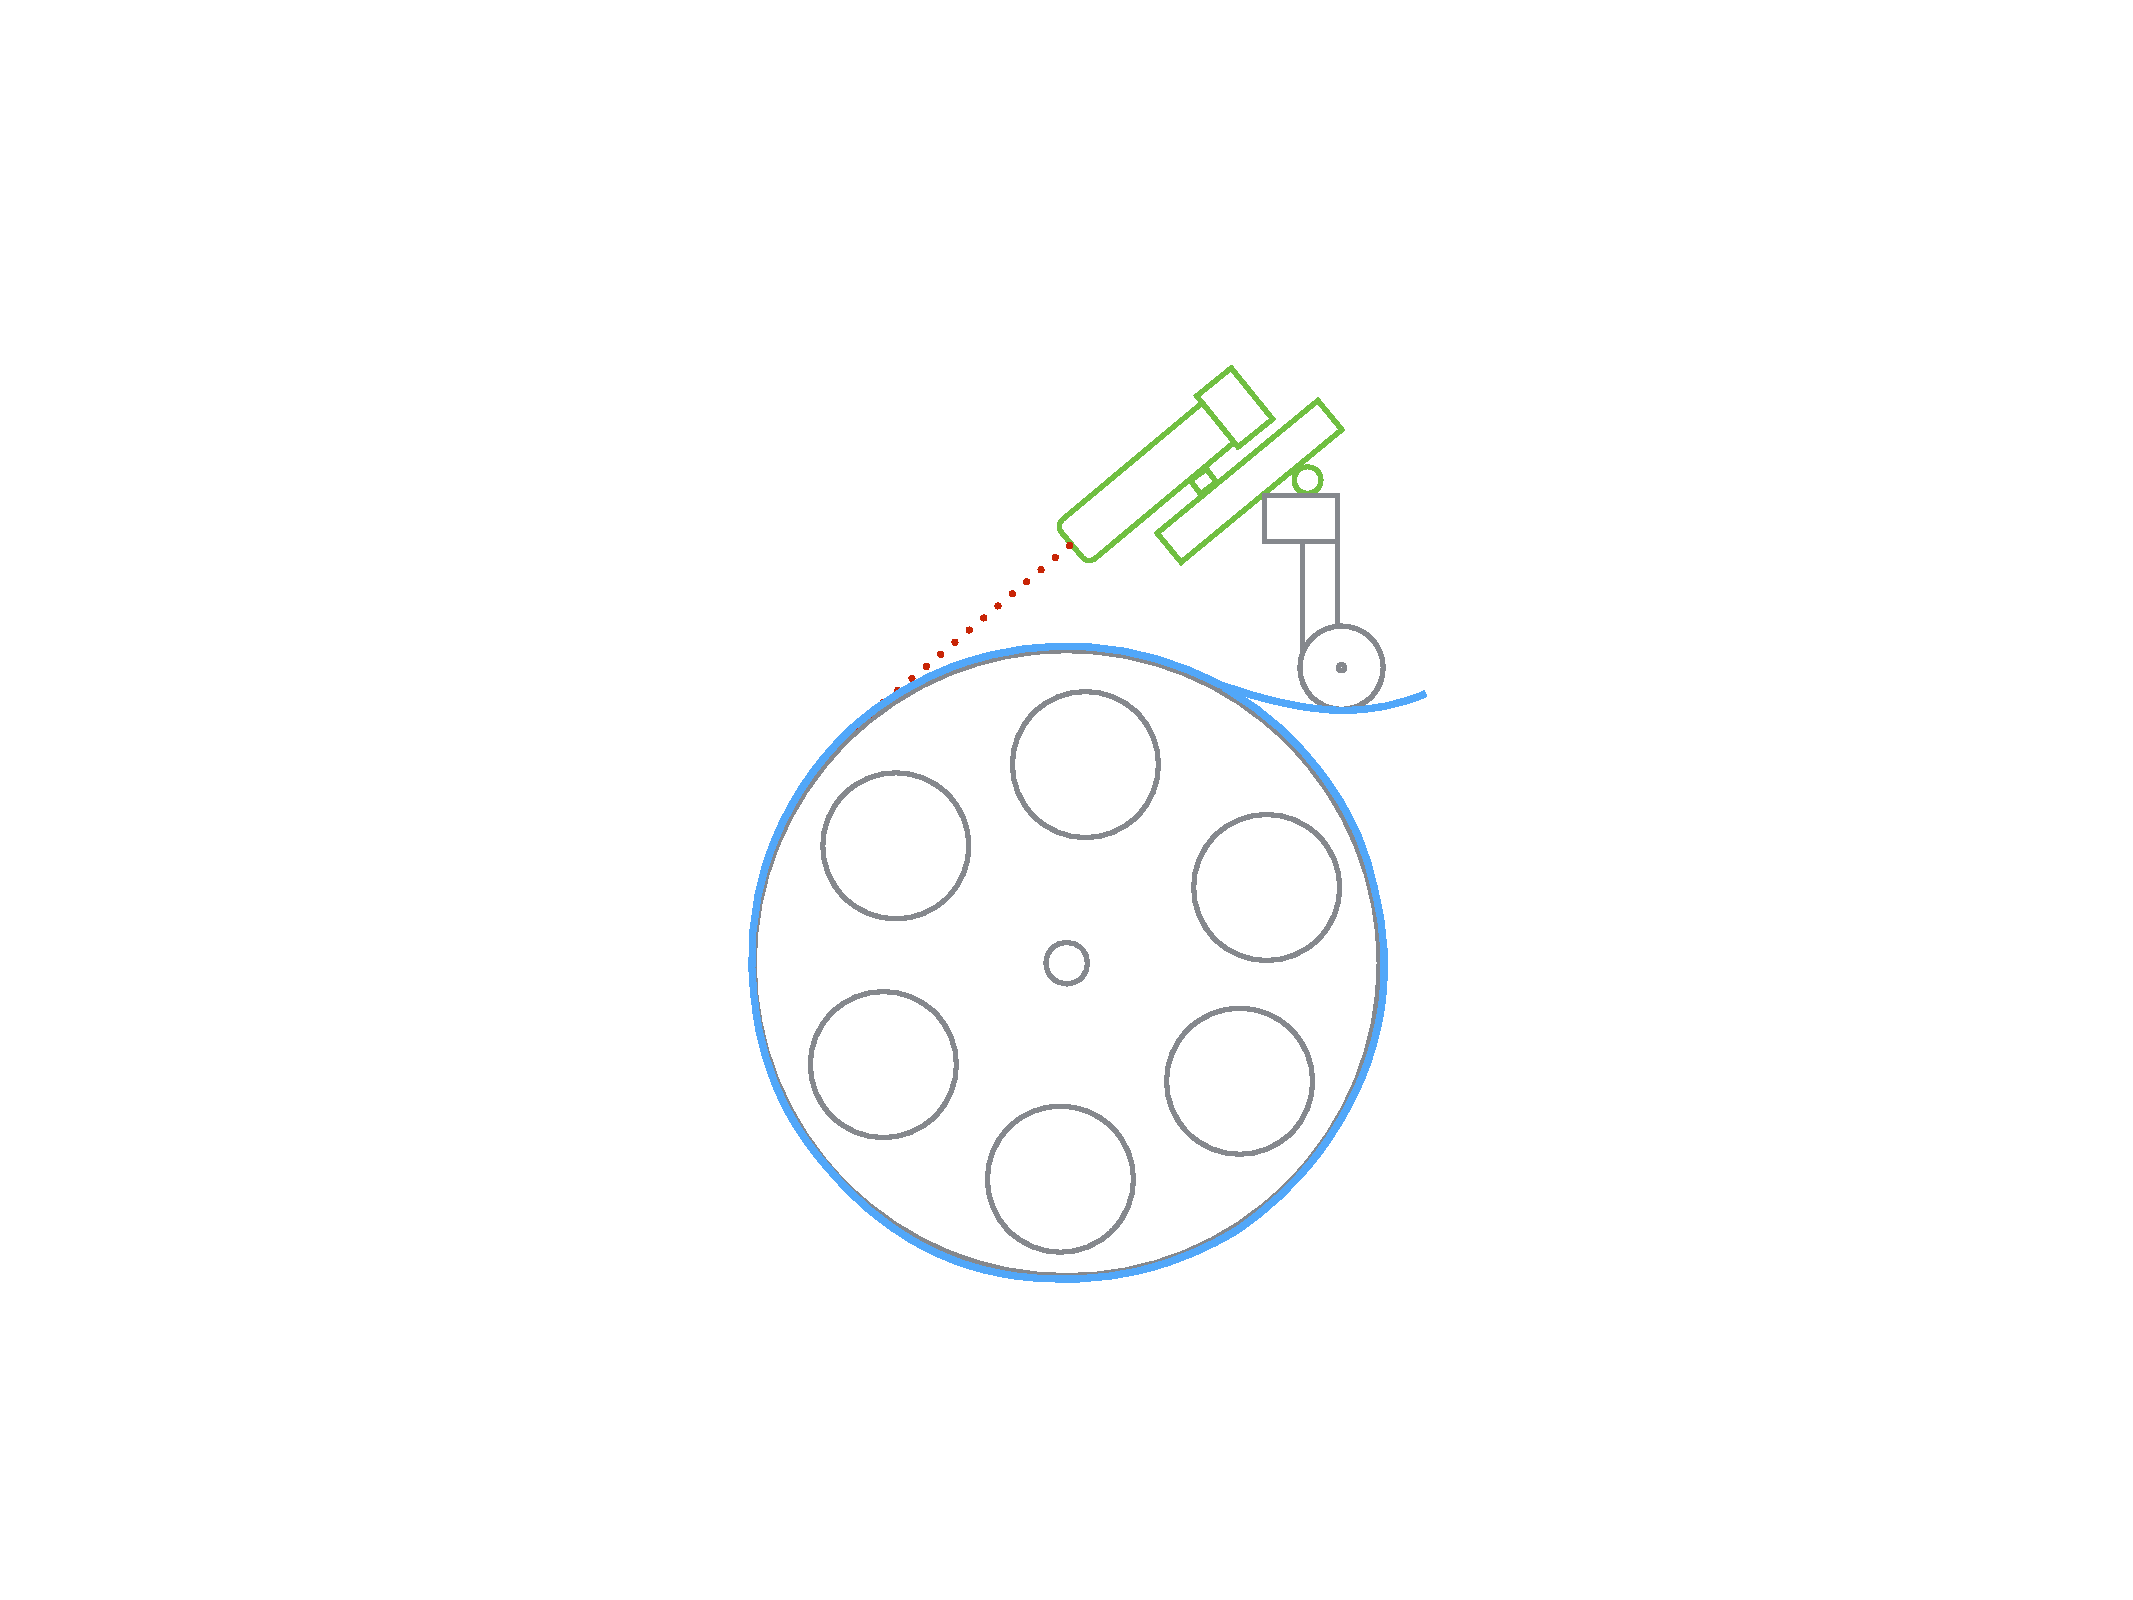
\includegraphics[width=0.5\linewidth]{figs/hardwarescheme.pdf}%
\caption{Scheme of the camera setup on the winding maschine. The camera (green) will be placed on the same slide as the positioning spool and look tangential on the wheel. \label{hardwarescheme}}
\end{center}
\end{figure}
\begin{figure}[tb]
\begin{center}
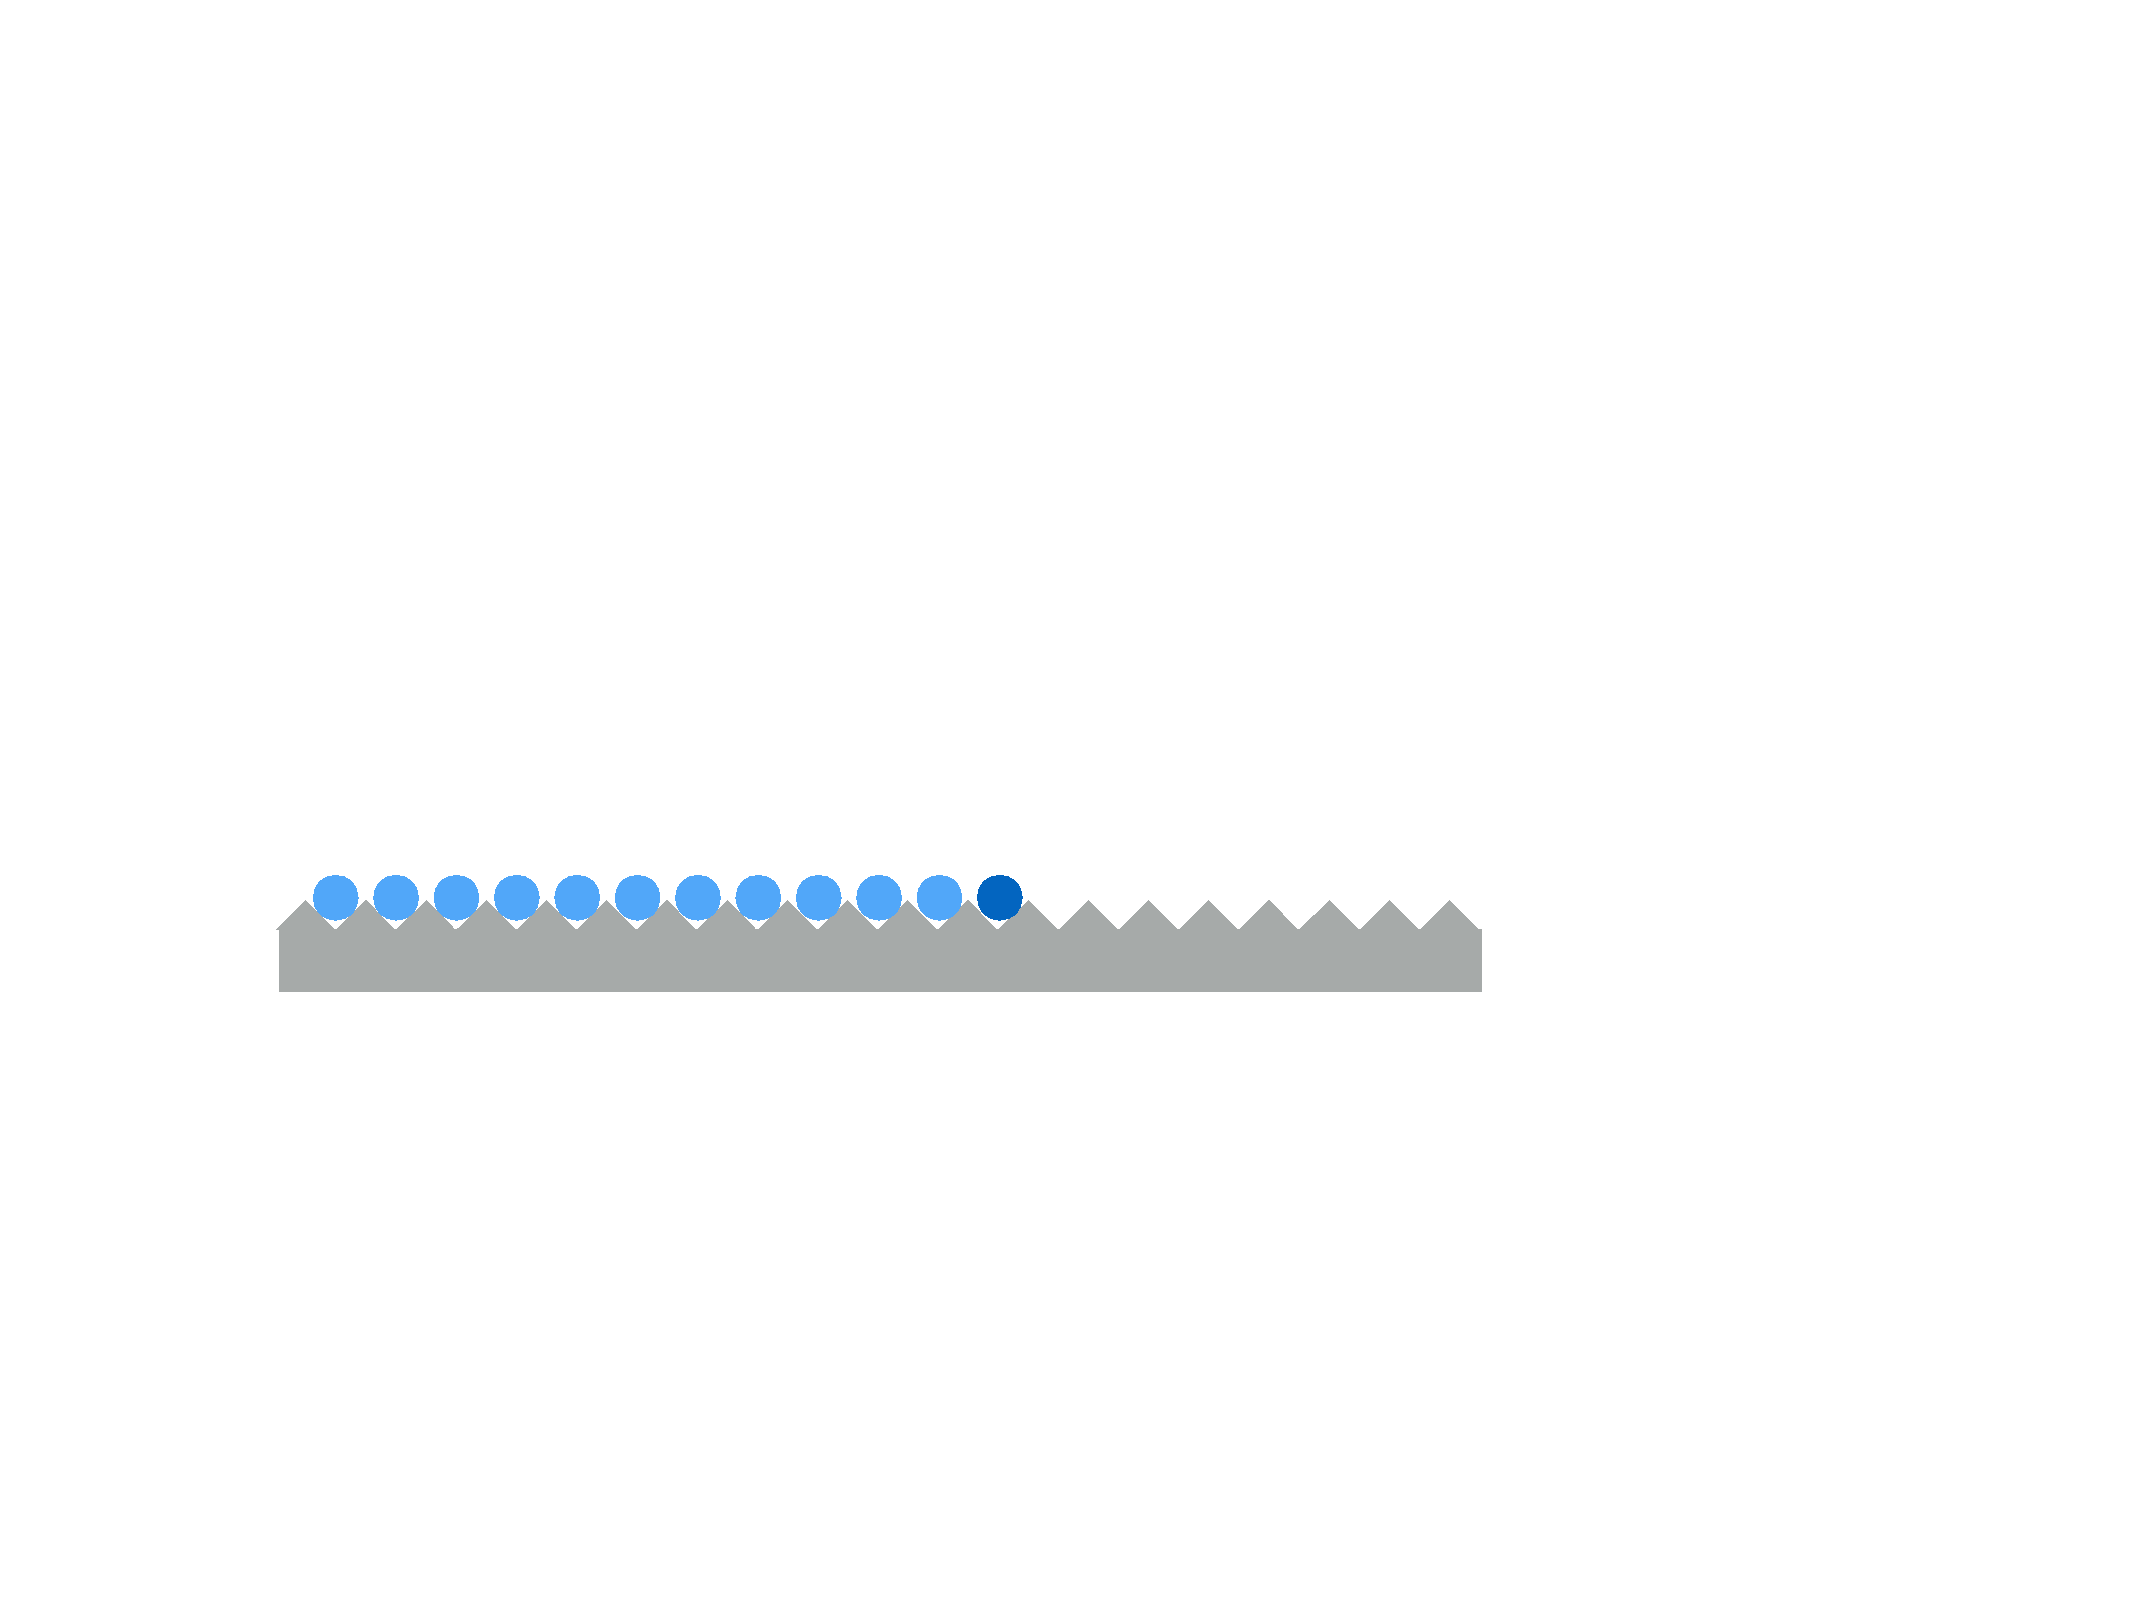
\includegraphics[width=0.5\linewidth]{figs/viewscheme.pdf}%
\caption{Scheme of the view if the camera looks tangential on the wheel. Fibres in the first layer are guided by the threat in the wheel. The current fibre is marked in dark blue.\label{viewscheme}}
\end{center}
\end{figure}

Despite of the many influences which have a bearing on the fibre positioning, there are only two different effects which can be observed during the winding process. On the one hand a fibre can jump in the wrong threat an leave an empty space (see Fig. \ref{fig:errors1})).On the other hand a fibre is able to lie down in the next layer (see Fig. \ref{fig:errors2}).
\begin{figure}[ht]
\centering
\subfigure[]{
   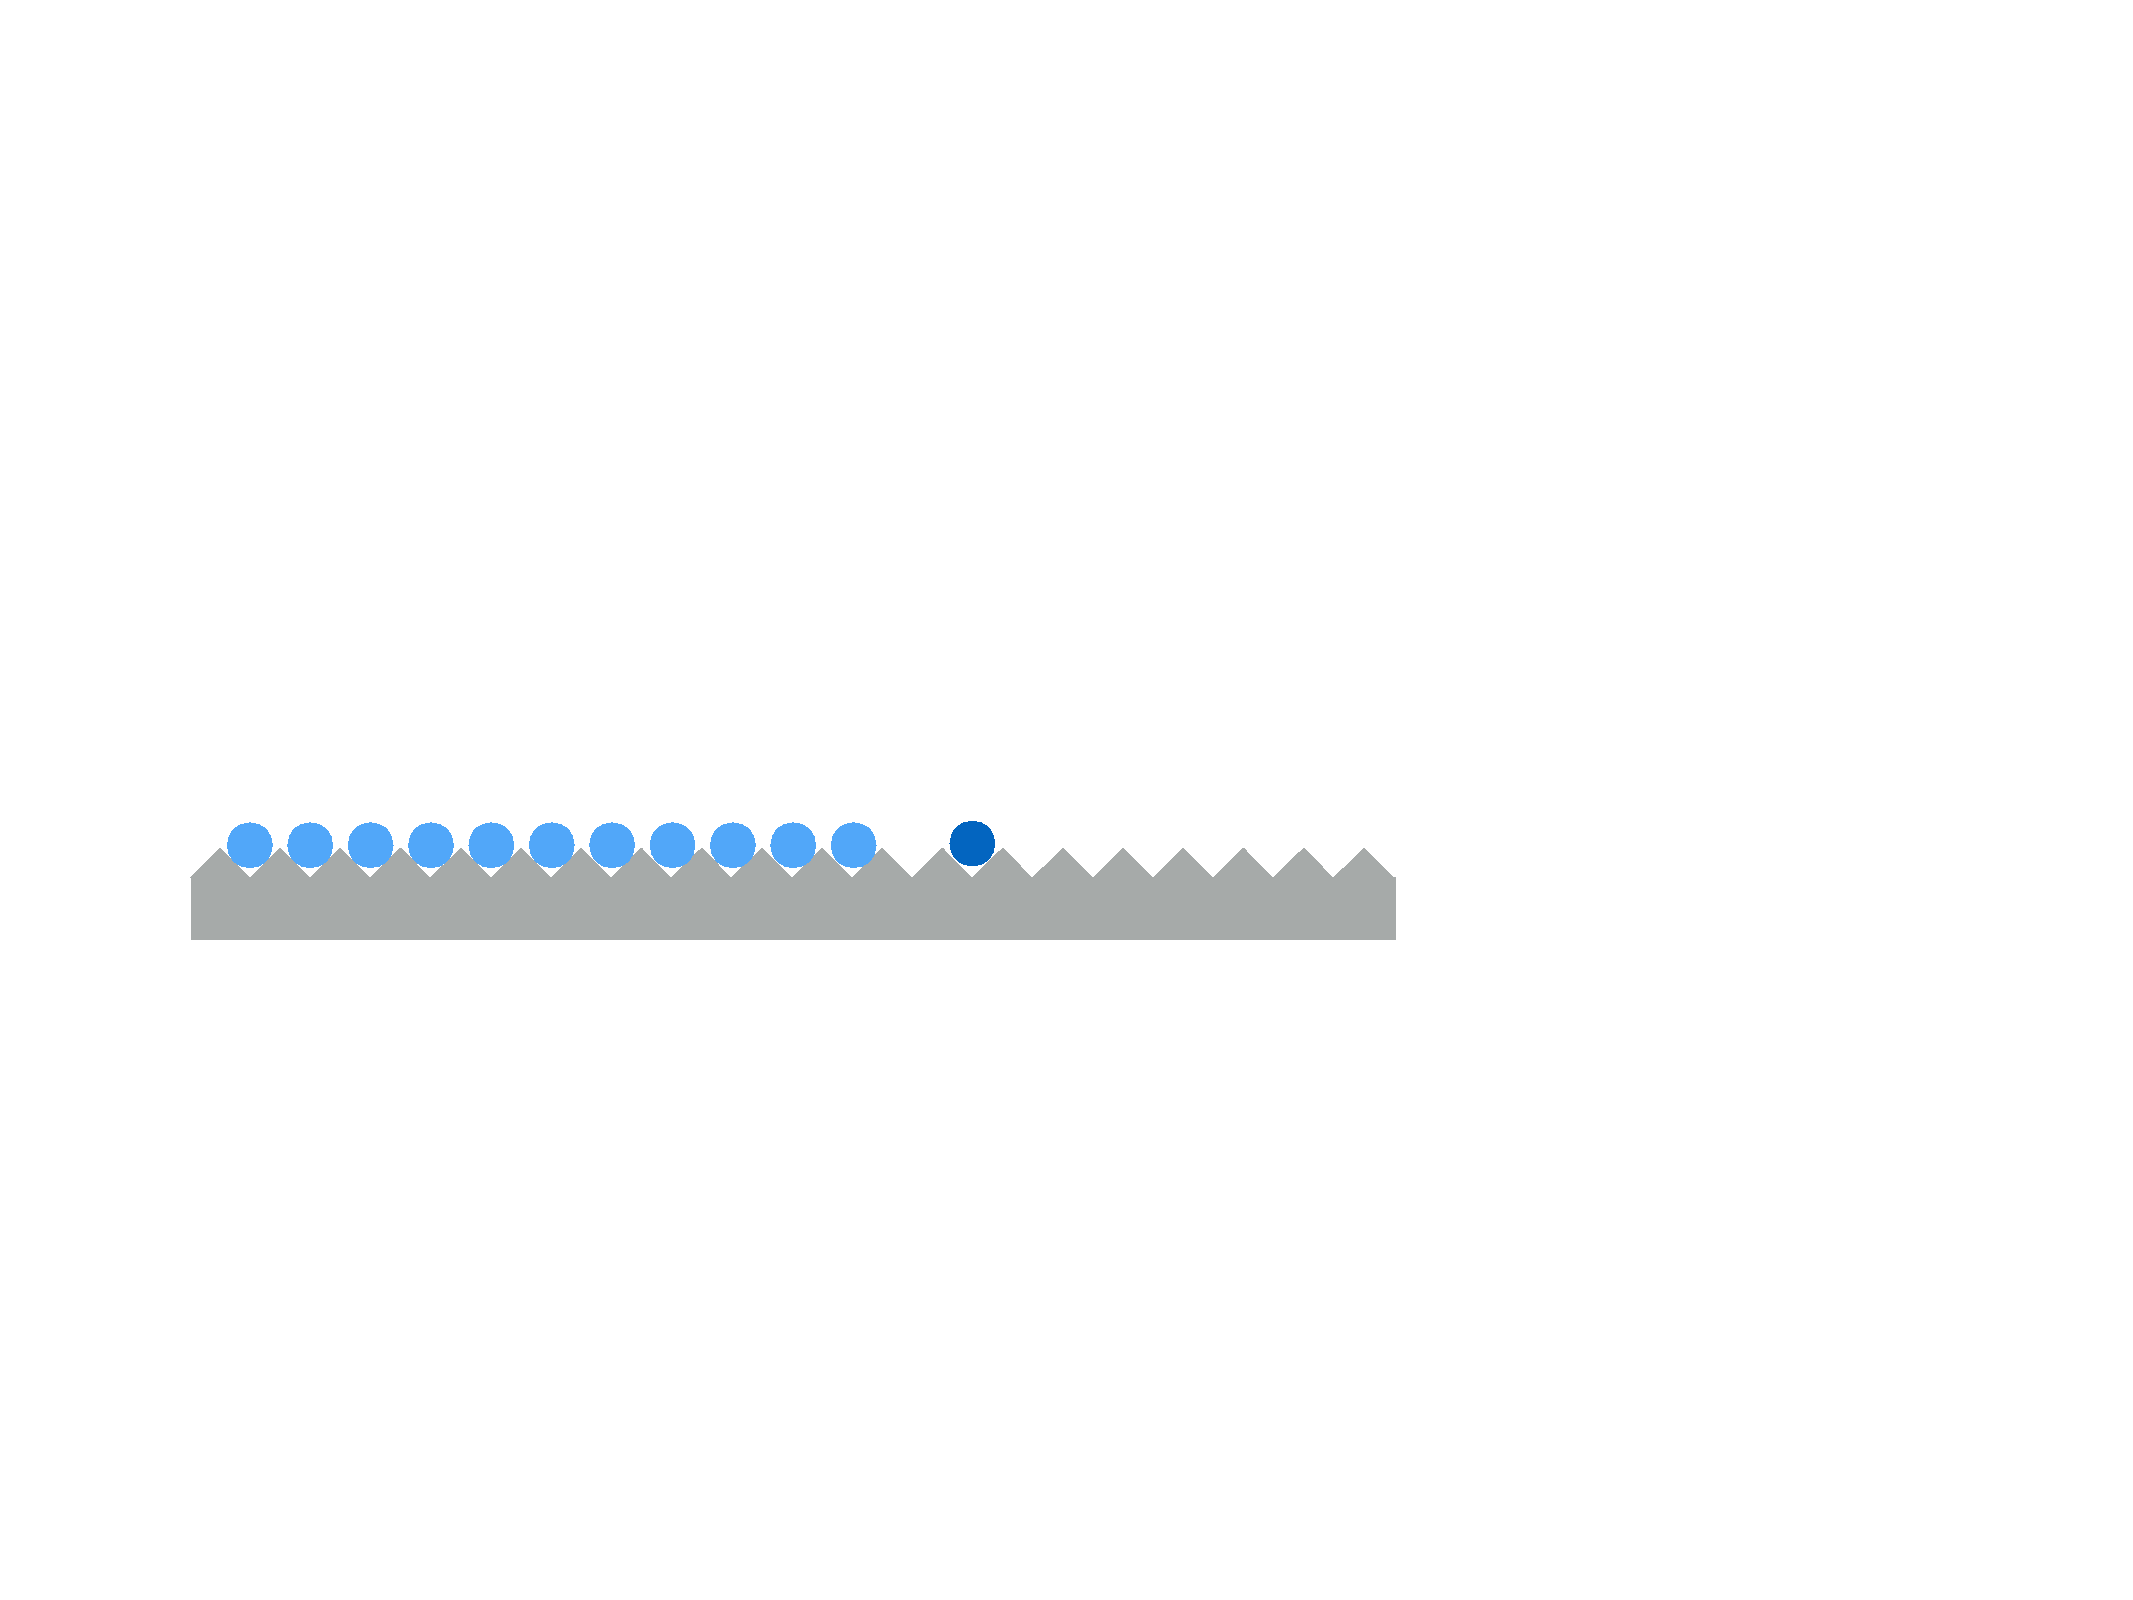
\includegraphics[width=0.4\textwidth] {figs/viewempty.pdf}
   \label{fig:errors1}
 }
\quad
 \subfigure[]{
   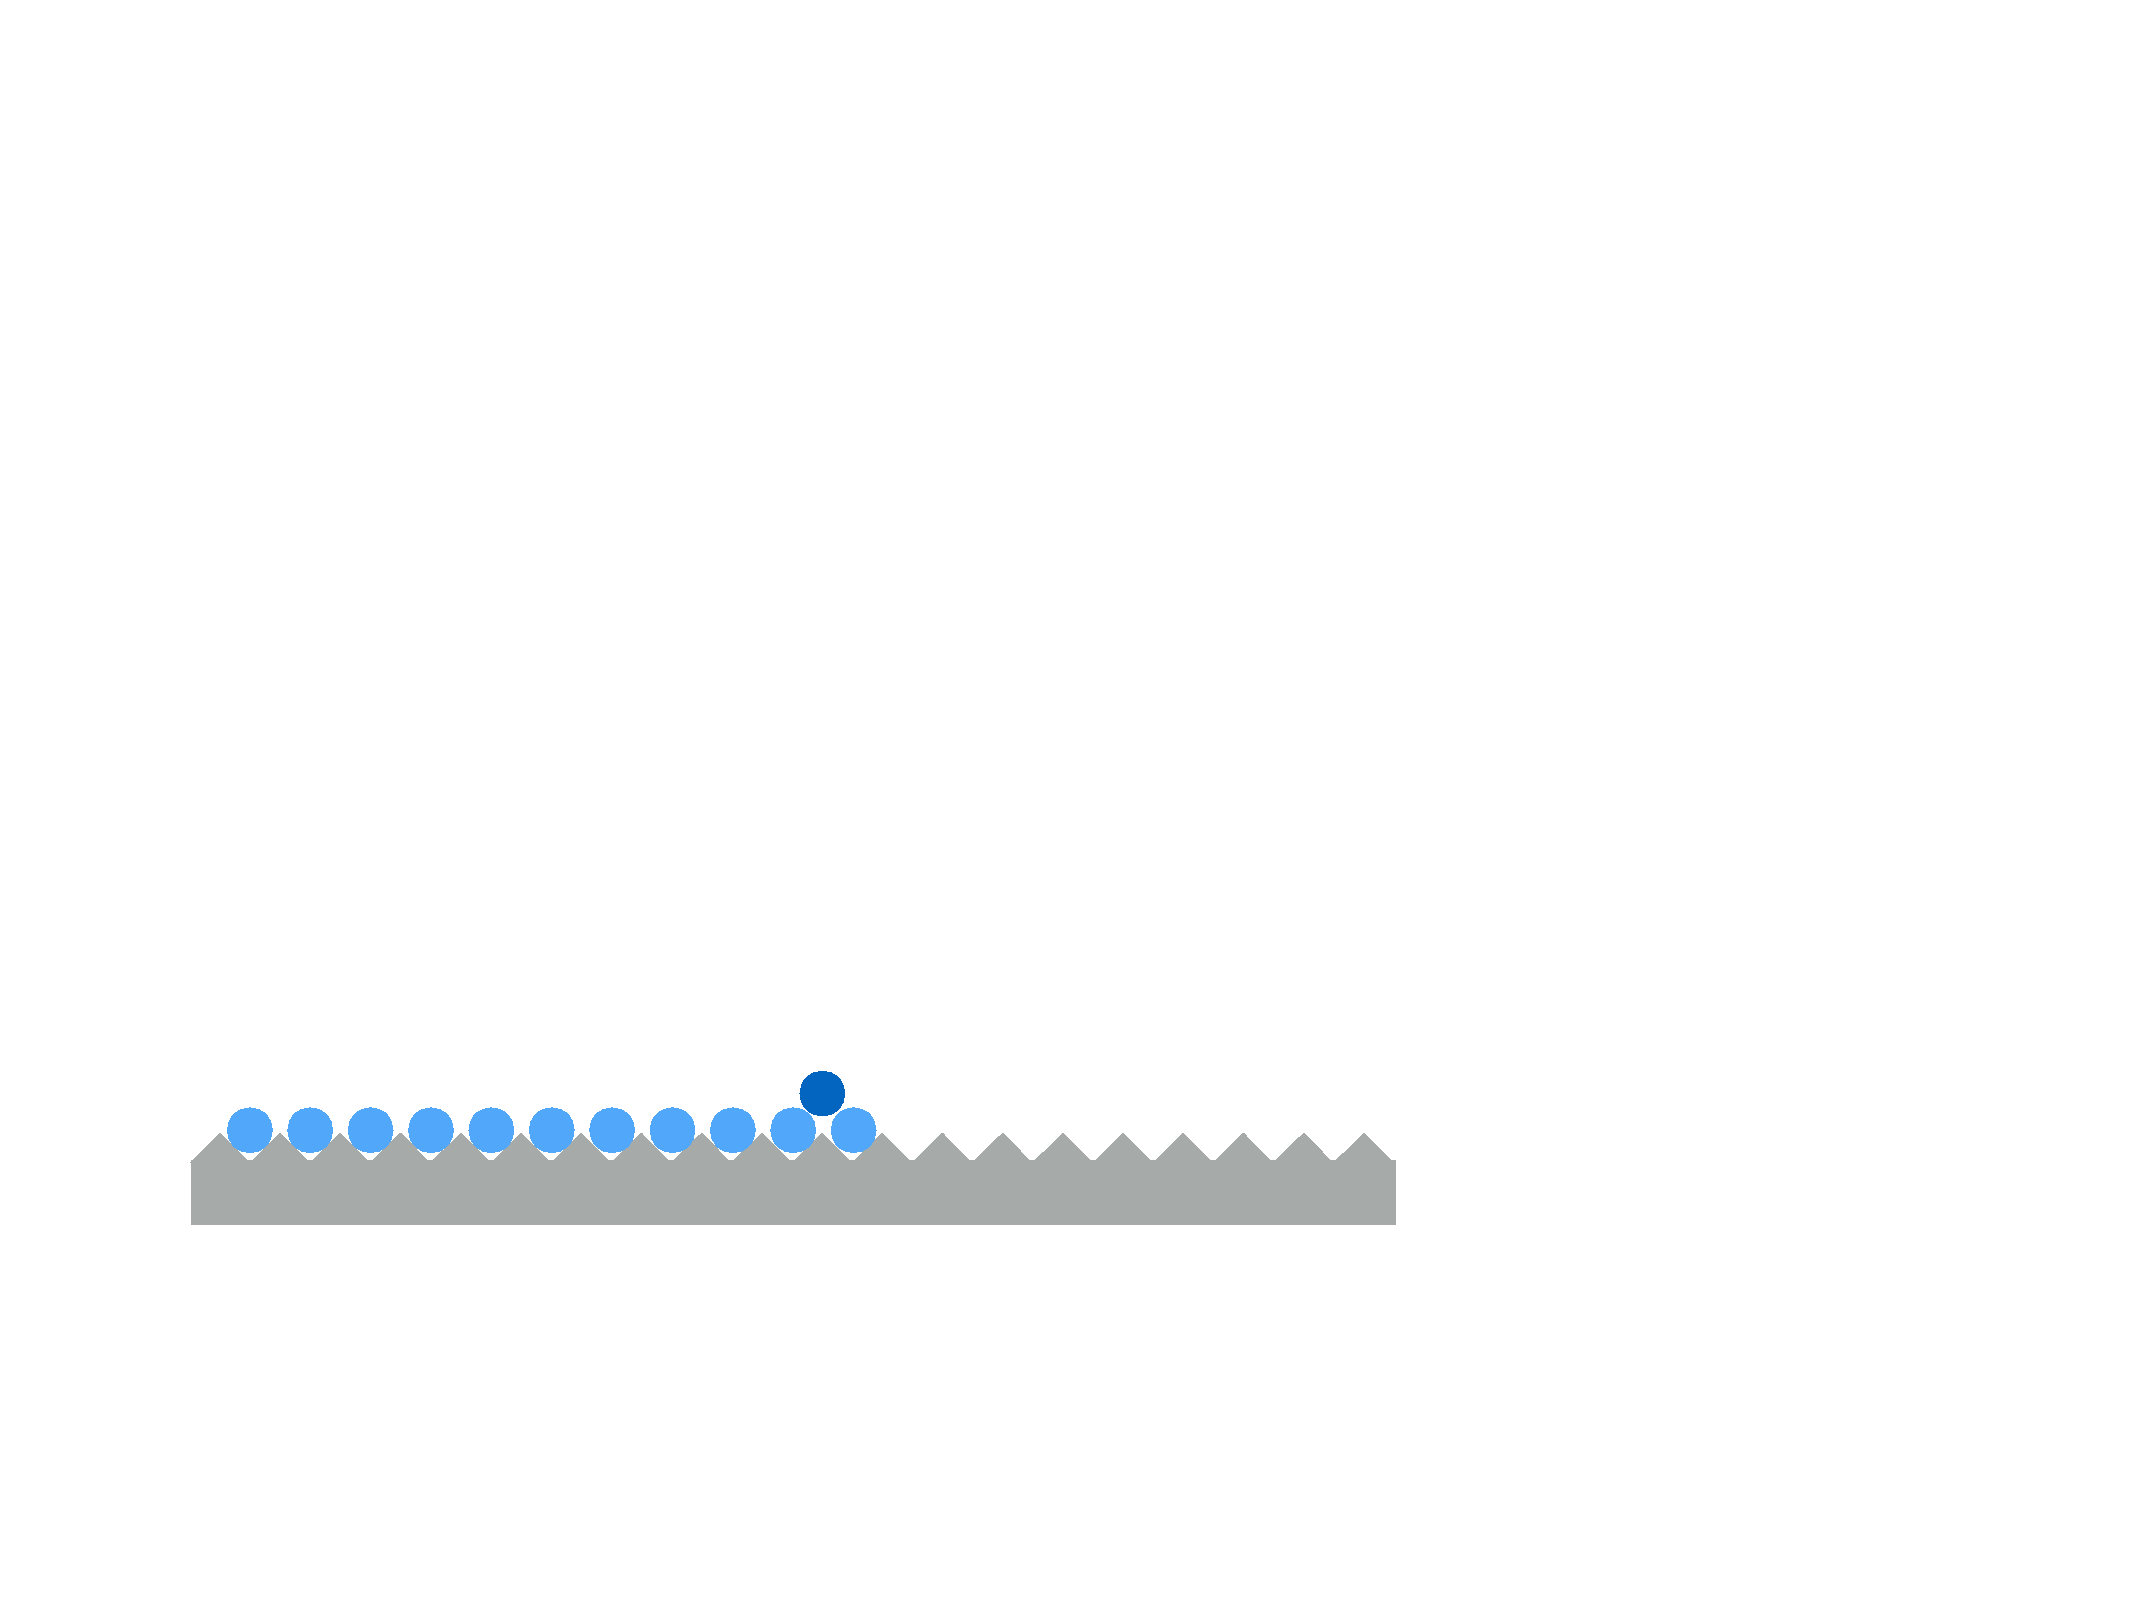
\includegraphics[width=0.4\textwidth] {figs/viewjump.pdf}
   \label{fig:errors2}
 }
\label{errors}
\caption{Two different defects which can occur during the winding process. In (a) the current fibre jumped in the wrong threat and leave an empty space. (b) shows a fibre lying in the wrong layer.}
\end{figure}

A picture of the current hardware setup is shown in Fig. \ref{CameraOnMaschine}. The camera can be adjusted by a ball head. Unfortunately the lens has no possibilty to adjust the focus, so that another slide is used for this.
\begin{figure}[tb]
\begin{center}
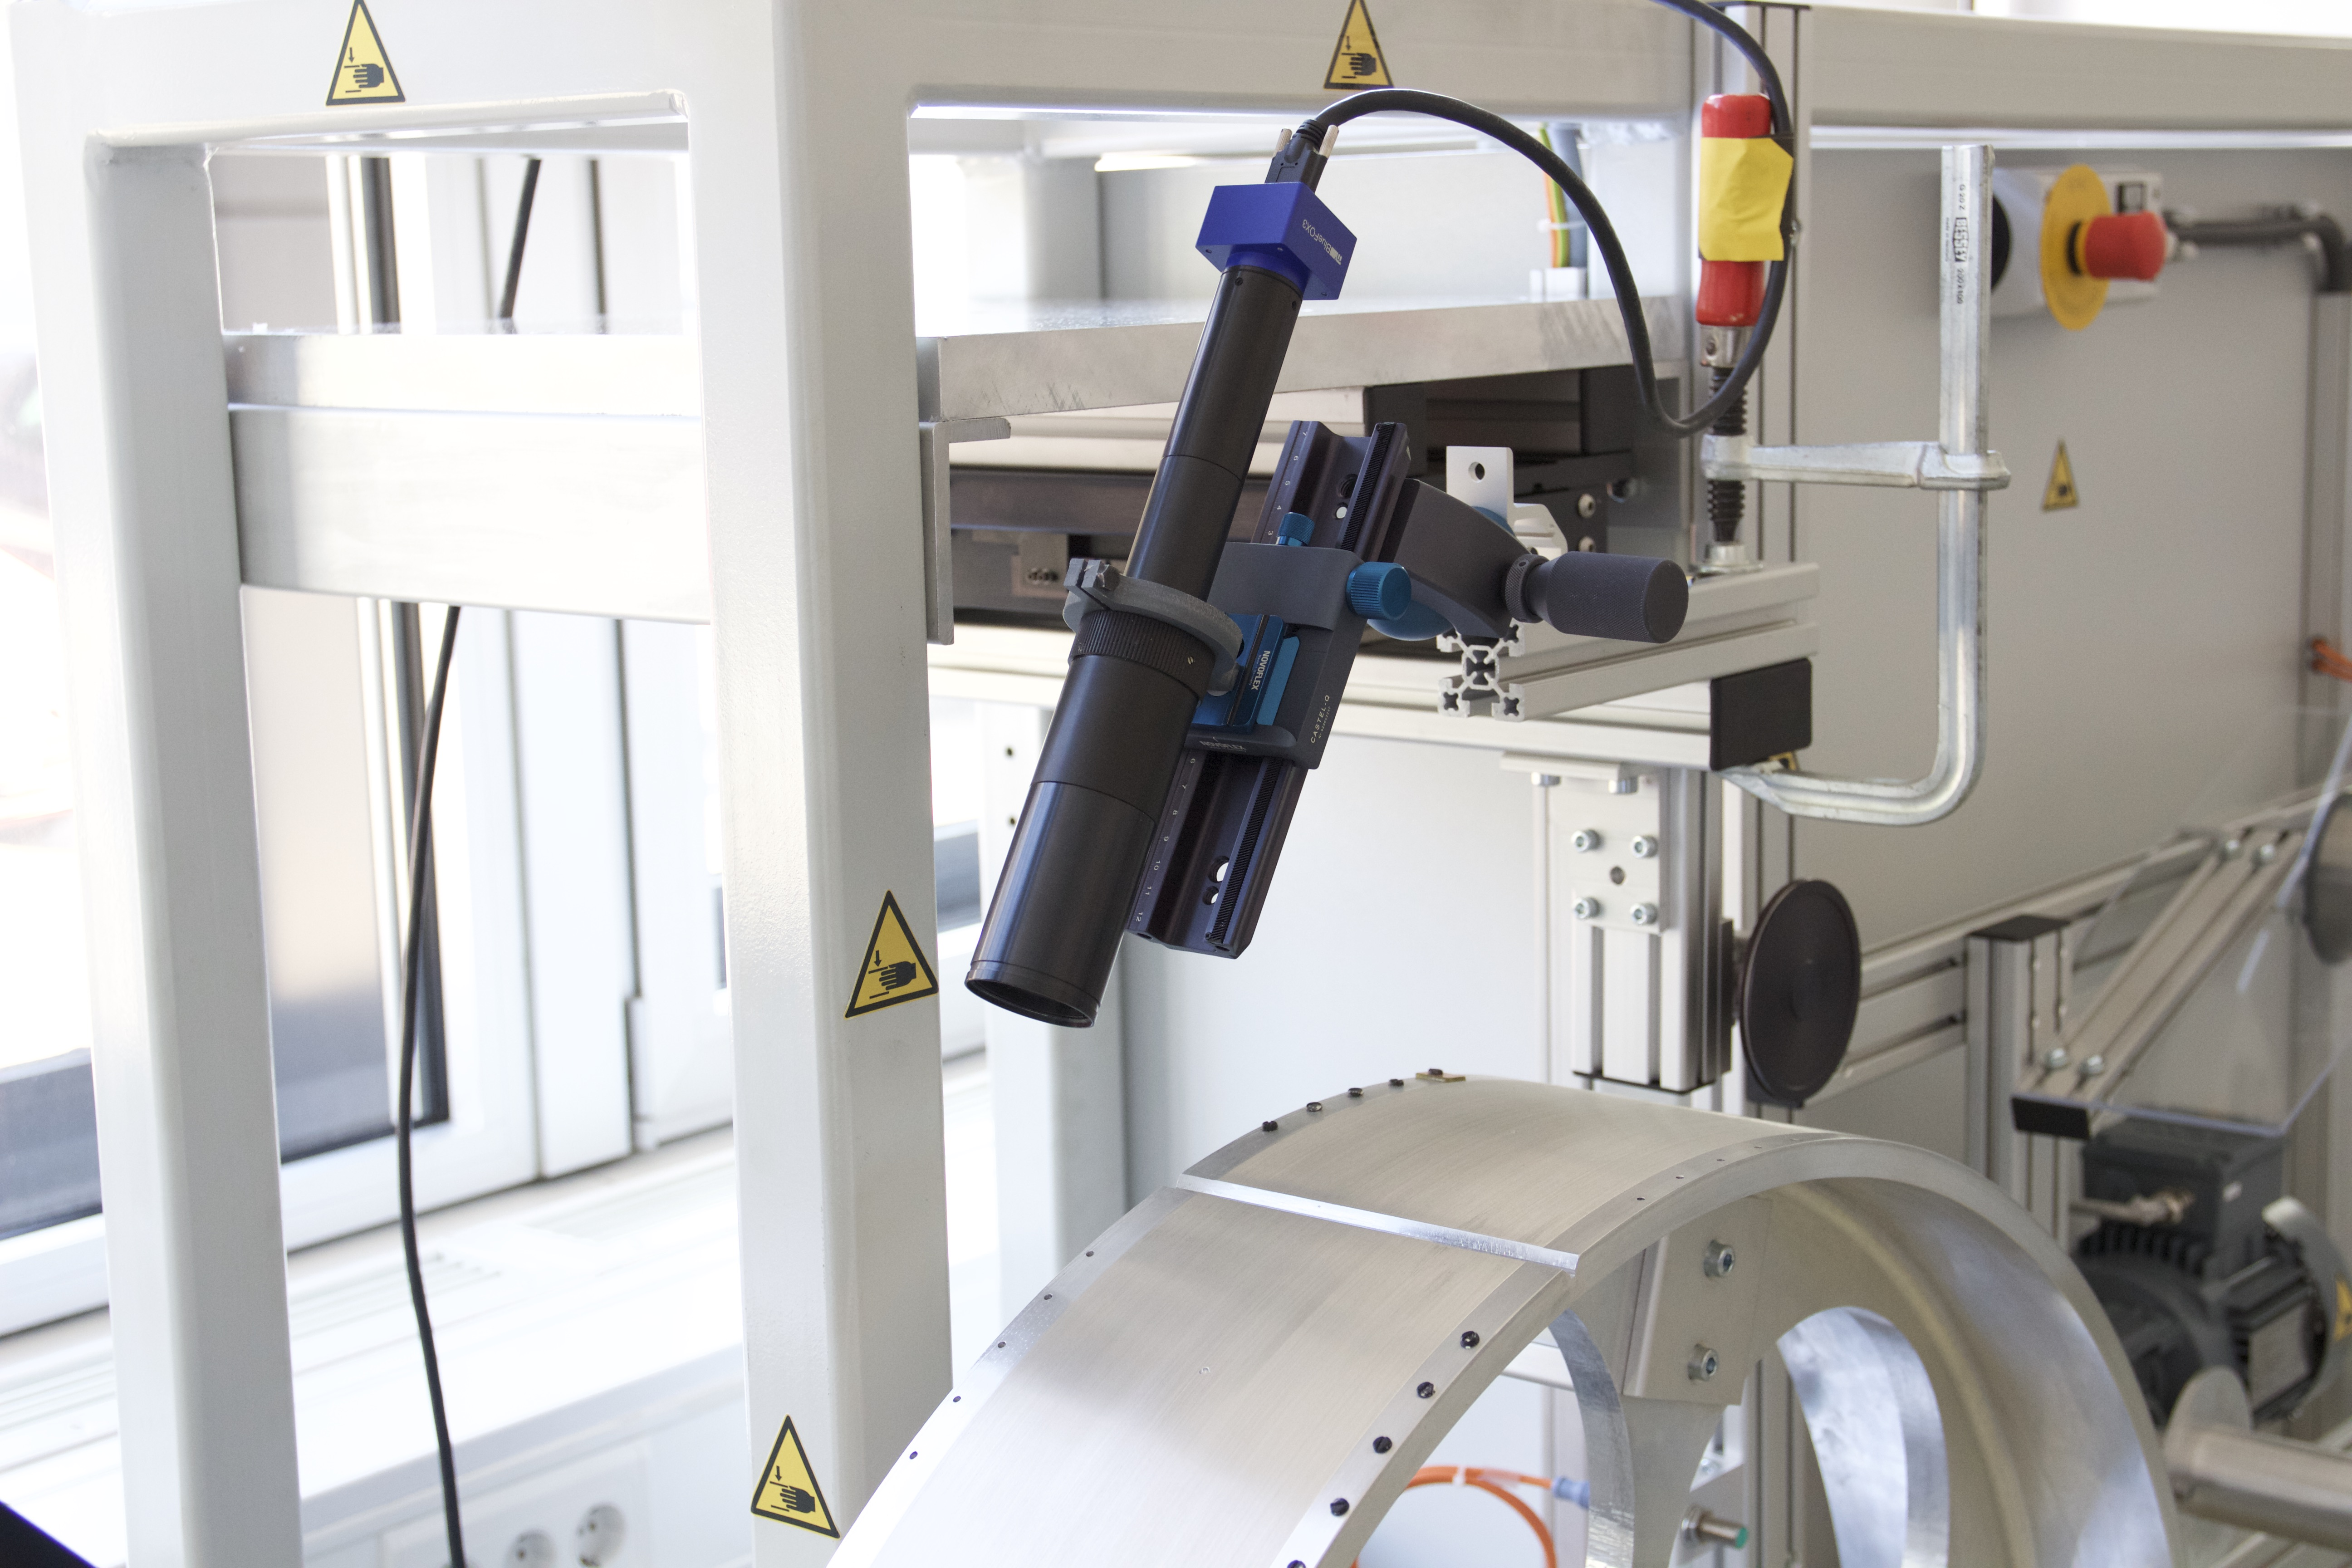
\includegraphics[width=0.5\linewidth]{figs/camera.jpeg}%
\caption{Camera setup mounted on the winding machine.\label{CameraOnMaschine}}
\end{center}
\end{figure}

\section{Software}
\label{sec:Software}

The picture of the camera is supposed to be controlled with a pattern recognition software. This insures, that no person has to be present the whole winding time and have a look on the camera picture. 

For this reason a pattern recognition software based on the open source library \emph{OpenCV}. 

\section{Results}
\label{sec:Results}

Show results of the working software.

\section{Summary}
\label{sec:Summary}

Short summary




\addcontentsline{toc}{section}{References}
\setboolean{inbibliography}{true}
\bibliographystyle{LHCb}
\bibliography{main,LHCb-PAPER,LHCb-CONF,LHCb-DP,LHCb-TDR,scifi}

\end{document}
